\chapter{基于混合模型与边界增强的极化SAR目标分类}
\section{引言}
% 问题引入
深度卷积神经网络(DCNN)由于其对大规模数据进行端到端的学习能力以及强大的特征学习能力,在极化SAR图像分类领域取得了显著的成果\citing{9625939,8771134,liu2019task}。DCNN的优越分类性能依赖于数量充足的高质量标记样本,而极化SAR样本标注工作都是通过人工标记完成,很可能因为人工标注错误、自动标注辅助技术误差、地面覆盖类型不准确等因素存在错误标记的情况,引入标签噪声\citing{tu2020robust,ni2022dnn}。DCNN方法在存在标签噪声的训练集中训练时,由于其强大的拟合能力甚至会学习到噪声的特征,出现过拟合的现象,导致分类性能有限\citing{malach2017decoupling,bengio2009curriculum}。而现有的大多数基于DCNN的极化SAR图像分类方法都是在理想的训练集中完成模型训练,很少有考虑标签噪声问题。因此研究对标签噪声的极化SAR图像分类方法具有重要的价值与意义。

% 本章方法
本章着力于含标签噪声的极化SAR图像分类方法研究,提出了一种基于混合模型估计与边界增强的极化SAR图像分类方法。首先,根据噪声样本与干净样本的损失函数分布差异特性,使用混合模型对分布差异进行拟合,以估计样本的噪声概率。其次,根据极化SAR图像标签噪声更多存在于类别边界区域特性,通过捕获类别边界区域,对边界样本施加额外的惩罚,充分利用边界样本信息。最后,基于改进的自学习优化损失函数,训练过程中通过引入模型的预测来增加感知项,对损失函数进行纠正,完成模型的鲁棒参数优化过程。

\section{有限混合模型}
DCNN模型在含标签噪声样本集上训练时,总是先学习简单的分类规则,之后再花足够的时间来对错误信息进行过拟合\citing{arazo2019unsupervised}。相比于干净的标记样本,随机标记的错误样本需要更长的时间来学习,这意味着有噪声样本在训练的前期阶段具有更高的损失,这使得干净样本与噪声样本可以通过损失值的分布情况进行区分。由于对观测值的建模能力,有限混合模型适用于估计干净样本与噪声样本的损失分布估计的场景。

有限混合模型(Finite Mixture Model, FMM)是一种用于描述观测数据生成过程的概率模型\citing{mclachlan2019finite}。该模型假设观测的数据是由有限个概率分布组合而成的混合分布,而每个成分分布对应一个潜在的类别,混合模型需要考虑这些类别之间的不同权重。

在有限混合模型中,假设观测数据来自于K个不同的成分,每个成分对应一个概率分布。对于一维数据而言,有限混合模型的概率密度函数可以表示为:
\begin{equation}
  f(x)=\sum_{k=1}^{K}\pi_k \cdot f_k(x)
\end{equation}

其中,$f_k(x)$表示第$k$个成分分布的概率密度函数,$\pi_k$表示对应成分的权重,并且满足$\sum_{k=1}^{K}=1$。表示该数据的分布是由多个成分分布的加权和。

% 在参数估计过程中,通常使用期望最大化算法(Expectation-Maximization, EM)来估计混合模型的参数,包括成分分布的参数和权重。有限混合模型在聚类、密度估计等领域都有广泛的应用,尤其在处理多个子群体或模态的数据集时表现出色。
\subsection{高斯混合模型}
高斯混合模型(Gaussian Mixture Model, GMM)是一种将一个复杂的概率分布建模为多个高斯分布的线性组合的概率模型\citing{mclachlan2014number}。相比于单一的高斯概率密度函数,GMM能够更加灵活地适应多峰的数据。GMM的核心思想是将观察到的数据视为多个高斯分布组成的混合体,每个高斯分布为一个组成分量,而所有的分量的加权和形成了整个的混合模型。

对于一个服从高斯分布的连续随机变量$x$,其概率密度函数(PDF)可以表示为:
\begin{equation}
  \begin{gathered}
    p\left( x \right) =\frac{1}{\left( 2\pi \right) ^{1/2}\sigma}\exp \left[ -\frac{1}{2}\left( \frac{x-\mu}{\sigma} \right) ^2 \right] =\mathcal{N} \left( x;\mu ,\sigma ^2 \right)
    \\
    \left( -\infty <x<\infty ;\sigma >0 \right)
  \end{gathered}
\end{equation}
记作$x \sim \mathcal{N}(\mu,\sigma^2)$,其中,$\mu,\sigma^2$分别表示$x$的均值与方差。

对于由多个高斯变量随机混合形成的部分,记为高斯混合分布。服从高斯混合分布的连续随机变量$x$的概率密度函数可以表示为:
\begin{equation}
  \begin{gathered}
    \begin{aligned}
      p(x) & =\sum_{m=1}^M \frac{c_m}{(2 \pi)^{1 / 2} \sigma_m} \exp \left[-\frac{1}{2}\left(\frac{x-\mu_m}{\sigma_m}\right)^2\right] \\ & =\sum_{m=1}^M c_m \mathcal{N}\left(x ; \mu_m, \sigma_m^2\right)
    \end{aligned}
    \\
    \left(-\infty<x<\infty ; \sigma_m>0 ; c_m>0\right)
  \end{gathered}
\end{equation}
其中,$c_m$表示不同混合分类的权重并且满足$\sum_{m=1}^M c_m=1$。

在上述的高斯混合分布中,涉及到一组参数,用$\Theta = \{c_m, \mu_m, \Sigma_m\}$ 表示。其中,$c_m$表示每个分布的权重,$\mu_m$表示均值,$\Sigma_m$表示协方差矩阵。在考虑包含多个混合分类的情况下,这一组参数可以用来描述整个混合分布的特征。要获得对混合分布参数的准确描述,需要根据一组假设来确定这些参数的值,通过最佳的参数,来匹配观测到的数据,进而更加准确的反映真实数据的特征。图\ref{GMM}展示了二分量的GMM模型概率密度函数示意图:

\begin{figure}[ht!]
  \centering
  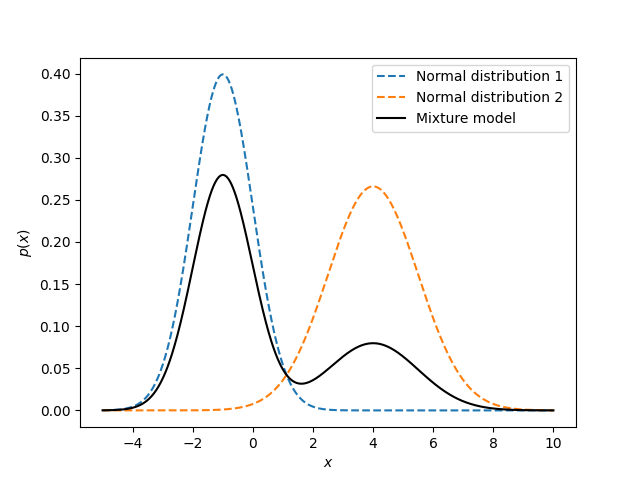
\includegraphics[width=10cm]{pic/chapter4/GMM.png}
  \caption{二分量的高斯混合模型概率密度函数示意图}
  \label{GMM}
\end{figure}

高斯混合模型具有其原理简单、对异常值不敏感等有点,已经成为当前最为普遍使用的混合模型。但是在真实场景下,数据具有非高斯性、非线性等特点,使用高斯混合模型并不能完备地描述这些数据的分布特点,例如倾斜数据、拖尾数据、有界数据等。

\subsection{贝塔混合模型}
贝塔混合模型(Beta Mixture Model, BMM)是一种概率模型,将复杂的概率分布建模为多个贝塔分布的线性组合。贝塔分布是一个定义在区间 [0, 1] 上的概率分布,通常用于描述在二项分布的贝叶斯估计中\citing{ma2011bayesian}。

对于一个服从贝塔分布的连续随机变量 $x$,其概率密度函数(PDF)可以表示为:
\begin{equation}
  \label{eq:beta1}
  p(x; \alpha, \beta) = \frac{x^{\alpha - 1} (1 - x)^{\beta - 1}}{B(\alpha, \beta)}
\end{equation}
其中,$B(\alpha, \beta)$为贝塔分布的概率密度函数,具体表示为:

\begin{equation}
  B(\alpha, \beta) = \frac{\Gamma(\alpha) \Gamma(\beta)}{\Gamma(\alpha + \beta)}
\end{equation}
其中,$\alpha$ 和 $\beta$ 是贝塔分布的参数,$\Gamma$ 表示伽玛函数。对于由多个贝塔分布随机混合形成的部分,记为贝塔混合分布。服从贝塔混合分布的连续随机变量 $x$ 的概率密度函数可以表示为:
\begin{equation}
  \label{eq:beta}
  \begin{gathered}
    \begin{aligned}
      p(x) & = \sum_{m=1}^M c_m \frac{x^{\alpha_m - 1} (1 - x)^{\beta_m - 1}}{B(\alpha_m, \beta_m)} \\
           & = \sum_{m=1}^M c_m \text{Beta}(x; \alpha_m, \beta_m)
    \end{aligned}
    \\
    (0 < x < 1; c_m > 0; \sum_{m=1}^M c_m = 1; \alpha_m, \beta_m > 0)
  \end{gathered}
\end{equation}
其中,$c_m$ 表示不同混合分类的权重,满足 $\sum_{m=1}^M c_m=1$。

在贝塔混合分布中,参数集为 $\Theta = \{c_m, \alpha_m, \beta_m\}$。其中,$c_m$ 表示每个贝塔分布的权重,$\alpha_m$ 和 $\beta_m$ 分别表示每个贝塔分布的形状参数。为了描述整个混合分布的特征,需要通过一组假设,从观测到的数据中确定这些参数的值。这一过程旨在使混合分布的参数最佳匹配观测到的数据,以更准确地反映实际数据的特征。图\ref{BMM}展示了二分量的BMM模型概率密度函数示意图:
\begin{figure}[ht!]
  \centering
  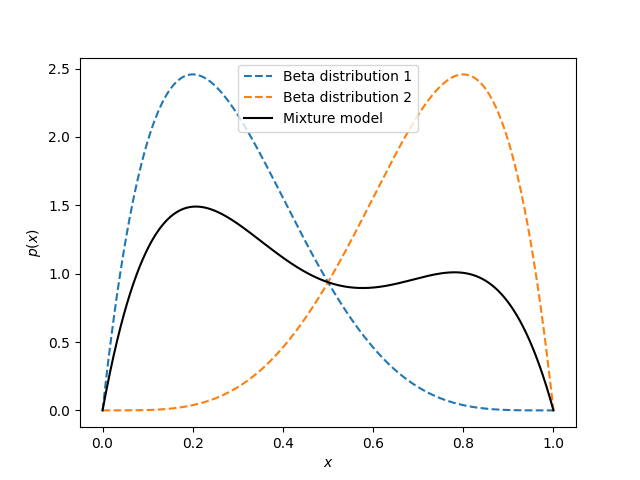
\includegraphics[width=10cm]{pic/chapter4/BMM.png}
  \caption{二分量的贝塔混合模型概率密度函数示意图}
  \label{BMM}
\end{figure}

\section{混合模型与边界增强的标签噪声分类方法}
\subsection{标签噪声问题建模}
% 由于极化SAR的复杂成像机制,获取足够数量的训练样本是一项非常耗时和耗力的任务。而且,现有数据集中的标注虽然可能近似完美,但实际上存在一些错误标记的样本。这种标签噪声可能由于人工标记的错误、边界区域的模糊性以及场景图像的错误等原因产生。在使用混合标签噪声的训练集进行训练时,模型可能学习到噪声样本的特征,从而对原有的分类规则造成干扰,导致过拟合的问题。
给定一个包含N个类别的干净PolSAR数据的训练集,表示为:
\begin{equation}
  (X, Y^{(c)})=\{(x_1,y_1^{(c)}),\ldots,(x_N,y_N^{(c)})\}
\end{equation}
该数据来源于分布$D=X \times Y$。假设存在一个函数$\mathcal{F}:Y^{(c)} \rightarrow Y^{(n)}$,该函数向标签$Y^{(c)}$引入噪声,将$\mathcal{F}$应用于$(X, Y^{(c)})$得到一个带有噪声的训练数据集,表示为:
\begin{equation}
  (X, Y^{(n)})=\{(x_1,y_1^{(n)}),\ldots,(x_N,y_N^{(n)})\}
\end{equation}
其中$Y^{(n)}$是原始干净标签$Y^{(c)}$和被污染的标签$Y^{(n)} \neq Y^{(c)}$的组合。

假定标签$y_i^{(c)}$被噪声函数污染成$y_i^{(n)}$,存在对称噪声源与非对称噪声源两种类型。对称噪声源模型是将真实标签以相同的概率随机翻转到其他类别,服从均匀分布,表达式如下:
\begin{equation}
  P(y_i=y_i^{(n)} \mid y_i^{(c)})=\frac{1}{N-1}
\end{equation}

非对称噪声源模型是按照根据某种固定的规则进行标签映射操作,将真实标签以随机概率翻转到其他的某个类别。图\ref{fig:noisy_type}展示了两种类型噪声源的噪声转移矩阵示意图。
\begin{figure}[ht!]
  \subfloat[]{
    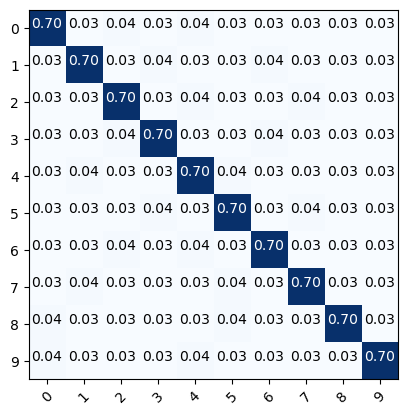
\includegraphics[width=7.04cm]{pic/chapter4/Random.png}
  }
  \subfloat[]{
    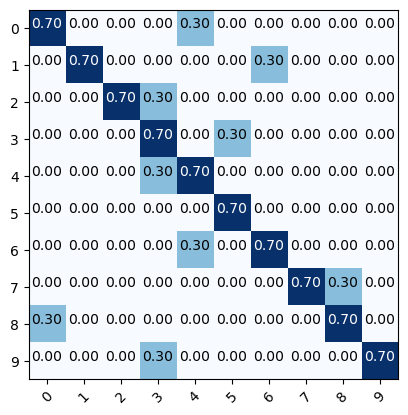
\includegraphics[width=7.04cm]{pic/chapter4/One.png}
  }
  \caption{30\%比例噪声转移矩阵示意图。(a)对称噪声 (b)非对称噪声}
  \label{fig:noisy_type}
\end{figure}

从干净分布$D$中随机选择一个测试集$(X_T, Y_T)$。目标是使用带有噪声的数据集$(X, Y^{(n)})$训练一个分类器模型$M:X \rightarrow Y$,以确保对干净测试集$(X_T, Y_T)$的鲁棒性泛化,并且在训练过程中无法访问原始的干净标签$Y_c$。

% 深度网络模型在混合噪声的数据集上训练时,总是会先学习简单的干净样本特征,之后再花更长的时间来拟合随机的标签噪声。这意味着噪声样本在训练的前期具有更高的损失,这样可以通过损失的分布来区分噪声和干净样本。

% 本章中,为了解决极化SAR图像中的标签噪声问题,提出了一个端到端的标签噪声条件下的极化SAR图像分类方法,基于贝塔混合分布引导的标签噪声下极化SAR图像分类方法。首先利用贝塔混合概率模型拟合噪声样本、干净样本的损失函数分布以区分噪声样本和干净样本。然后,设计动态损失函数,结合模型的预测类别对噪声样本进行校正。同时,通过对边界样本损失增强实现模型对边界样本的关注提升。将上一章的插件式极化信息提取方法作为本分类任务的前置模块,旨在应用深层次极化信息来辅助该特定的分类任务,并提升该任务下的分类精度。

% 近年来,各种应对于标签噪声问题的鲁棒性学习方法层出不穷,文献\cite{zhang2021understanding,wang2018iterative}指出,尽管基于深度网络模型的分类网络具有对噪声标签的记忆能力,但在训练过程中是先学习主要的分类规则,然后才开始记忆噪声的分类模式。本章对此进行了进一步的研究,提出了一个端到端的标签噪声条件下的鲁棒性训练方法。


\subsection{基于混合模型与边界增强的目标分类算法框架}

% 在极化SAR图像目标分类中,标签噪声的存在通常会导致传统分类方法性能下降,基于卷积网络的模型往往也会陷入过拟合的问题,学习到错误的分类规则。标签噪声通常是由于地物杂波、系统误差、人工标记错误等因素引入,导致训练集中包含错误的标签。为了解决这个问题,本章方法提出了一种针对极化SAR的鲁棒性分类方法。图\ref{BBM_framework}展示了BBM算法的框架图。由于深度网络模型总是趋向于先学习简单样本,之后通过足够的迭代去拟合困难的样本。在标签噪声下的深度网络训练过程中,会呈现双峰的损失函数分布情况。因此,与传统的分类方法相同,本方法首先通过深度网络进行特征提取和分类器进行分类,计算每个训练样本的损失函数。得到的损失函数值并不直接参与模型的反向传播中,而是通过二分量的贝塔混合模型来拟合所有的损失函数的分布,通过损失函数的观测值来得到贝塔混合模型的参数估计。确定噪声分量的噪声概率密度函数之后,即可根据损失函数值得到对应的样本噪声概率。其次,由于极化SAR目标分布存在空间一致性,空间连续的样本往往属于同一个类别。并且,空间连续区域标注简单,标签噪声更加趋向于出现在类别边界区域。基于该特性,还设计了边界样本增强分支,对极化SAR图像进行Pauli分解,得到对应的伪彩图,在伪彩图中利用Sobel边界提取算子并通过边界膨胀,获得图像大致的膨胀边界。对于属于膨胀边界内的样本模型应该付出更多的注意,来拟合其中的特征。最后,由于训练集数量有限,如果直接丢弃属于噪声的样本,可能会导致丢失其中必要的空间信息。因此,引入了动态的鲁棒性损失函数,即赋予模型动态的根据噪声概率去选择训练集标签或者模型预测值作为交叉熵损失的计算基准。通过以上的鲁棒性训练方法,最终获得对标签噪声具备鲁棒性的分类模型。

在极化SAR图像目标分类中,标签噪声的存在通常会导致传统分类方法性能下降,基于卷积网络的模型往往也会陷入过拟合的问题,学习到错误的分类规则。针对标签噪声问题,本章提出了基于混合模型估计与边界增强的极化SAR图像分类方法,其算法框架如图\ref{BBM_framework}所示。区别于传统的交叉熵损失优化方法,本章方法基于混合模型理论对样本损失函数进行参数估计,以区分噪声样本与干净样本。为了降低边界标签噪声样本对模型训练的影响,增强对边界样本的有效信息利用,通过Sobel算子对极化SAR图像的Pauli伪彩图进行边界提取并膨胀,对属于膨胀边界内的样本施加额外的惩罚,增强样本损失。最后,基于改进的自学习优化损失函数,结合模型预测感知项,对噪声标签进行校正,实现模型的鲁棒性训练。

\begin{figure}[h]
  \centering
  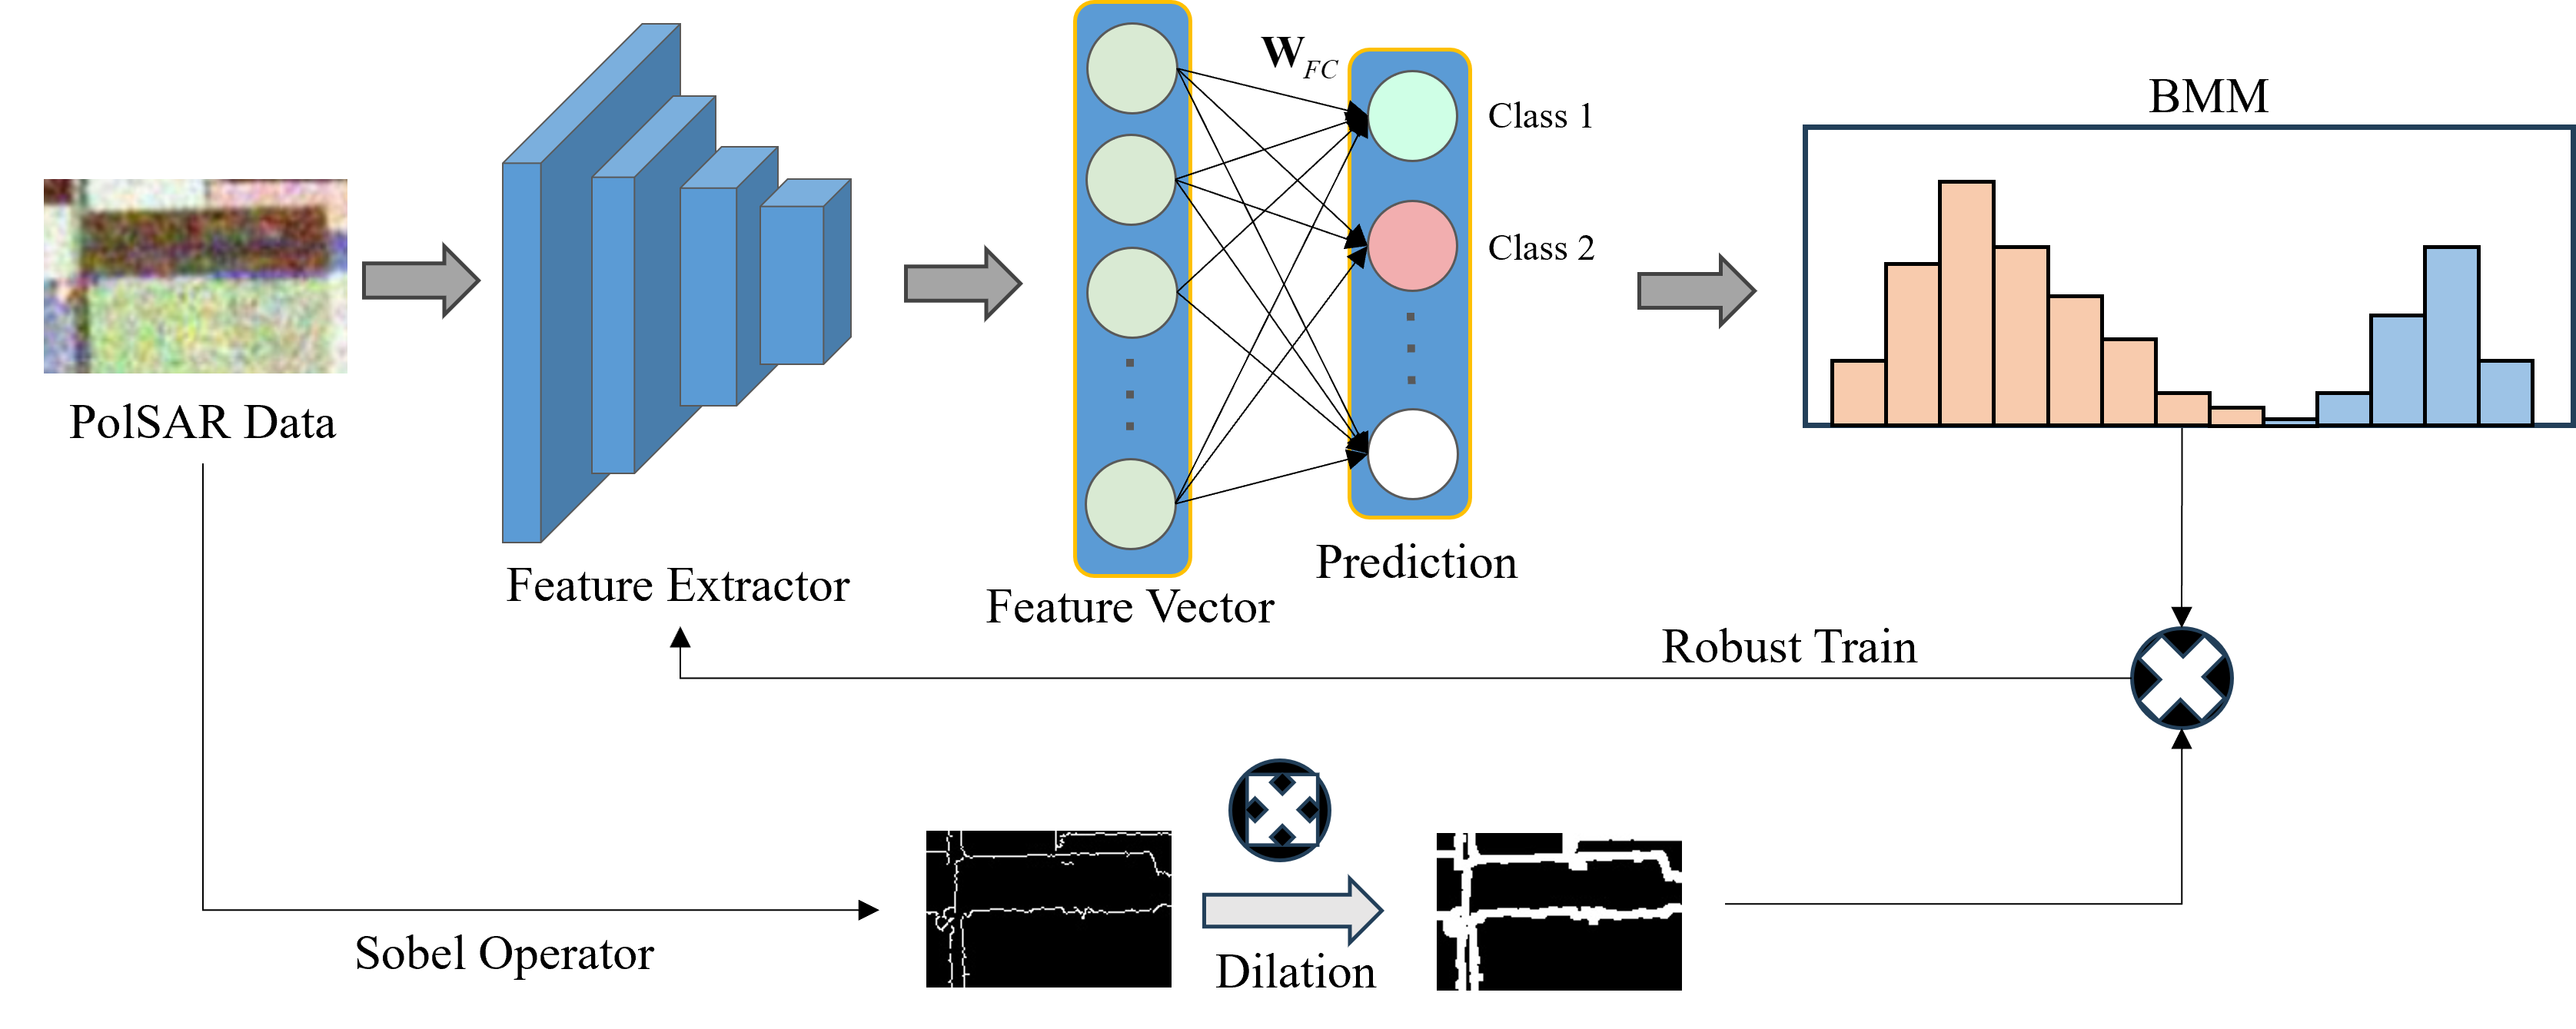
\includegraphics[width=14cm]{pic/chapter4/framework.png}
  \caption{标签噪声下鲁棒性分类算法框架图}
  \label{BBM_framework}
\end{figure}

结合上述算法框架,本章基于混合模型估计与边界增强的极化SAR图像分类方法可以表示为以下步骤:

(1)极化特征输入。极化特征具有多种表示形式,选择合适的极化特征对于分类任务具有重要意义。本章研究属于极化SAR图像分类问题,将第三章提出的双通道注意力极化信息提取方法作为本算法的前置模块,用于极化特征表示,并输入到后续网络。

(2)鉴别特征提取与分类。利用卷积神经网络,对输入的极化特征进行特征提取。通过多个堆叠的卷积、池化与激活操作,主干网络学习到极化特征的高级表征。随后,利用全连接层与激活函数,将主干网络的输出映射到不同的类别,得到对样本的预测类别。

(3)噪声概率估计。计算每个样本预测类别与标签的交叉熵损失,并基于贝塔混合模型拟合样本损失分布。利用损失值来更新迭代混合模型参数,基于更新后的模型参数计算样本噪声概率。

(4)边界样本增强。利用Sobel算子对极化SAR图像的Pauli伪彩图进行边界提取并膨胀,对膨胀边界内部的训练样本进行损失函数加权增强,以提高模型对边界信息的学习能力。

(5)自学习损失函数优化。基于自学习损失函数,利用估计的样本噪声概率,动态调整模型预测与标签真值的权重。利用改进的自学习损失函数计算损失值后,通过反向传播更新模型参数,实现模型的训练优化。

\subsection{噪声概率估计模型}
在混合标签噪声数据集训练过程中,深度网络模型通常先学习干净样本特征,然后较长时间才能适应随机嘈杂标签。意味着训练早期,噪声样本相比于干净样本具有更高损失,可以认为训练过程中损失的分布是由干净样本分布与噪声样本分布叠加形成\citing{arazo2019unsupervised}。因此,利用二分量混合模型来对样本损失分布进行拟合,完成样本噪声概率估计。

贝塔混合模型具有对二元概率随机变量更加灵活的拟合特性\citing{赖裕平2018贝塔混合模型的变分贝叶斯学习及应用},用于拟合混合样本的损失值分布。
对于给定的样本$(x, y)$,其中$x, y, \hat{y}$分别表示PolSAR数据、相应的地面真实标签和$x$的分类器预测,交叉熵损失的标准化表示为 $\mathcal{L}_{CE}(\hat{y}, y) = \ell$。根据式\ref{eq:beta1}与式\ref{eq:beta1},混合标签噪声损失概率密度函数可以表示为:
\begin{equation}
  p(\ell)=\lambda_c \cdot p(\ell \mid \text{clean})+\lambda_n \cdot p(\ell \mid \text{noisy})
\end{equation}
其中,$p(\ell \mid \text{clean})$与$p(\ell \mid \text{noisy})$分别表示干净/噪声样本损失分布,具体表示如下:
\begin{equation}
  p(\ell \mid \text{clean})=\frac{\Gamma(\alpha_c+\beta_c)}{\Gamma(\alpha_c) \Gamma(\beta_c)} \ell^{\alpha_c-1}(1-\ell)^{\beta_c-1}
\end{equation}

\begin{equation}
  p(\ell \mid \text{noisy})=\frac{\Gamma(\alpha_n+\beta_n)}{\Gamma(\alpha_n) \Gamma(\beta_n)} \ell^{\alpha_n-1}(1-\ell)^{\beta_n-1}
  \label{eq:BMM_PDF}
\end{equation}

其中,$\alpha_{c/n}, \beta_{c/n} > 0$ 表示干净/噪声样本的贝塔分布参数,$\Gamma(\cdot)$ 是伽玛函数,$\lambda_{c}$ 和 $\lambda_{n}$ 分别表示混合系数,表示两个分量的组合系数。

参数集$\Theta = \{c_{c/n}, \alpha_{c/n}, \beta_{c/n}\}$描述了整个混合分布的特征。使用最大期望(Expectation Maximization, EM)算法,实现混合模型的参数更新迭代。首先,在E步中,固定混合系数,损失值 \(\ell\) 的后验概率 \(Q_k(\ell)=p(k \mid \ell)\) 基于贝叶斯规则进行更新,即
\begin{equation}
  Q_k(\ell)=\frac{\lambda_k p(\ell \mid \alpha_k, \beta_k)}{\sum_{j=0}^{1}\lambda_j p(\ell \mid \alpha_j, \beta_j)}
\end{equation}
其中,$j=0(1)$ 表示干净(噪声)类别。

然后,在M步中,基于更新的 \(Q_k(\ell)\),通过加权版本的矩方法估计 \(\alpha_k\) 和 \(\beta_k\)。

\subsection{边界增强模块}

由于错误标记的噪声样本更多出现在类别交替的边界部分,模型需要对属于边界样本付出更多的关注度。为了加强对边界样本注意力关注和细节增强,对Pauli彩图进行Sobel算子卷积和展开运算,生成距离边界$d$以内的掩膜像素,并将其作为辅助边界损失的目标。对于输入的图像$I(x,y)$,Sobel算子使用两个$3 \times 3$的卷积和与输入图像进行卷积操作,分别计算垂直和水平垂直梯度近似。这两个卷积核如下所示:

\begin{gather}
  K_x=\left[ \begin{matrix}
      -1 & 0 & 1 \\
      -2 & 0 & 2 \\
      -1 & 0 & 1 \\
    \end{matrix} \right]
  \\
  K_y=\left[ \begin{matrix}
      -1 & -2 & -1 \\
      0  & 0  & 0  \\
      1  & 2  & 1  \\
    \end{matrix} \right]
\end{gather}
其中,$K_x$和$K_y$分别表示水平和垂直方向的卷积核。卷积操作的结果分别用$G_x$和$G_y$表示,其计算过程如下:
\begin{gather}
  G_x=I \ast K_x=\sum_{i=-1}^1{\sum_{j=-1}^1{I\left( x+i,y+j \right) \cdot K_x\left( i,j \right)}}
  \\
  G_y=I \ast K_y=\sum_{i=-1}^1{\sum_{j=-1}^1{I\left( x+i,y+j \right) \cdot K_y\left( i,j \right)}}
\end{gather}
其中,$\ast$表示卷积操作。通过以上两个卷积操作,得到图像每个像素点的水平和垂直梯度。图像在该相处点出的梯度强度和方向可以通过下式计算:

\begin{gather}
  G=\sqrt{G_x^2+G_y^2}
  \\
  \theta=arctan(\frac{G_y}{G_x})
\end{gather}
其中,$G$表示梯度强度,$\theta$表示梯度方向。

通过Sobel算子提取到Pauli彩图边界后,为了增强对边界区域的细节感知,通过对边界以距离$d$进行展开操作,得到膨胀的掩膜边界,用于后续的辅助边界损失。

\begin{algorithm}[H]
  \KwData{Pauli图像 $I$,Sobel算子 $S_x, S_y$,边界展开距离 $d$}
  \KwResult{Sobel目标边界 $\hat{I}$}
  $ X_b\gets \left( \left| \text{Conv}\left( I,S_x \right) \right|+\left| \text{Conv}\left( I,S_y \right) \right| \right) >0 $ \;
  $X_d\gets Dilate(X_b)$ \;
  $\hat{I}\gets I\otimes X_d$ \;
  返回 $\hat{I}$ \;

  其中,$\otimes$表示逐元素乘法
  \caption{Sobel目标边界生成}
  \label{Sobel}
\end{algorithm}


\subsection{损失函数与优化}
面对标签噪声问题时,损失函数的精心选择对于引导模型学习训练过程变得极为重要。传统的交叉熵损失完全依赖于分类模型预测类别与给定的训练集标签值进行计算损失,对于训练集中样本标签存在错误时会引导模型参数拟合错误的规则,会鼓励模型学习到错误的信息。为了处理标签噪声问题,本章通过在标准交叉熵损失中引入感知项来辅助调整训练目标。具体而言,损失函数表达式为:
\begin{equation}
  \ell_B=\sum_{i=1}^{N}((1-\omega_i)y_i+\omega_iz_i)^Tlog(h_i)
\end{equation}
其中,$N$表示样本数量,$y_i$与$z_i$分别表示样本标签值与分类模型预测值,$\omega_i$在损失函数中作为权重调整对样本标签值和模型预测值之间的权衡。

如果设置权重$\omega$为固定值,并不能有效防止噪声样本的过拟合情况。本章将噪声预测概率与动态损失函数相结合,通过样本属于噪声的概率来动态调整样本标签和模型预测分类的依赖程度。结合BMM模型的噪声概率预测,通过将式$\omega$设置为由公式\ref{eq:BMM_PDF}得到的噪声概率$p(\ell \mid \text{noisy})$,并且在每一个训练轮次结束后使用每个样本的交叉熵损失更新BMM模型参数,进而更新对应的噪声概率。因此干净的样本的噪声概率$1-\omega_i$接近1,更多的依赖于真值标签,而属于噪声样本的损失则由模型分类结果$z_i$和预测噪声概率来决定。

\section{实验结果与分析}
\subsection{实验参数设置}
本章实验所使用的计算环境为一台CPU为Intel Core i7-8700K和配备了NVIDIA GPU(GeForce RTX 3090, 24G)的计算机设备。操作系统采用Ubuntu 20.04 LTS。深度学习框架选择PyTorch,版本为1.9.0,同时依赖CUDA深度神经网络库(cuDNN)版本8.0.5。在科学计算方面,实验使用NumPy库,版本为1.19.5。学习率、batch-size等超参数设置与第三章实验参数相同。

实验中,使用两组真实极化SAR数据集分别是荷兰Flevoland区域和德国Oberpfaffenhofen地区数据来验证本章方法的有效性,并利用常规的性能指标总体分类准确率(OA)、各个类别分类准确率和Kappa系数对分类结果进行数值量化。同时对分类的可视化结果进行视觉评估。在给定的极化SAR标准数据集中,一部分像素是没有标签的,所以在计算分类准确率的时候只统计数据集中那些有标签的样本被正确分类的百分比,并认为该指标可以表征数据集中整体的分类性能。

实验中,随机从数据集中选择1\%的样本作为训练集,其余的99\%样本作为测试集。为了方便,将本章提出的基于混合模型与边界增强的分类方法简记为BEL,同时将结合上章极化信息提取方法DP作为本章前置模块的方法记为BEL+DP,\ref{sec:实验模型介绍}小节中介绍的特征分类器作为本章方法的主干网络。为了模拟实际场景中出现的对称噪声标签和非对称噪声标签的两种情况,本节实验通过设置噪声转移矩阵的方法,分别在以上两个数据集中合成对应类型的标签噪声。同时,对比了两种噪声源下不同噪声比例对各个方法分类准确率的影响。为了验证本章方法的优越性,选择了多种替代的分类方案进行比较,主要是通过与目前经典的以及优越的分类方法进行对比,包括支持向量机方法(记为SVM)\citing{lardeux2009support}、基于Wishart分布的分类方法(记为Wishart)\citing{kong1988identification}和鲁棒的半监督学习方法(记为RSL)\citing{hou2017robust}。

% 每组实验包括验证实验与对比实验两个部分,其中验证实验为本章方法在不同噪声比例下的分类结果对比,用于展示本章方法对标签噪声的有效性;对比实验是通过与现有的经典、先进的极化SAR图像目标分类方法进行结果对比,选择了多种替代的分类方案进行比较,包括SVM\citing{}、Wishart\citing{}、CV-CNN\citing{}和鲁棒学习方法\citing{},目的是对比本章方法的优越性能。

\subsection{AIRSAR Flevoland数据实验}
\subsubsection{对称标签实验}
图\ref{fig:fle_noise_uniform}展示了10\%噪声比例下对称标签噪声的噪声转移矩阵,每个类别正确标记的概率为90\%,10\%的标签噪声均匀地分布在其他类别中。
\begin{figure}[h]
  \centering
  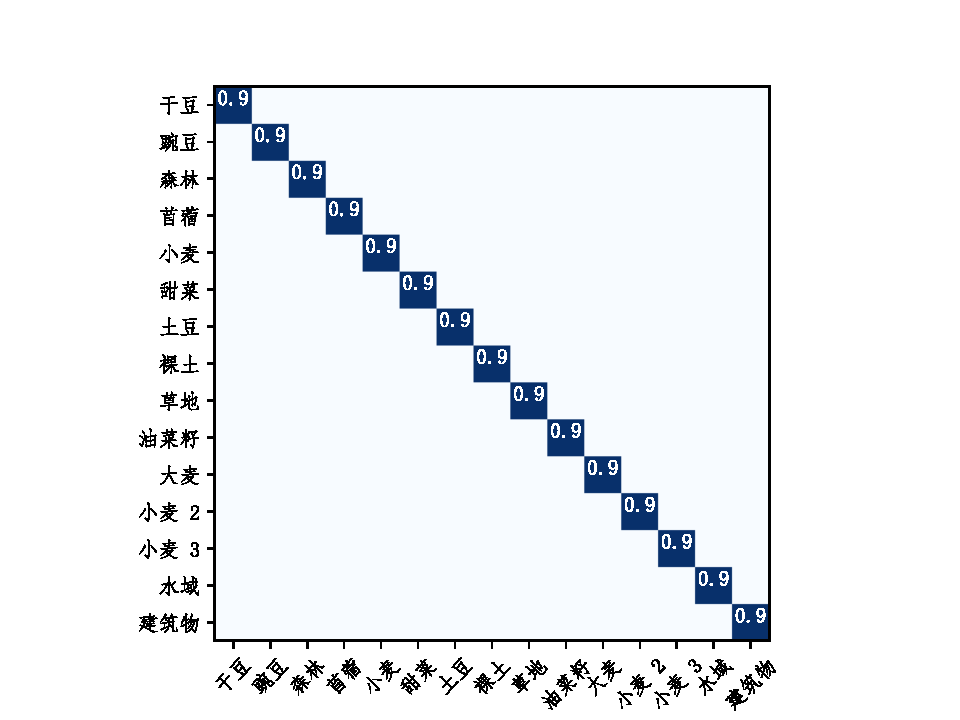
\includegraphics[width=10.04cm]{pic/chapter4/fle/noise_uniform.pdf}
  \caption{AIRSAR Flevoland数据10\%对称噪声转移矩阵}
  \label{fig:fle_noise_uniform}
\end{figure}

图\ref{fig:fle_res_4}展示了不同实验方法在10\%对称噪声类型下分类结果图。根据图\ref{fig:SVM}、图\ref{wishart}展示的SVM与Wishart分类器的分类结果,在大多数的类别中都存在着严重的错分情况,这可能是由于这两类分类器都无法有效地应对标签噪声的影响,错误的信息对分类规则噪声严重的负面影响,进而导致分类性能下降的现象。而图\ref{fig:CNN}展示的在交叉熵损失函数优化的CNN分类器的分类结果,可以看到小麦区域和干豆存在大量的错分情况,将小麦错分为水域,将干豆区域错分为土豆,这是因为这两类目标本身散射特性比较接近,容易造成错分,同时该分类模型并没有对标签噪声进行处理,模型过拟合学习到了错误的类别信息,导致错分的情况。图\ref{fig:RSL}展示了使用鲁棒分类方法的分类结果,可以看到大量连续错分的情况得到改善,但是在草地等区域出现了小块的错分样本,将草地错分为大麦,这可能是草地覆盖区域较小,又存在噪声的情况,导致有效的训练样本数量不足,同时RSL方法是将判断为噪声的样本直接丢弃也丢失了一部分信息,在这一块区域中的分类性能有限。图\ref{fig:BEL}与图\ref{fig:BEL_DP}均是本章提出的标签噪声下鲁棒性分类方法的分类结果图,从图中可以直观看出分类效果得到提升,错分的情况大大减少,仅有少数的错分情况,并且使用极化信息提取器后在油菜籽区域的错分情况也得到视觉上的改善,这也验证了本章方法的有效性。

\begin{figure}[ht]
  \subfloat[]{
    \label{fig:SVM}
    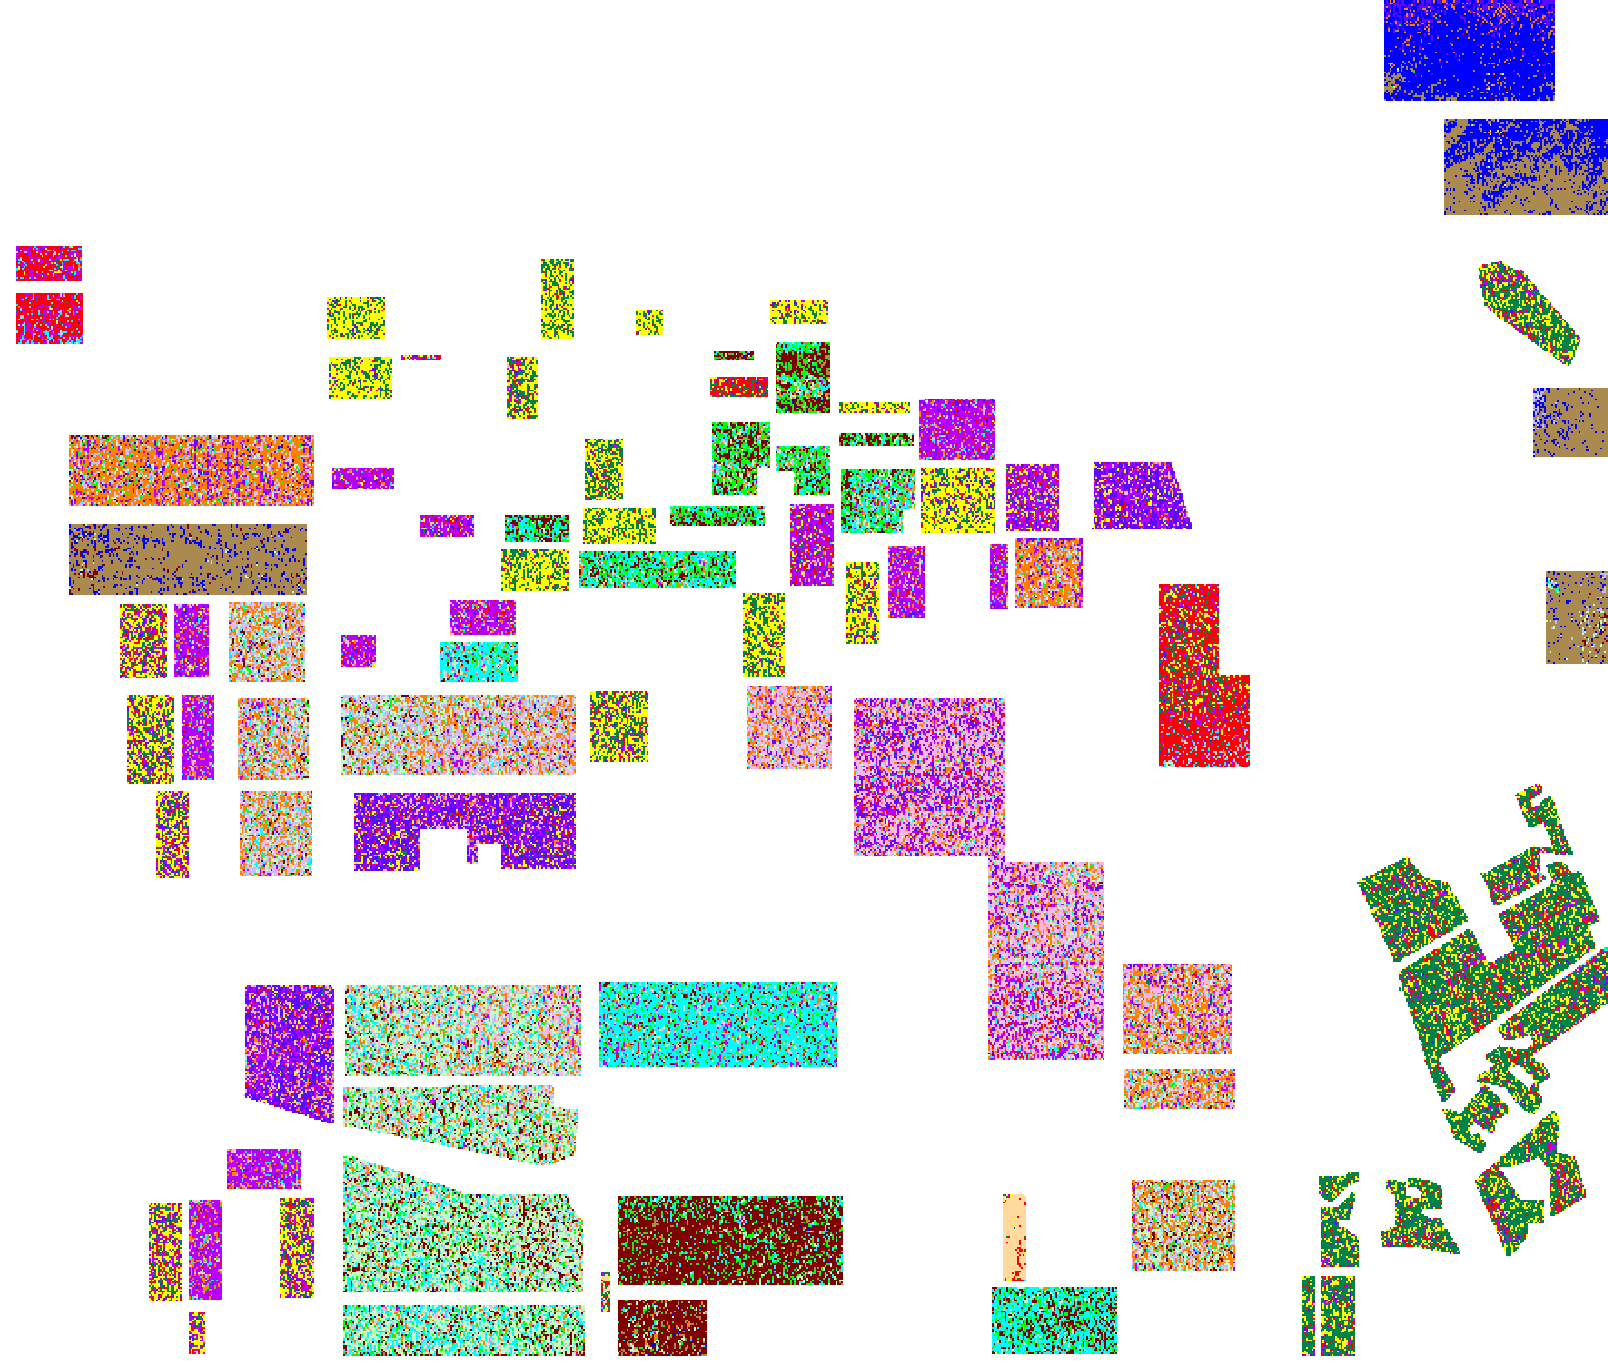
\includegraphics[width=4.04cm]{pic/chapter4/fle/SVM-10.png}
  }
  \subfloat[]{
    \label{fig:wishart}
    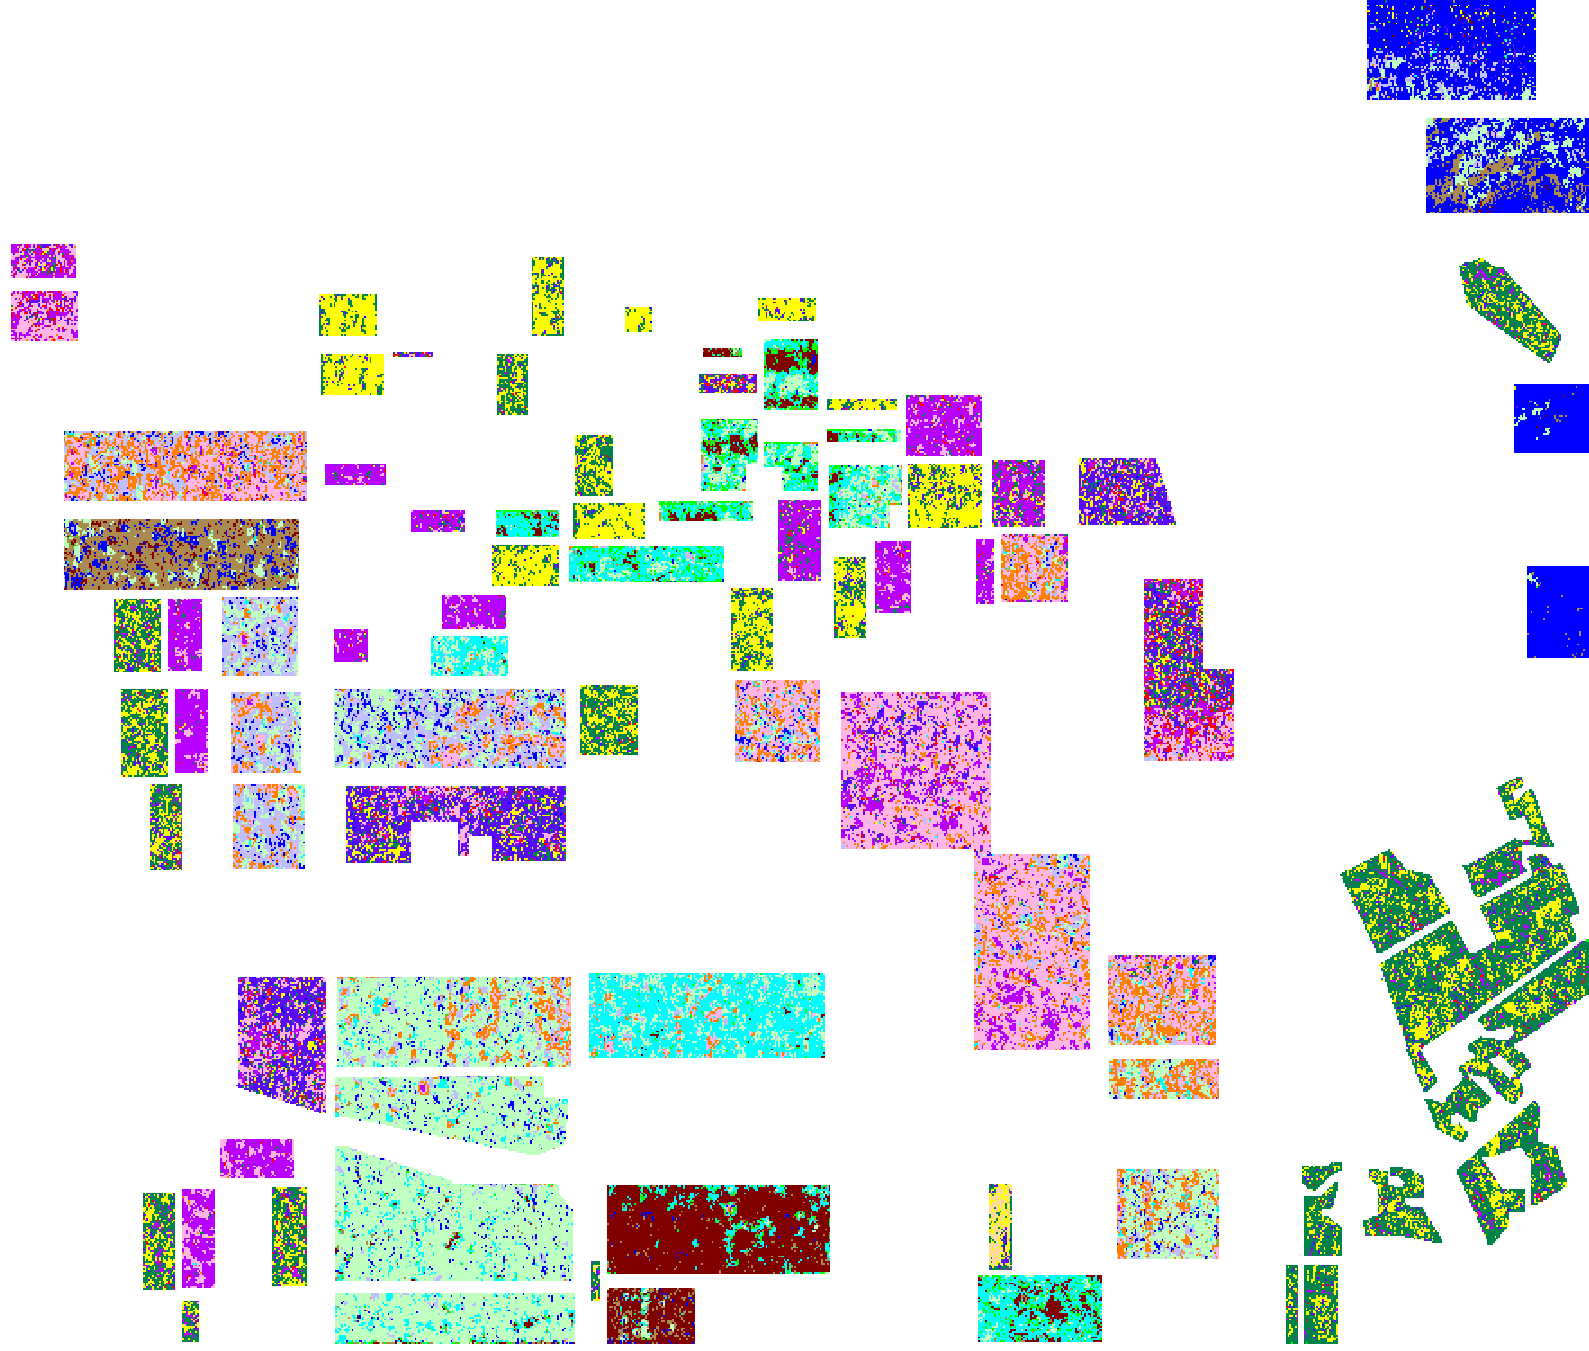
\includegraphics[width=4.04cm]{pic/chapter4/fle/Wishart-10.png}
  }
  \subfloat[]{
    \label{fig:CNN}
    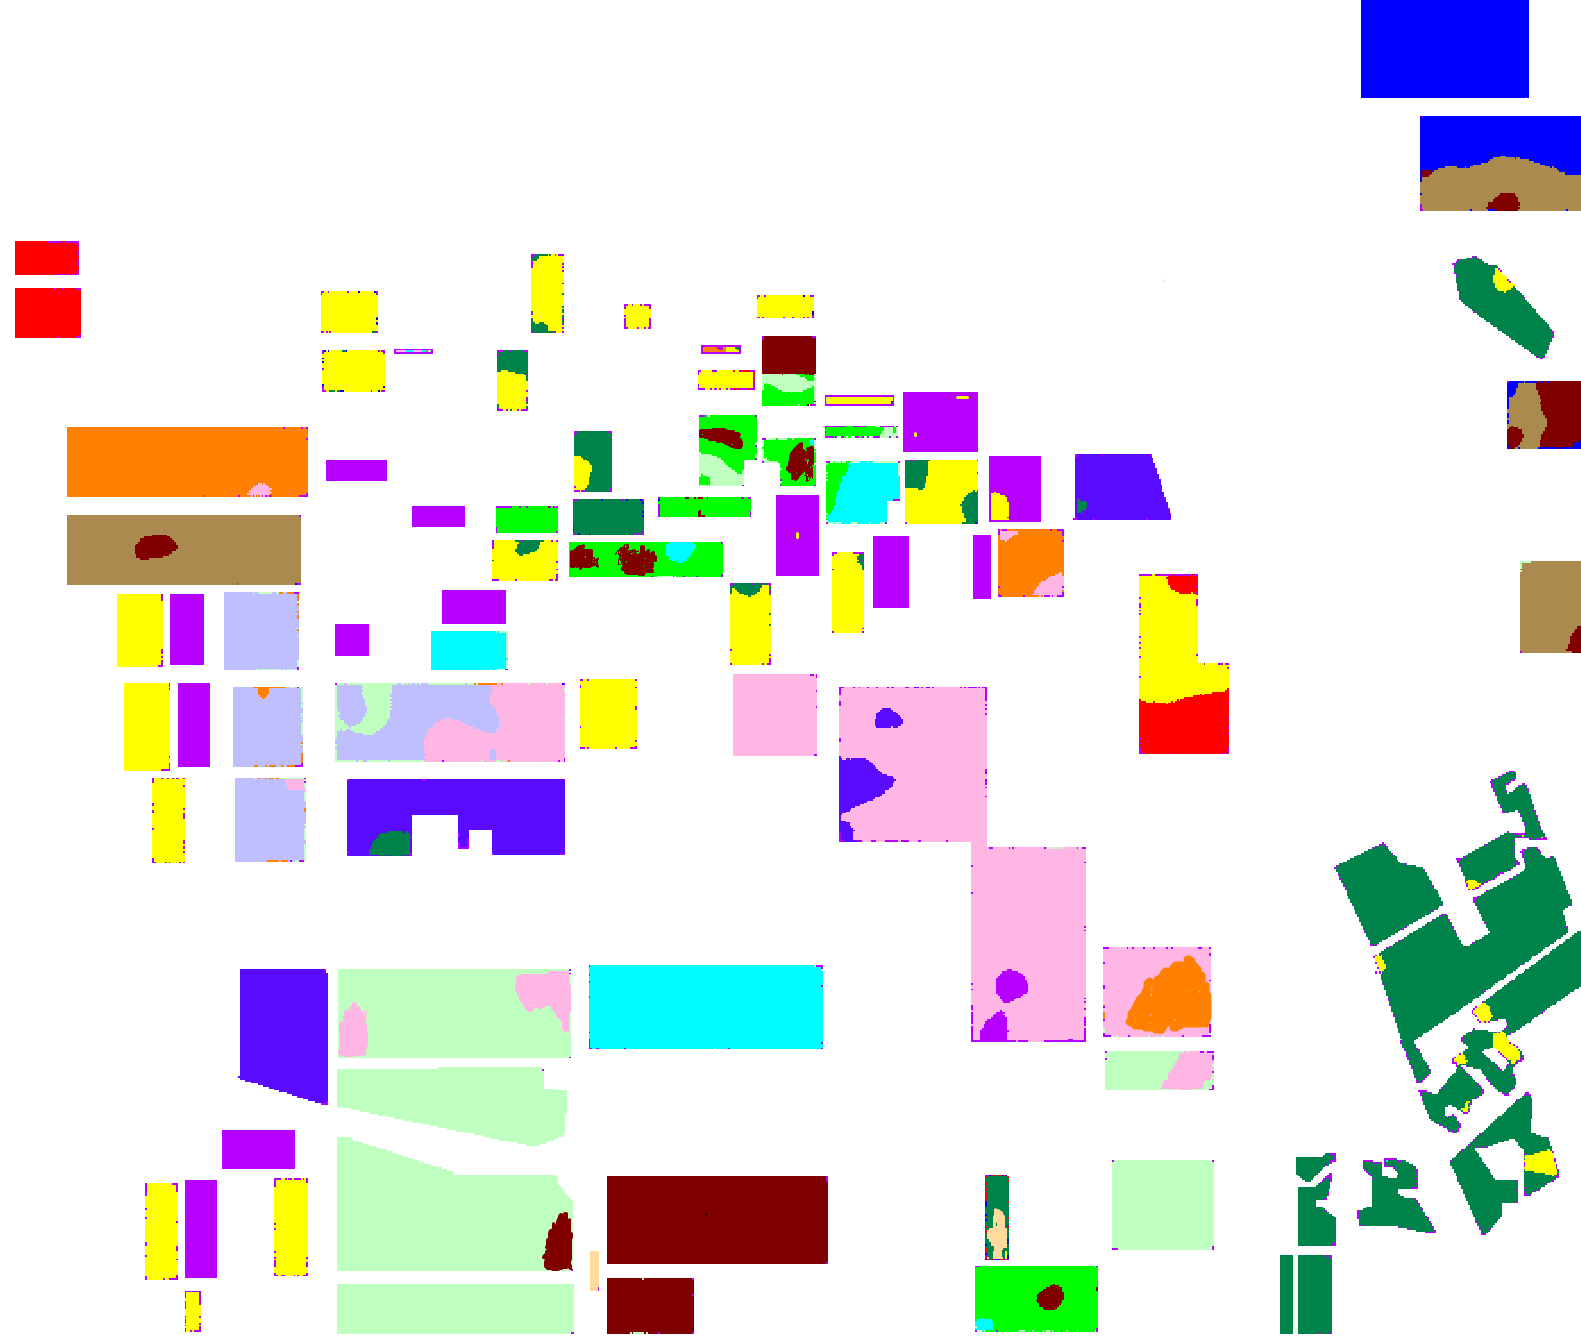
\includegraphics[width=4.04cm]{pic/chapter4/fle/CNN-10.png}
  }

  \subfloat[]{
    \label{fig:RSL}
    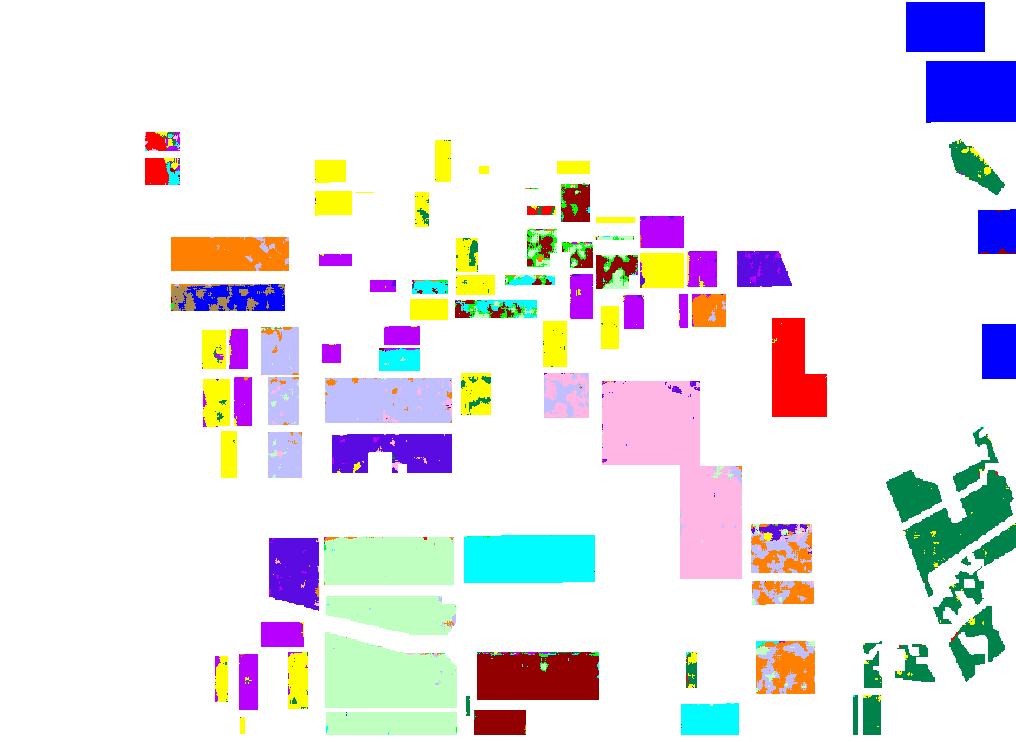
\includegraphics[width=4.04cm]{pic/chapter4/fle/RSL-10.png}
  }
  \subfloat[]{
    \label{fig:BEL}
    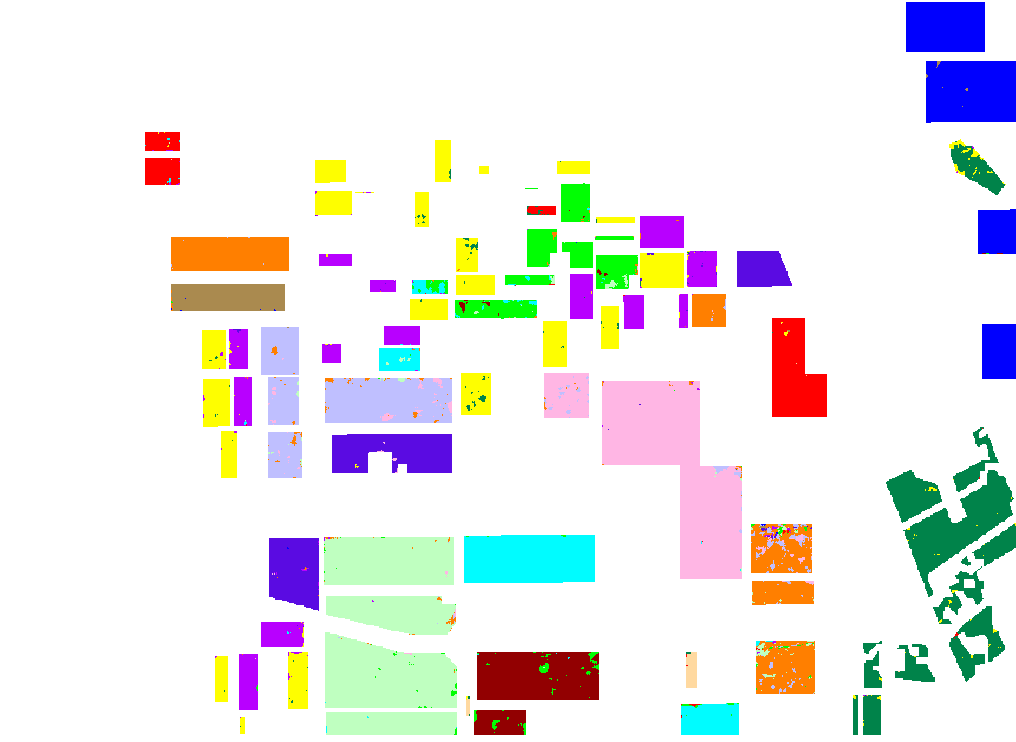
\includegraphics[width=4.04cm]{pic/chapter4/fle/BEL-10.png}
  }
  \subfloat[]{
    \label{fig:BEL_DP}
    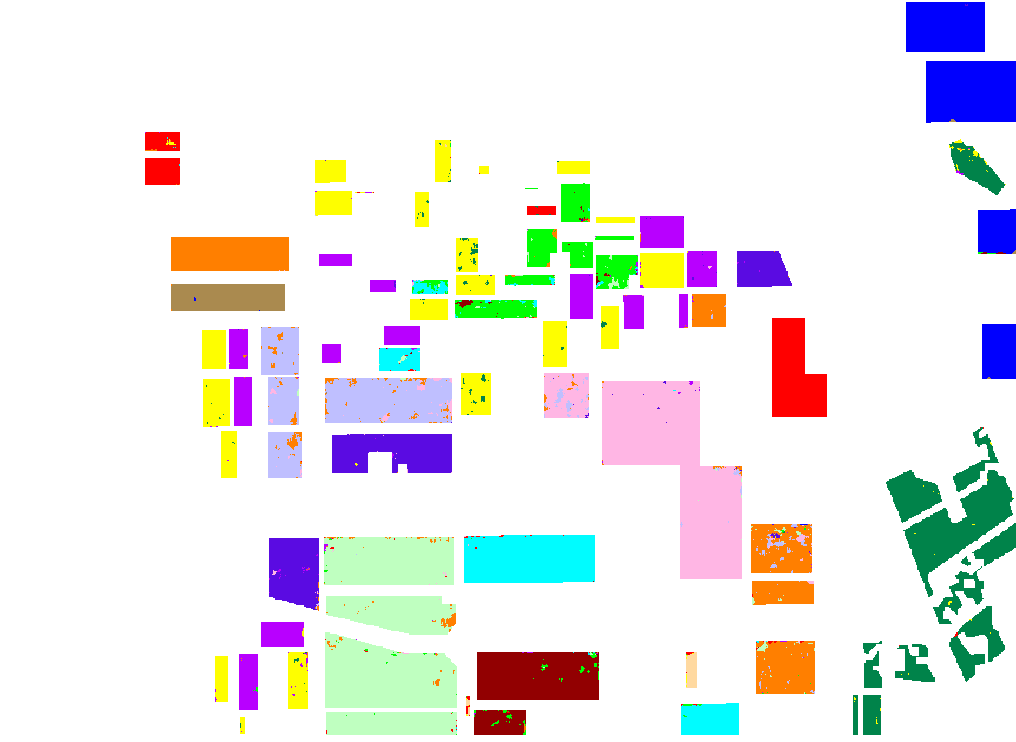
\includegraphics[width=4.04cm]{pic/chapter4/fle/BEL+DP-10.png}
  }

  \subfloat[]{
    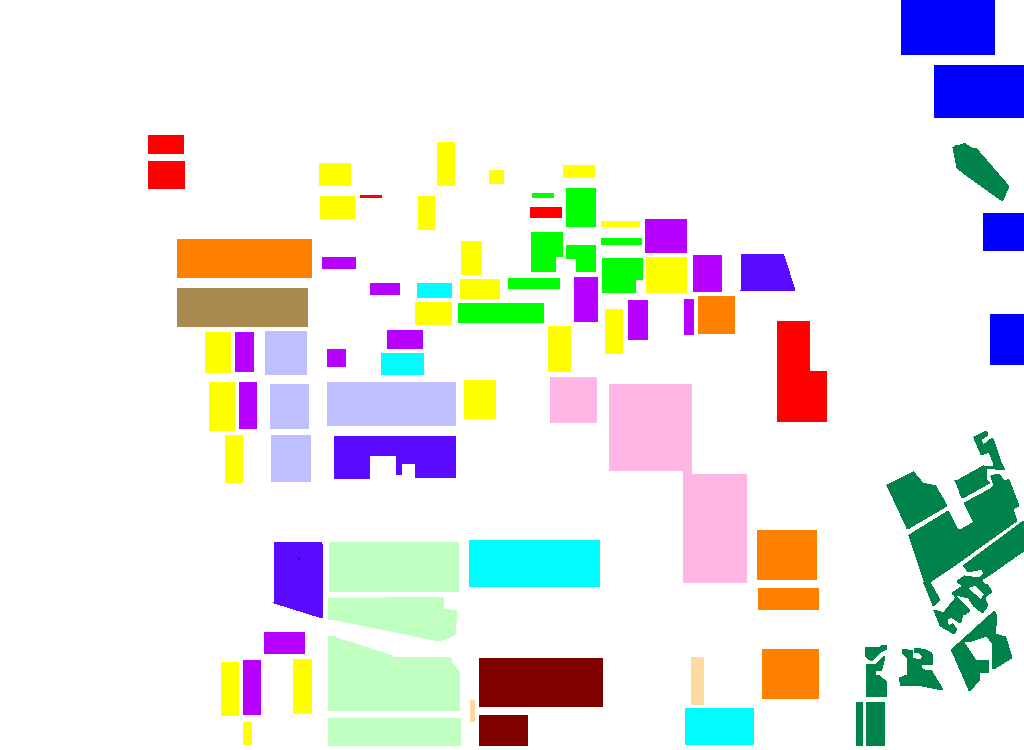
\includegraphics[width=4.04cm]{pic/chapter4/fle/gt.png}
  }
  \subfloat[]{
    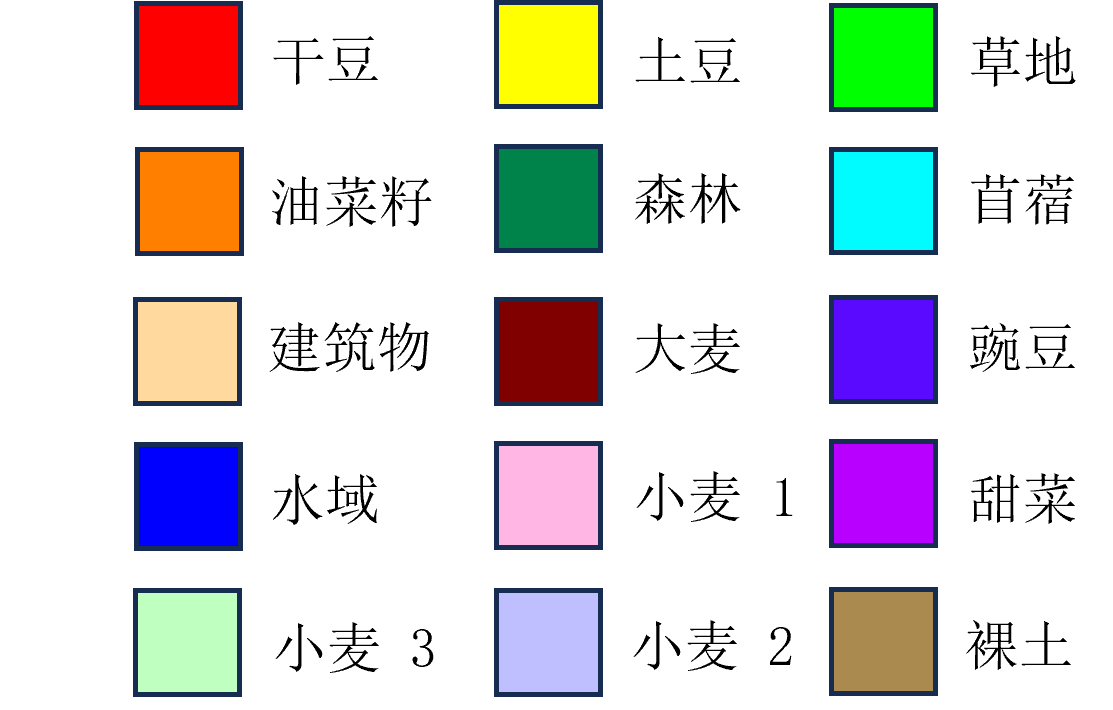
\includegraphics[width=4.04cm]{pic/chapter4/fle/label.png}
  }

  \caption{AIRSAR Flevoland地区数据对称标签噪声下分类可视化结果图。(a) SVM;(b)Wishart; (c) CNN; (d) RSL; (e) BEL; (f) BEL + DP; (g) 地面真值;(h) 颜色与类别对应关系}
  \label{fig:fle_res_4}
\end{figure}

表\ref{tab:fle_res_4}展示了不同分类方法在10\%对称标签噪声比例下的分类数值结果。SVM与Wishart分类方法由于无法有效应对标签噪声的影响,绝大多数类别的分类准确率都低于60\%,存在严重的错分的情况,总体分类准确率较低,分别为58.98\%和49.78\%。基于交叉熵损失的CNN分类器在油菜籽、干豆区域分类准确率较低,但是在其他类别上的分类准确率有了一定的提升,这可能是因为深度网络模型本身对于标签噪声的一定的鲁棒性能,会先学习特征简单的样本,再去学习错误的样本信息,总体分类准确率达到88.39\%。鲁棒性分类学习方法RSL由于对判断为噪声的样本进行了丢弃,在大多数类别上准确率取得了不错的成果,但是在建筑物区域的分类准确率较低,这可能是因为建筑物区域本身样本有限,添加噪声之后导致有效的训练样本不足,进而导致了在该类别上的分类准确率较低的情况。BEL与BEL+DP分类准确率相比于其他方法有了较大的提升,两个方法占据了所有类别和所有指标的最大值。BEL+DP方法在油菜籽、甜菜等区域中分类准确率稍低于BEL方法,不足1\%的差距,但是在建筑物、甜菜等区域中的分类准确率高于BEL方法超过1\%,验证了极化信息表征对该场景下性能提升的有效性。通过以上分析证明,本章提出的BEL方法对标签噪声的有效性与优越性。

\begin{table}[ht!]
  \begin{tabular}{cccccccc}
    \toprule[1.5bp]
    序号                        & 类别    & SVM   & Wishart & CNN   & RSL            & BEL            & BEL + DP       \\
    \midrule[0.75bp]
    1                         & 建筑物   & 37.26 & 32.64   & 65.07 & 79.52          & 86.38          & \textbf{87.75} \\
    2                         & 油菜籽   & 31.35 & 15.58   & 33.32 & 66.64          & \textbf{92.01} & 90.27          \\
    3                         & 甜菜    & 74.17 & 9.87    & 77.49 & \textbf{99.01} & 95.67          & 97.28          \\
    4                         & 干豆    & 14.61 & 14.02   & 58.6  & 74.63          & \textbf{96.92} & 96.62          \\
    5                         & 豌豆    & 50.2  & 22.9    & 79.68 & 96.39          & \textbf{99.11} & 98.8           \\
    6                         & 森林    & 66.31 & 41.52   & 83.57 & 94.34          & 96.8           & \textbf{97.7}  \\
    7                         & 苜蓿    & 62.92 & 17.71   & 59.63 & 80.53          & 96.19          & \textbf{98}    \\
    8                         & 土豆    & 53.54 & 26.89   & 72.74 & 83.1           & 95.49          & \textbf{98.42} \\
    9                         & 裸土    & 64.25 & 11.36   & 80.46 & \textbf{95.05} & 91.02          & 93.12          \\
    10                        & 草地    & 19.64 & 17.27   & 55    & 80.43          & 87.65          & \textbf{91.66} \\
    11                        & 大麦    & 80.89 & 10.48   & 79.28 & 89.43          & 96.26          & \textbf{97.49} \\
    12                        & 水域    & 76.9  & 59.9    & 49.51 & 79.32          & 97.37          & \textbf{99.85} \\
    13                        & 小麦 1  & 59.13 & 40.18   & 82.51 & 91.83          & \textbf{97.71} & 97.23          \\
    14                        & 小麦 2  & 45.27 & 46.52   & 64.23 & 80.16          & \textbf{94.82} & 94.22          \\
    15                        & 小麦 3  & 75.74 & 43.69   & 73.65 & \textbf{98.85} & 97.05          & 98.06          \\
    \midrule[0.75bp]
    \multicolumn{2}{c}{OA}    & 58.98 & 49.78 & 69.83   & 86.13 & 95.25          & \textbf{96.36}                  \\
    \multicolumn{2}{c}{AA}    & 54.15 & 27.36 & 67.64   & 85.94 & 94.7           & \textbf{95.76}                  \\
    \multicolumn{2}{c}{Kappa} & 56.02 & 47.16 & 67.56   & 85.12 & 95.47          & \textbf{96.58}                  \\
    \bottomrule[1.5bp]
  \end{tabular}
  \caption{AIRSAR Flevoland地区数据对称标签噪声下分类数值结果(\%)}
  \label{tab:fle_res_4}
\end{table}

\subsubsection{非对称标签实验}
图\ref{fig:fle_noise_random}展示了10\%噪声比例下非对称标签噪声的噪声转移矩阵,每个类别正确标记的概率为90\%,10\%的标签噪声随机映射到另外的一个类别中。
\begin{figure}[ht!]
  \centering
  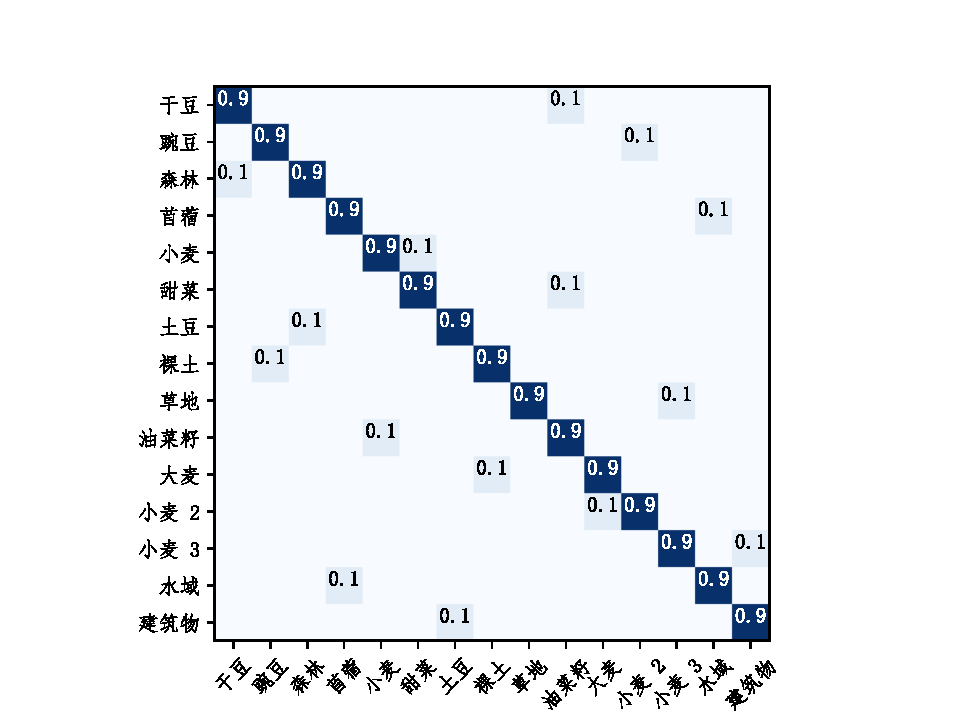
\includegraphics[width=10.04cm]{pic/chapter4/fle/noise_random.pdf}
  \caption{AIRSAR Flevoland数据10\%非对称噪声转移矩阵}
  \label{fig:fle_noise_random}
\end{figure}

%TODO:
图\ref{fig:fle_random}展示了10\%非对称标签噪声下不同对比方法的分类结果。图\ref{fig:SVM_random}与图\ref{fig:wishart_random}依然存在大量的错分情况,并且区域内部存在大量斑点状的错误区域。图\ref{fig:CNN_random}展示了交叉熵损失下的CNN分类结果,由于训练集中油菜籽区域部分像素被标记为小麦,导致在分类结果中也存在相同的错分情况,这表明该分类方法在错误标记训练集上过拟合,学习了错误的分类规则。图\ref{fig:RSL_random}展示了RSL方法的分类结果,可以看出在油菜籽、大麦区域依然存在大块连续的错分区域,将大麦错分为苜蓿,这是因为RSL对大量的错误样本过滤性能有限。图\ref{fig:BEL_random}与图\ref{fig:BEL_DP_random}展示了BEL与BEL+DP方法的分类结果,可以看到由于对称噪声标签的影响,在小麦、林地、油菜籽区域出现了一定的错分情况,但是在其他大部分区域分类结果较平滑,错分样本较少,以上结果证明了本章方法在非对称噪声标签下的有效性与优越性。

\begin{figure}[ht!]
  \subfloat[]{
    \label{fig:SVM_random}
    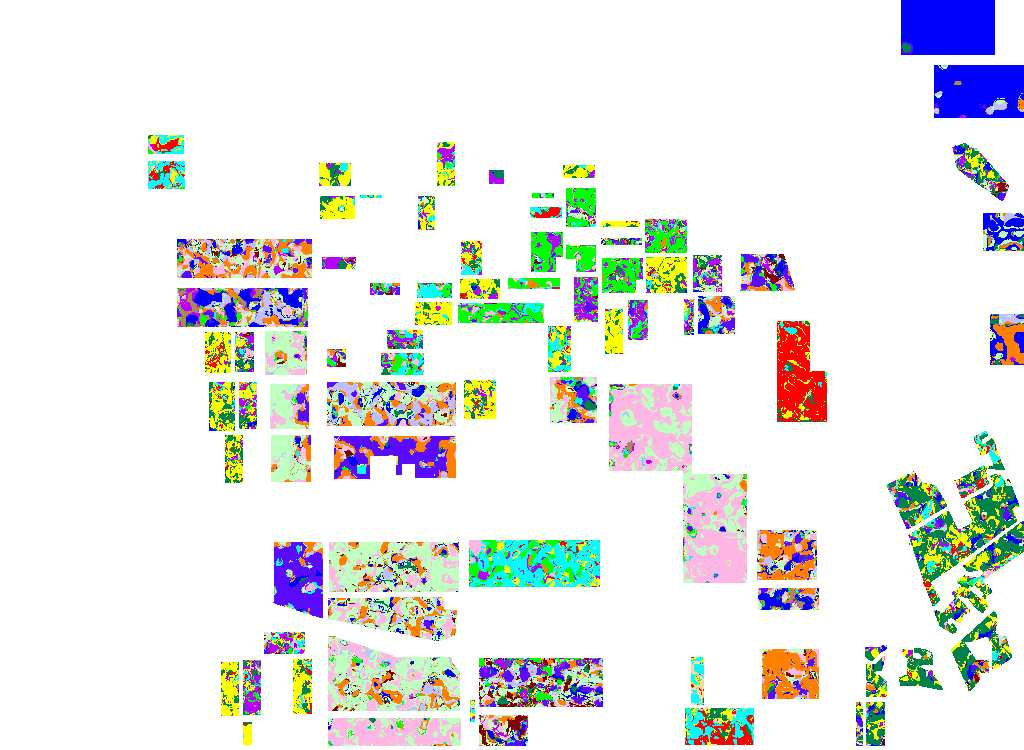
\includegraphics[width=4.04cm]{pic/chapter4/fle/SVM_random.png}
  }
  \subfloat[]{
    \label{fig:wishart_random}
    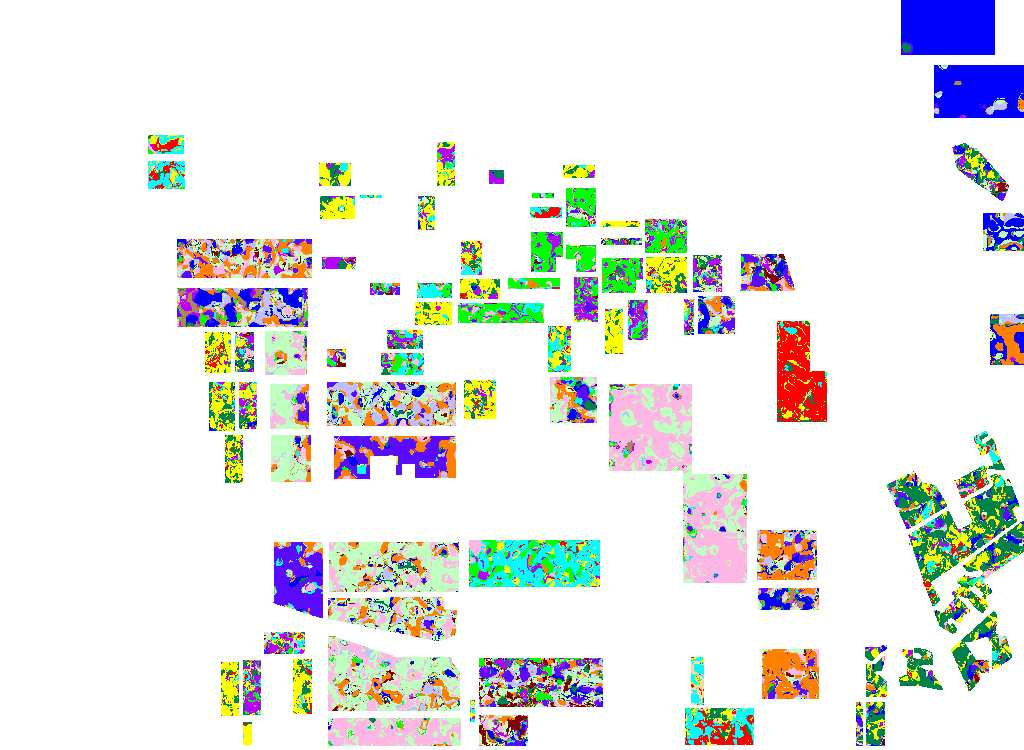
\includegraphics[width=4.04cm]{pic/chapter4/fle/Wishart_random.png}
  }
  \subfloat[]{
    \label{fig:CNN_random}
    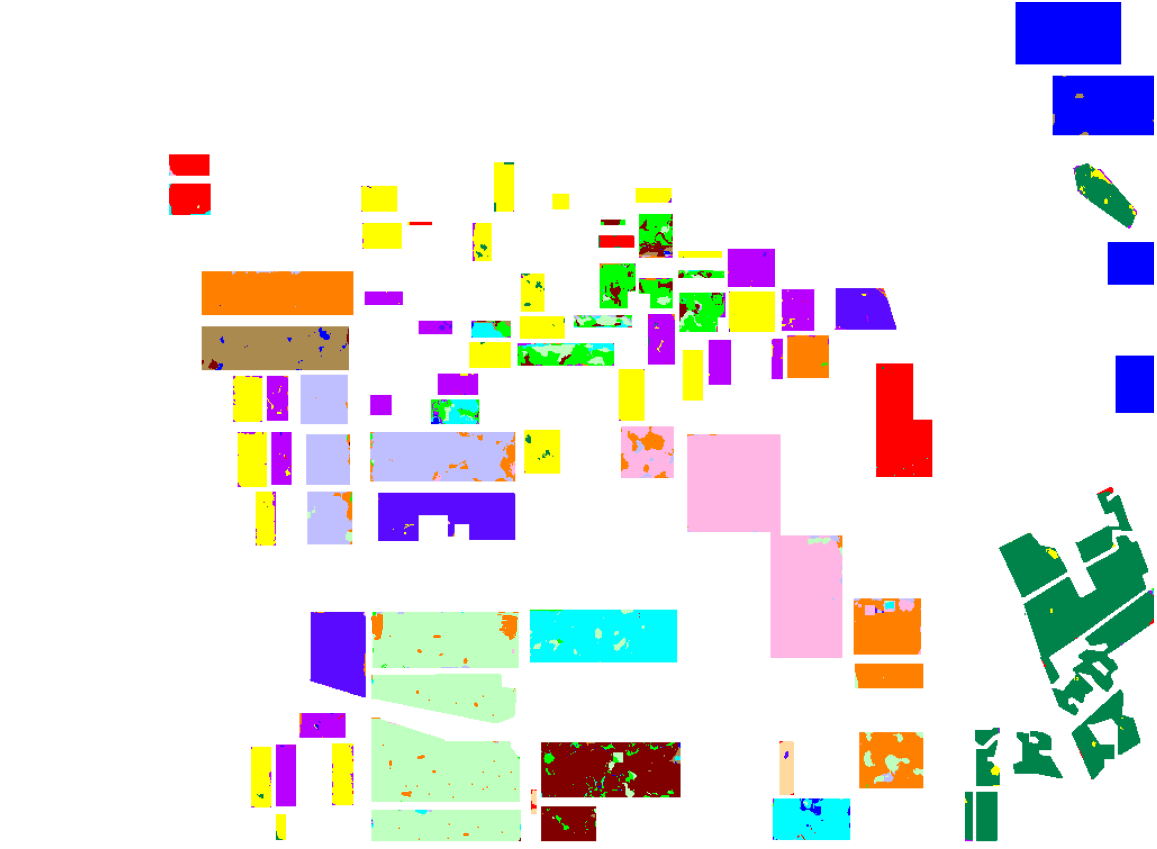
\includegraphics[width=4.04cm]{pic/chapter4/fle/CNN_random.png}
  }

  \subfloat[]{
    \label{fig:RSL_random}
    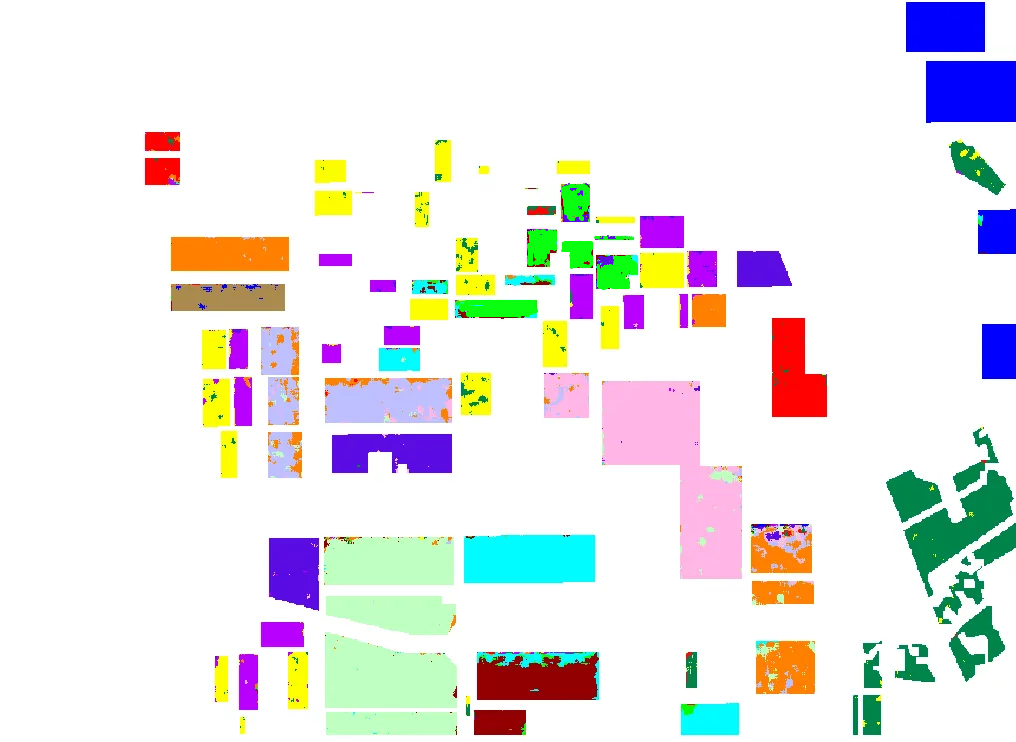
\includegraphics[width=4.04cm]{pic/chapter4/fle/RSL_random.png}
  }
  \subfloat[]{
    \label{fig:BEL_random}
    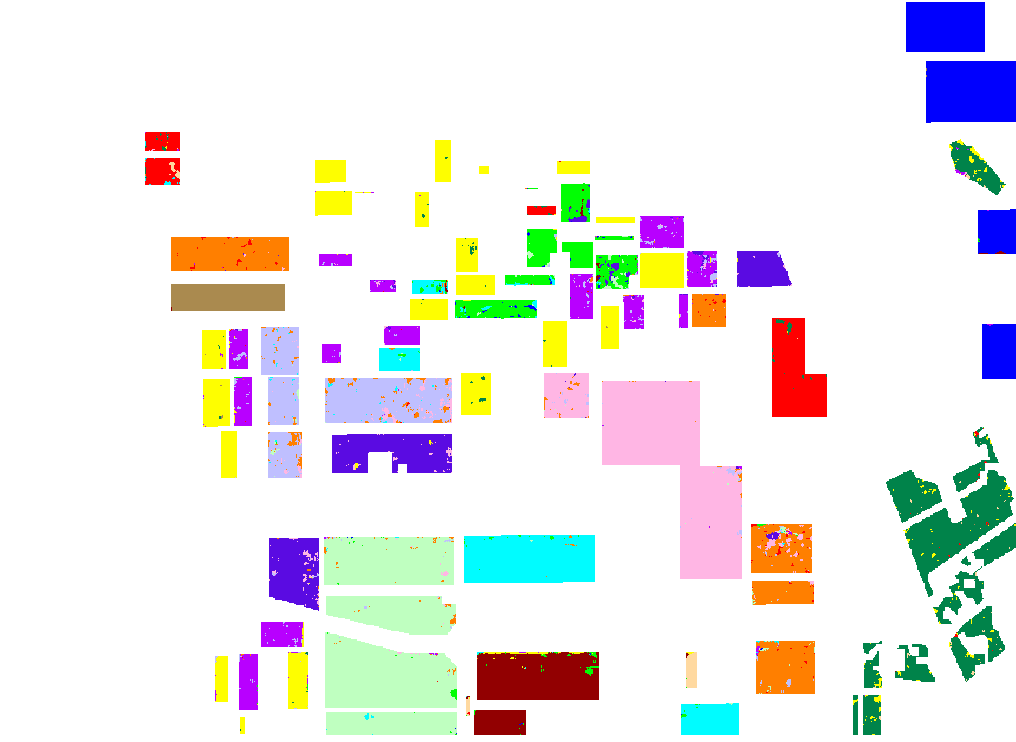
\includegraphics[width=4.04cm]{pic/chapter4/fle/BEL_random.png}
  }
  \subfloat[]{
    \label{fig:BEL_DP_random}
    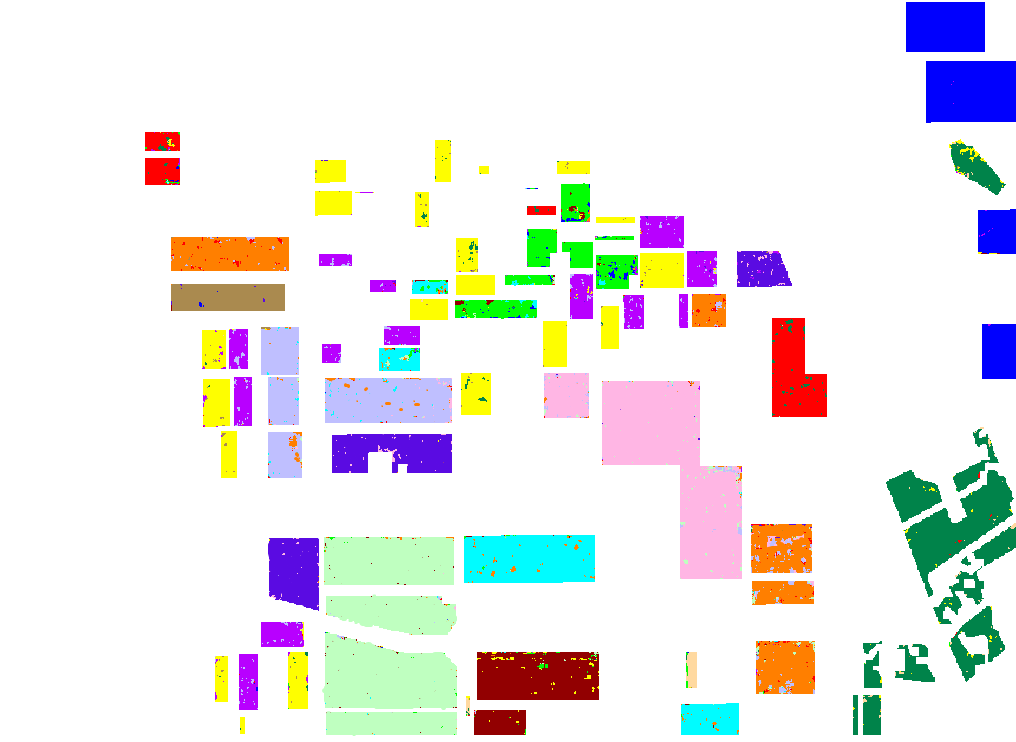
\includegraphics[width=4.04cm]{pic/chapter4/fle/BEL+DP_random.png}
  }

  \subfloat[]{
    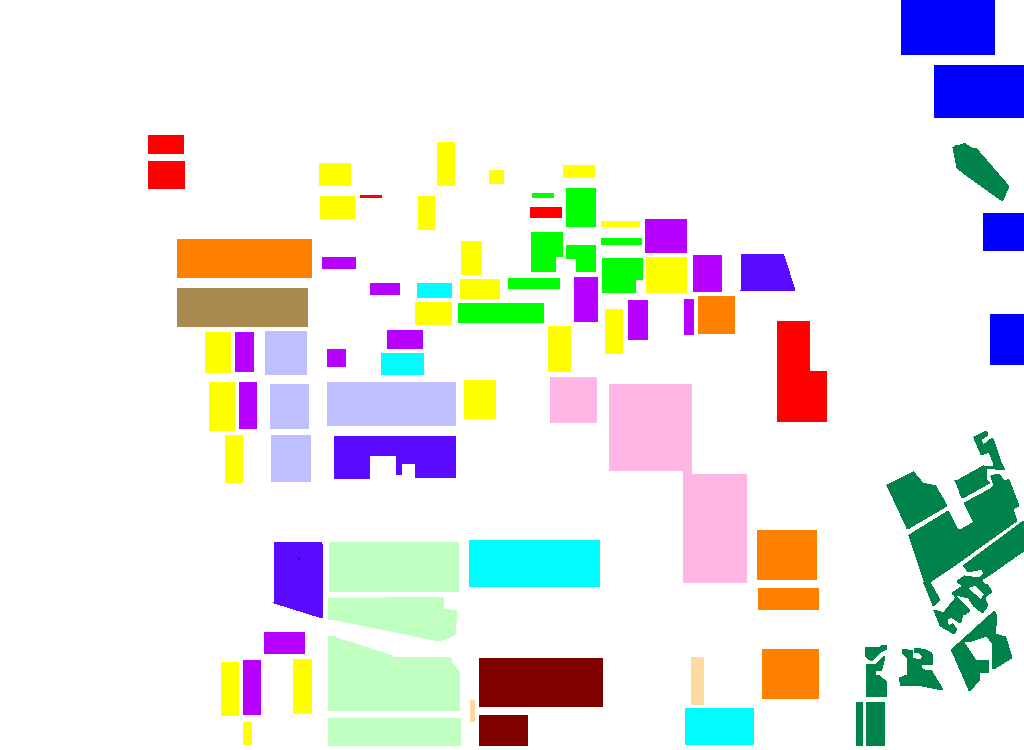
\includegraphics[width=4.04cm]{pic/chapter4/fle/gt.png}
  }
  \subfloat[]{
    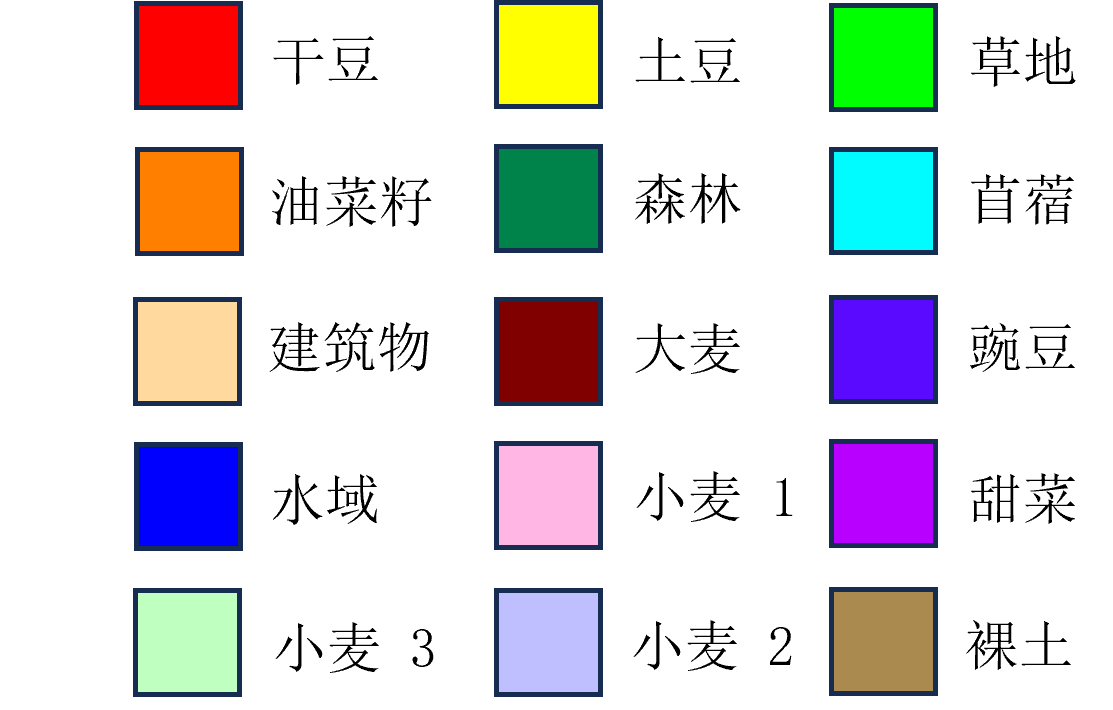
\includegraphics[width=4.04cm]{pic/chapter4/fle/label.png}
  }

  \caption{AIRSAR Flevoland地区数据非对称标签噪声下分类可视化结果图。(a) SVM;(b)Wishart; (c) CNN; (d) RSL; (e) BEL; (f) BEL + DP; (g) 地面真值;(h) 颜色与类别对应关系}
  \label{fig:fle_random}
\end{figure}


表\ref{tab:fle_res_random}展示了各对比方法在非对称标签噪声下的分类数值结果。SVM与Wishart作为经典的极化SAR分类方法,在非对称标签标签噪声下分类效果不理想,总体准确率分别为56.48\%与50.32\%,这是因为基于SVM与Wishart的方法分类器模型简单,无法鉴别标签噪声的错误信息。基于交叉熵损失的CNN方法虽然整体有了提升,但是在建筑物区域准确率仅为42.28\%,这是因为CNN也不具备对标签噪声的鲁棒性能,会学习到错误的分类准则。除了干豆、水域、大麦三个区域略低于RSL方法,本章方法在其他指标上均取得了最高值,尤其是建筑物区域获得了较大的提升,反映了本章提出的方法是有效且优越的。

\begin{table}[ht!]
  \caption{AIRSAR Flevoland地区数据非对称标签噪声下分类数值结果(\%)}
  \label{tab:fle_res_random}
  \begin{tabular}{cccccccc}
    \toprule[1.5bp]
    序号                        & 类别    & SVM   & Wishart & CNN   & RSL            & BEL            & BEL + DP       \\
    \midrule[0.75bp]
    1                         & 建筑物   & 31.73 & 31.56   & 42.28 & 46.24          & 91.09          & \textbf{96.16} \\
    2                         & 油菜籽   & 33.76 & 18.23   & 61.25 & 82.77          & \textbf{92.34} & 92.19          \\
    3                         & 甜菜    & 73.98 & 10.56   & 74.86 & 95.23          & 96.68          & \textbf{97.92} \\
    4                         & 干豆    & 16.23 & 12.97   & 85.41 & \textbf{96.8}  & 91.01          & 94.6           \\
    5                         & 豌豆    & 48.34 & 24.56   & 87.73 & 95.62          & 97.86          & \textbf{97.39} \\
    6                         & 森林    & 64.28 & 40.08   & 82.19 & 91.36          & 96.68          & \textbf{97.96} \\
    7                         & 苜蓿    & 60.72 & 18.23   & 79.2  & 79.8           & 94.43          & \textbf{96.04} \\
    8                         & 土豆    & 52.01 & 22.14   & 81.69 & \textbf{95.9}  & 95.68          & 94.41          \\
    9                         & 裸土    & 64.58 & 14.2    & 81.32 & 98.04          & 94.01          & \textbf{99.39} \\
    10                        & 草地    & 21.33 & 19.32   & 77.84 & 64.59          & 92.98          & \textbf{92.4}  \\
    11                        & 大麦    & 78.89 & 9.47    & 76.23 & 59.39          & 89.52          & \textbf{97.24} \\
    12                        & 水域    & 75.42 & 58.14   & 68.04 & \textbf{98.2}  & 97.35          & 97.7           \\
    13                        & 小麦 1  & 57.6  & 42.18   & 80.37 & \textbf{94.83} & 93.97          & 93.87          \\
    14                        & 小麦 2  & 44.32 & 44.25   & 65.17 & 86.95          & 83.83          & \textbf{91.55} \\
    15                        & 小麦 3  & 74.36 & 45.84   & 70.35 & 94.2           & 94.72          & \textbf{98.12} \\
    \midrule[0.75bp]
    \multicolumn{2}{c}{OA}    & 56.48 & 50.32 & 75.28   & 89.88 & 93.82          & \textbf{96.52}                  \\
    \multicolumn{2}{c}{AA}    & 53.17 & 27.45 & 74.26   & 88.91 & 91.48          & \textbf{95.79}                  \\
    \multicolumn{2}{c}{Kappa} & 54.59 & 48.03 & 73.96   & 88.94 & 93.26          & \textbf{95.22}                  \\
    \bottomrule[1.5bp]
  \end{tabular}
\end{table}

图\ref{fig:fle_noise}展示了各个对比方法在两种噪声类型下分类准确率随着噪声比例的变化情况。从图中可以看出,随着标签噪声比例增加,各个方法分类准确率呈现不同程度的下降。在对称标签噪声下,SVM、Wishart、CNN这三种未考虑噪声标签影响的分类方法随着噪声比例增加下降幅度较快,在方法的分类准确率不高的情况下,从10\%噪声比例至50\%分别下降了22.70\%、13.91\%和18.40\%,表明了标签噪声带来的错误信息对分类任务形成了较大的影响。对于RSL方法,从10\%噪声比例至50\%分类准确率下降了10.59\%,下降幅度相对较小,但是在50\%噪声比例下分类准确率低于80\%,表明该方法对高比例噪声标签的鲁棒性能有限。BEL与BEL+DP方法从10\%噪声比例至50\%分类准确率分别下降了9.9\%和8.69\%,准确率下降幅度均小于10\%,且在50\%噪声比例下准确率依然均在85\%以上。从图中还可以看出,相同噪声比例下,非对称噪声源下的分类准确率要明显低于对称噪声源,SVM、Wishart分类方法的最差分类准确率已经低于30\%,RSL方法的最差分类准确率降到了54.32\%,本章分类方法降到了56.20\%。尽管大面积的错误标记样本严重影响了模型分类规则,导致无法根据损失判定噪声概率,但是本章方法的分类准确率指标依然高于对比方法。以上结果证明了本章方法对不同噪声类型、不同噪声比例均具有良好的鲁棒性能。

\begin{figure}[ht!]
  \subfloat[]{
    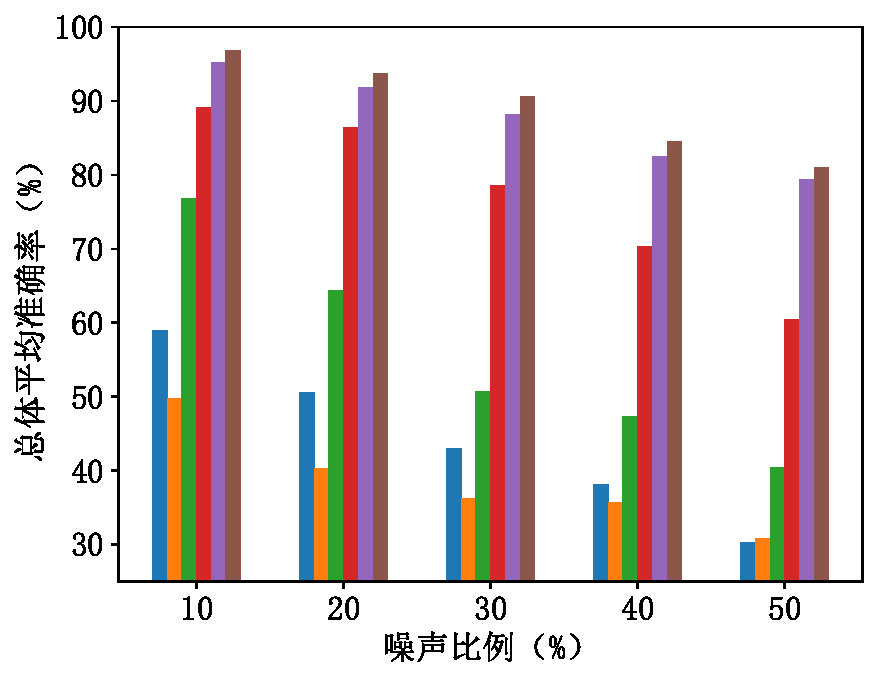
\includegraphics[width=6.24cm]{pic/chapter4/fle/noise_sy.pdf}
  }
  \subfloat[]{
    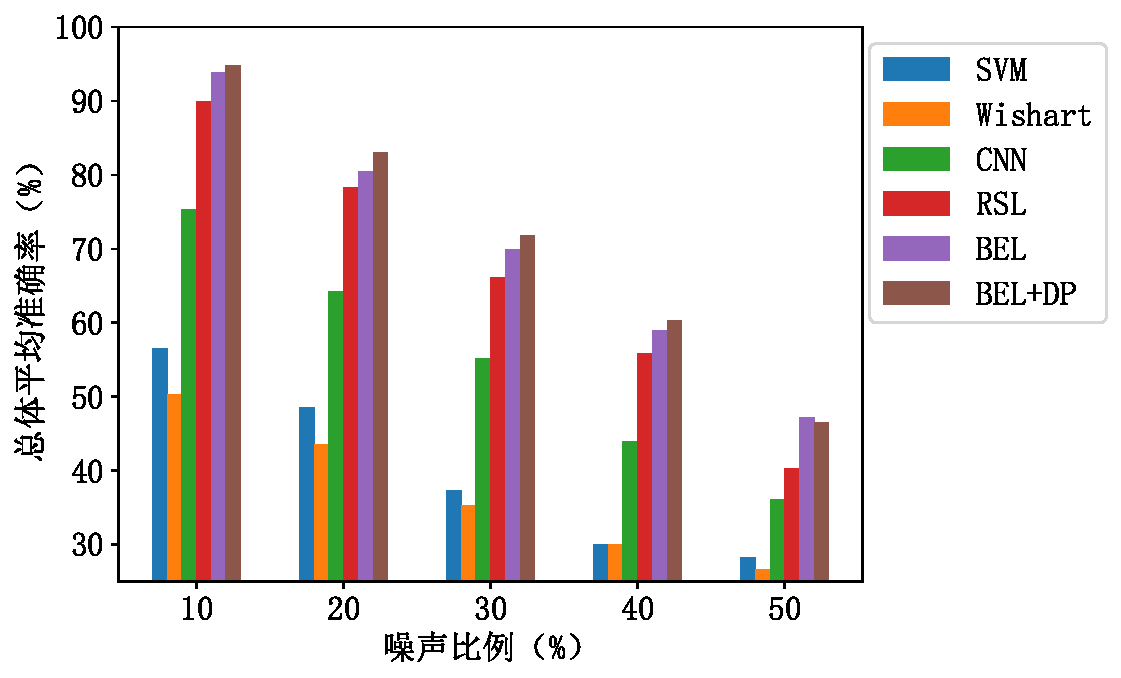
\includegraphics[width=8.04cm]{pic/chapter4/fle/noise_in.pdf}
  }
  \caption{AIRSAR Flevoland地区数据不同噪声比例下分类准确率结果。(a) 对称噪声源; (b) 非对称噪声源}
  \label{fig:fle_noise}
\end{figure}

\subsection{E-SAR Oberpfaffenhofen数据实验}
\subsubsection{对称标签实验}
图\ref{fig:ober_noise_uniform}展示了10\%噪声比例下对称标签噪声的噪声转移矩阵,每个类别正确标记的概率为90\%,10\%的标签噪声均匀地分布在其他类别中。
\begin{figure}[ht!]
  \centering
  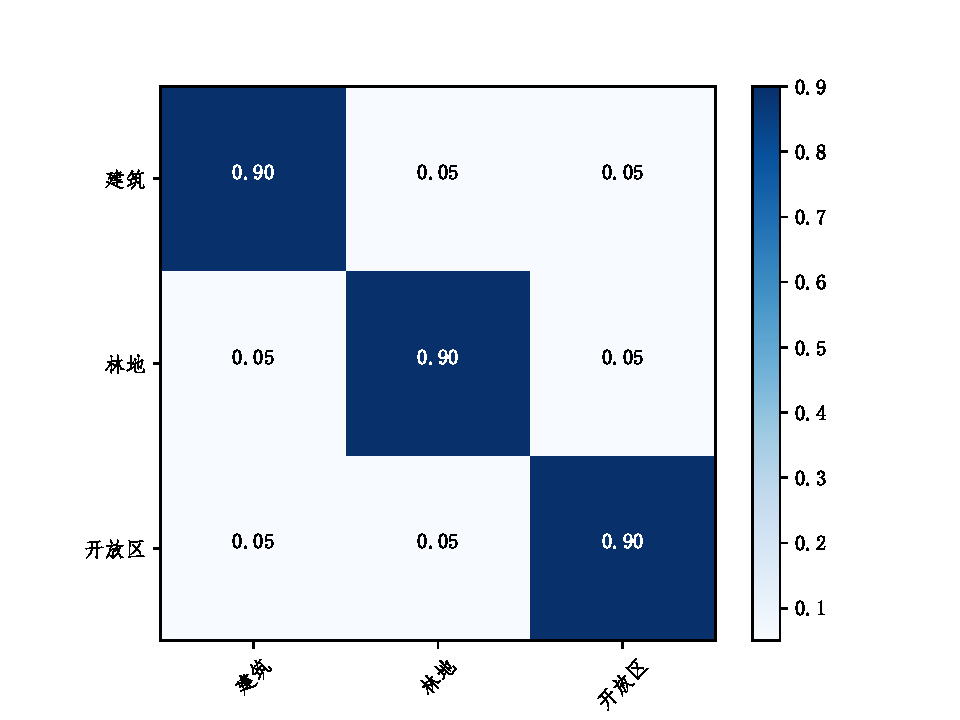
\includegraphics[width=10.04cm]{pic/chapter4/ober/noise_uniform.pdf}
  \caption{E-SAR Oberpfaffenhofen数据10\%对称噪声转移矩阵}
  \label{fig:ober_noise_uniform}
\end{figure}

图\ref{fig:ober_res_random}展示了不同分类方法在10\%对称标签噪声条件下的分类可视化图。根据图\ref{fig:ober_Wishart}与\ref{fig:ober_SVM}展示的Wishart与SVM的分类结果,可以看出分类效果较差,尤其是在林地、建筑区域存在大量的错分样本,将建筑物区域错分为开放区,将林地区域错分为建筑区域,一方面是因为Wishart与SVM分类方法的分类性能有限,对散射特性复杂的极化SAR数据分类结果不理想,另一方面是因为将错误的标签噪声信息归为学习规则之一,学习到错误的分类规则,导致分类性能的进一步下降。根据图\ref{fig:ober_CNN}展示的在交叉熵损失函数优化的CNN分类器的分类结果,可以看到相比于SVM与Wishart的分类效果有了一定的提升,但是依然存在着错误分类情况,主要是将建筑物区域分类为开放区,这是因为建筑物区域的散射特性差异大,并且交叉上损失函数的CNN会学习错误的标签信息,造成在训练集上过拟合,进而导致在测试集错分的情况。根据图\ref{fig:ober_RSL}展示的RSL方法的分类结果,经过对噪声标签概率估计后过滤可能是错误的信息的操作,可以看到分类效果直观好于CNN方法,但是依然在建筑区、林地区域存在少量的错误块,这可能是因为RSL直接丢弃了错误的样本,丢失了训练样本中的数据分布特征,导致分类性能有限。图\ref{fig:ober_BEL}与图\ref{fig:ober_BEL_DP}展示的BEL与BEL+DP方法的分类结果,可以看到错分情况得到改善,在类别区域内部更加平滑,错分块数量减少,证明了本章方法的有效性与优越性。
\begin{figure}[ht!]
  \subfloat[]{
    \label{fig:ober_Wishart_}
    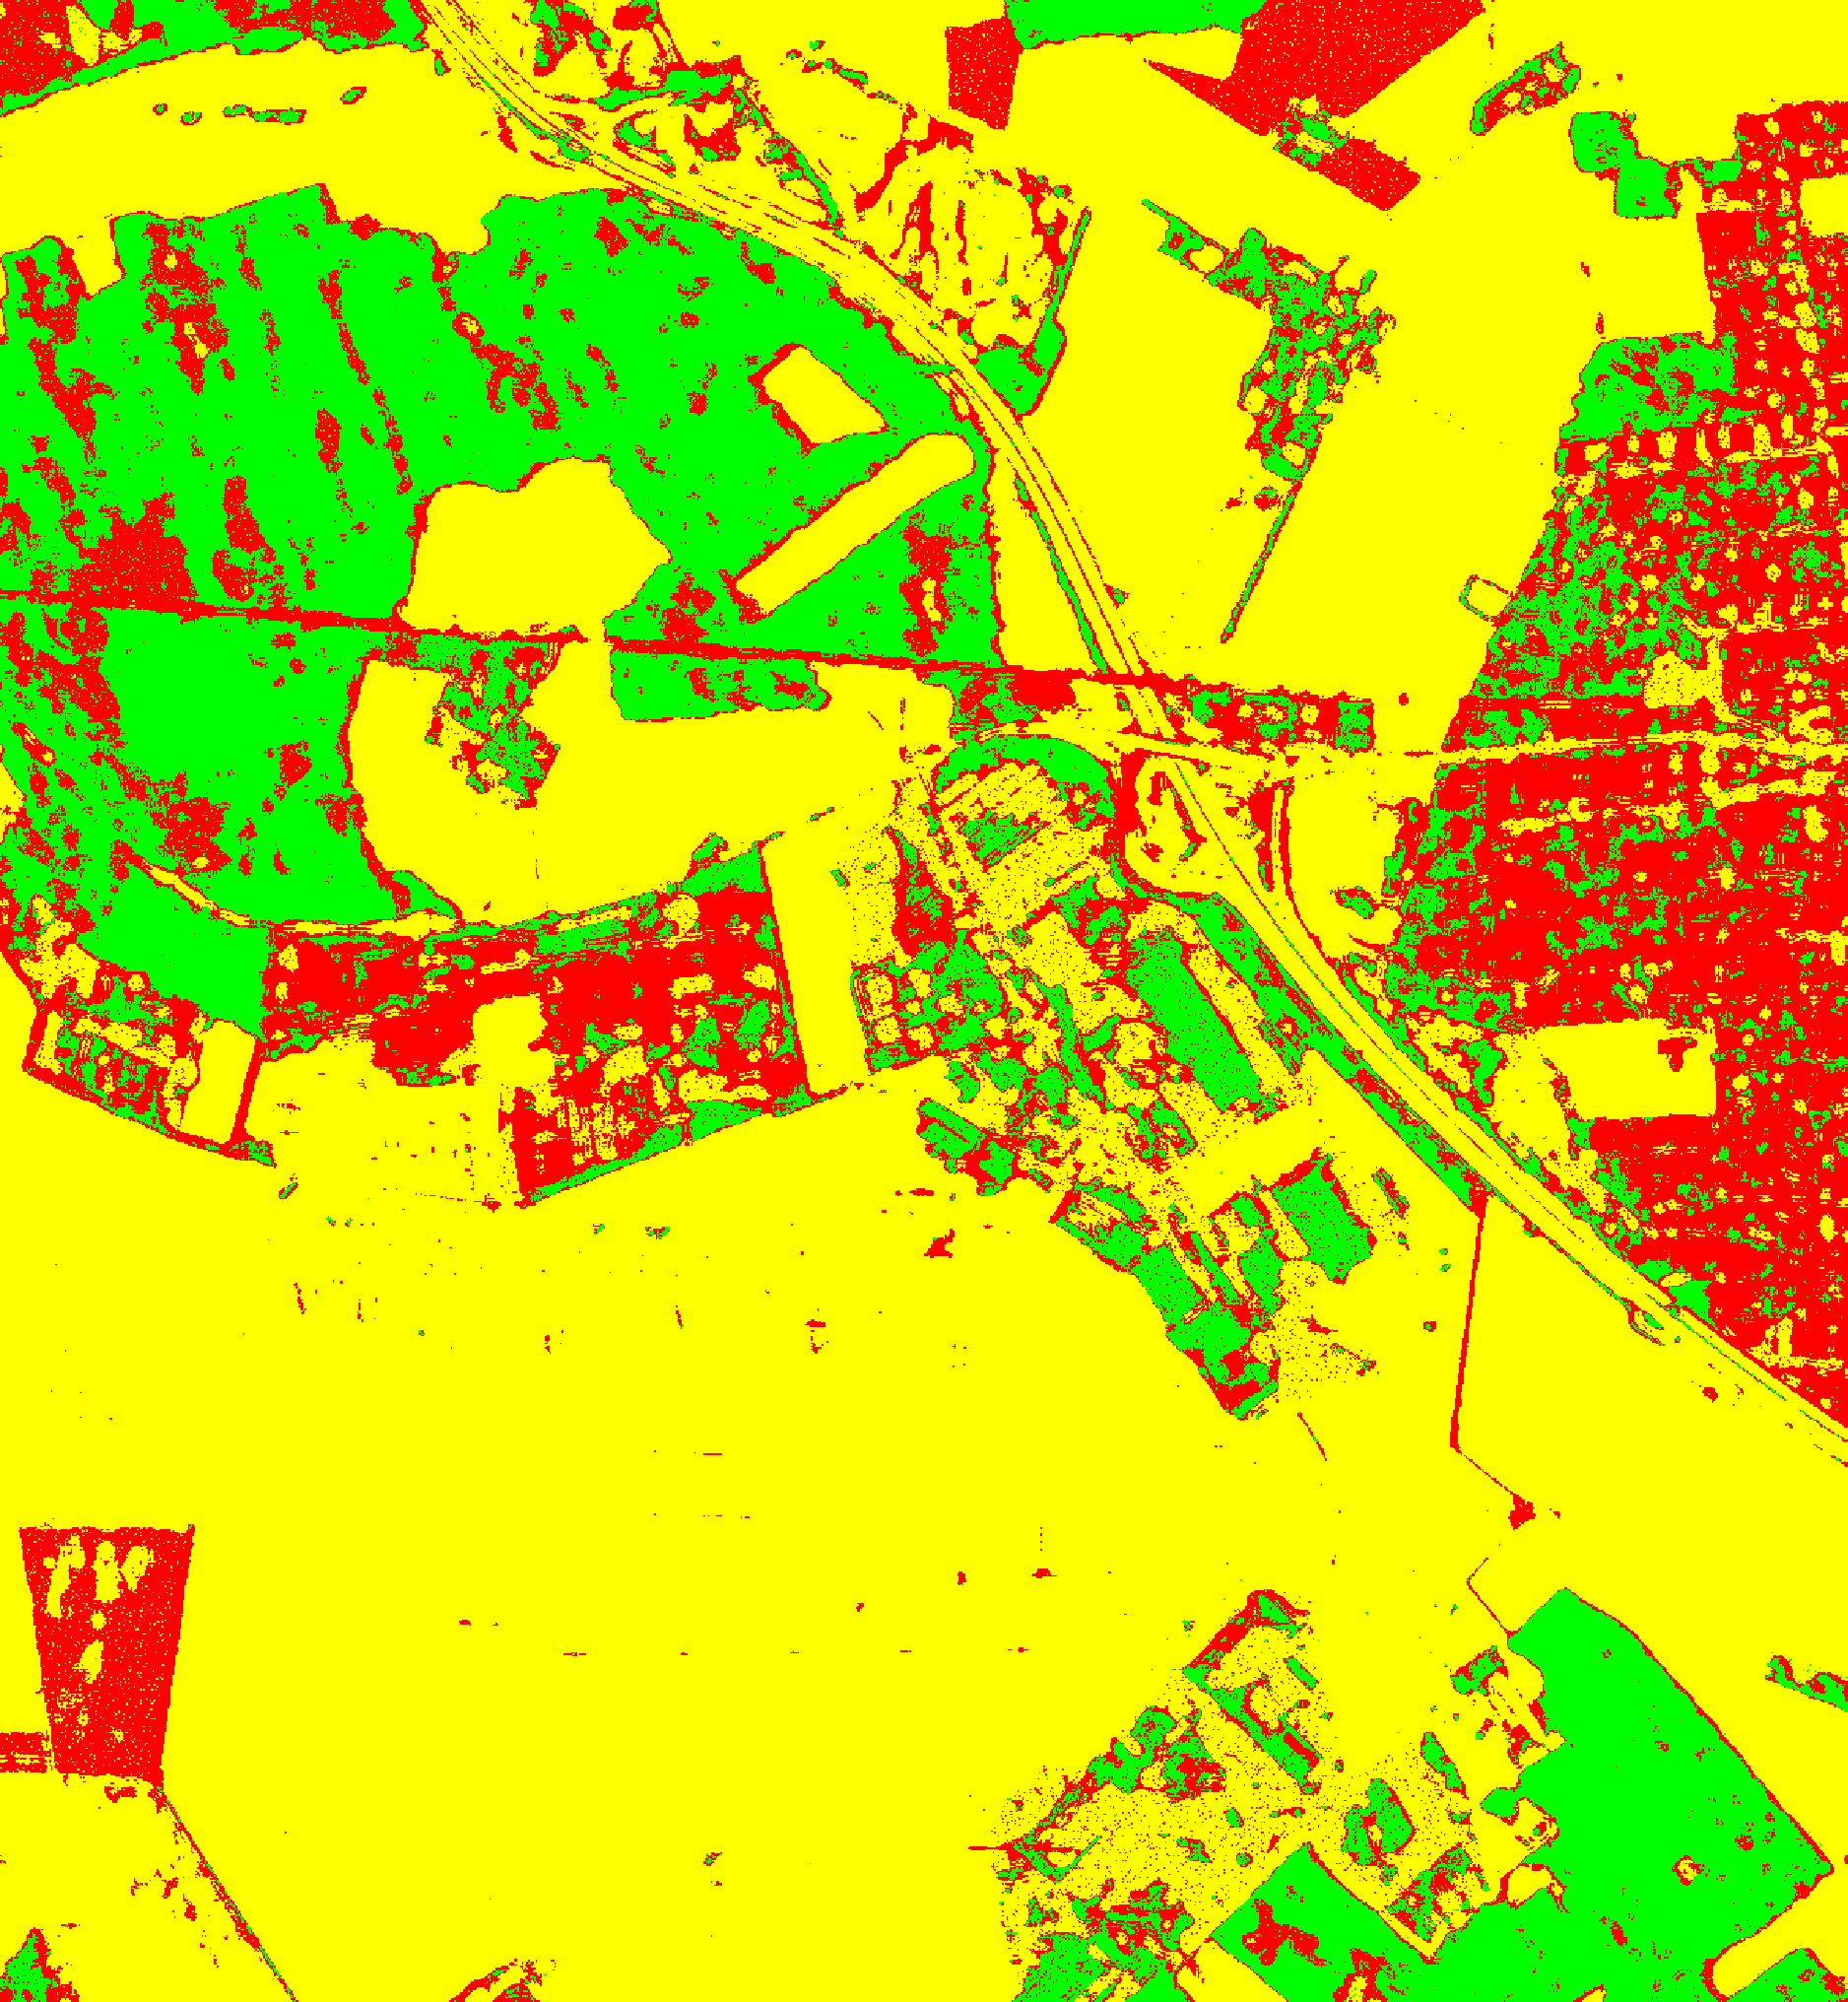
\includegraphics[width=4.04cm]{pic/chapter4/ober/Wishart-10.png}
  }
  \subfloat[]{
    \label{fig:ober_SVM}
    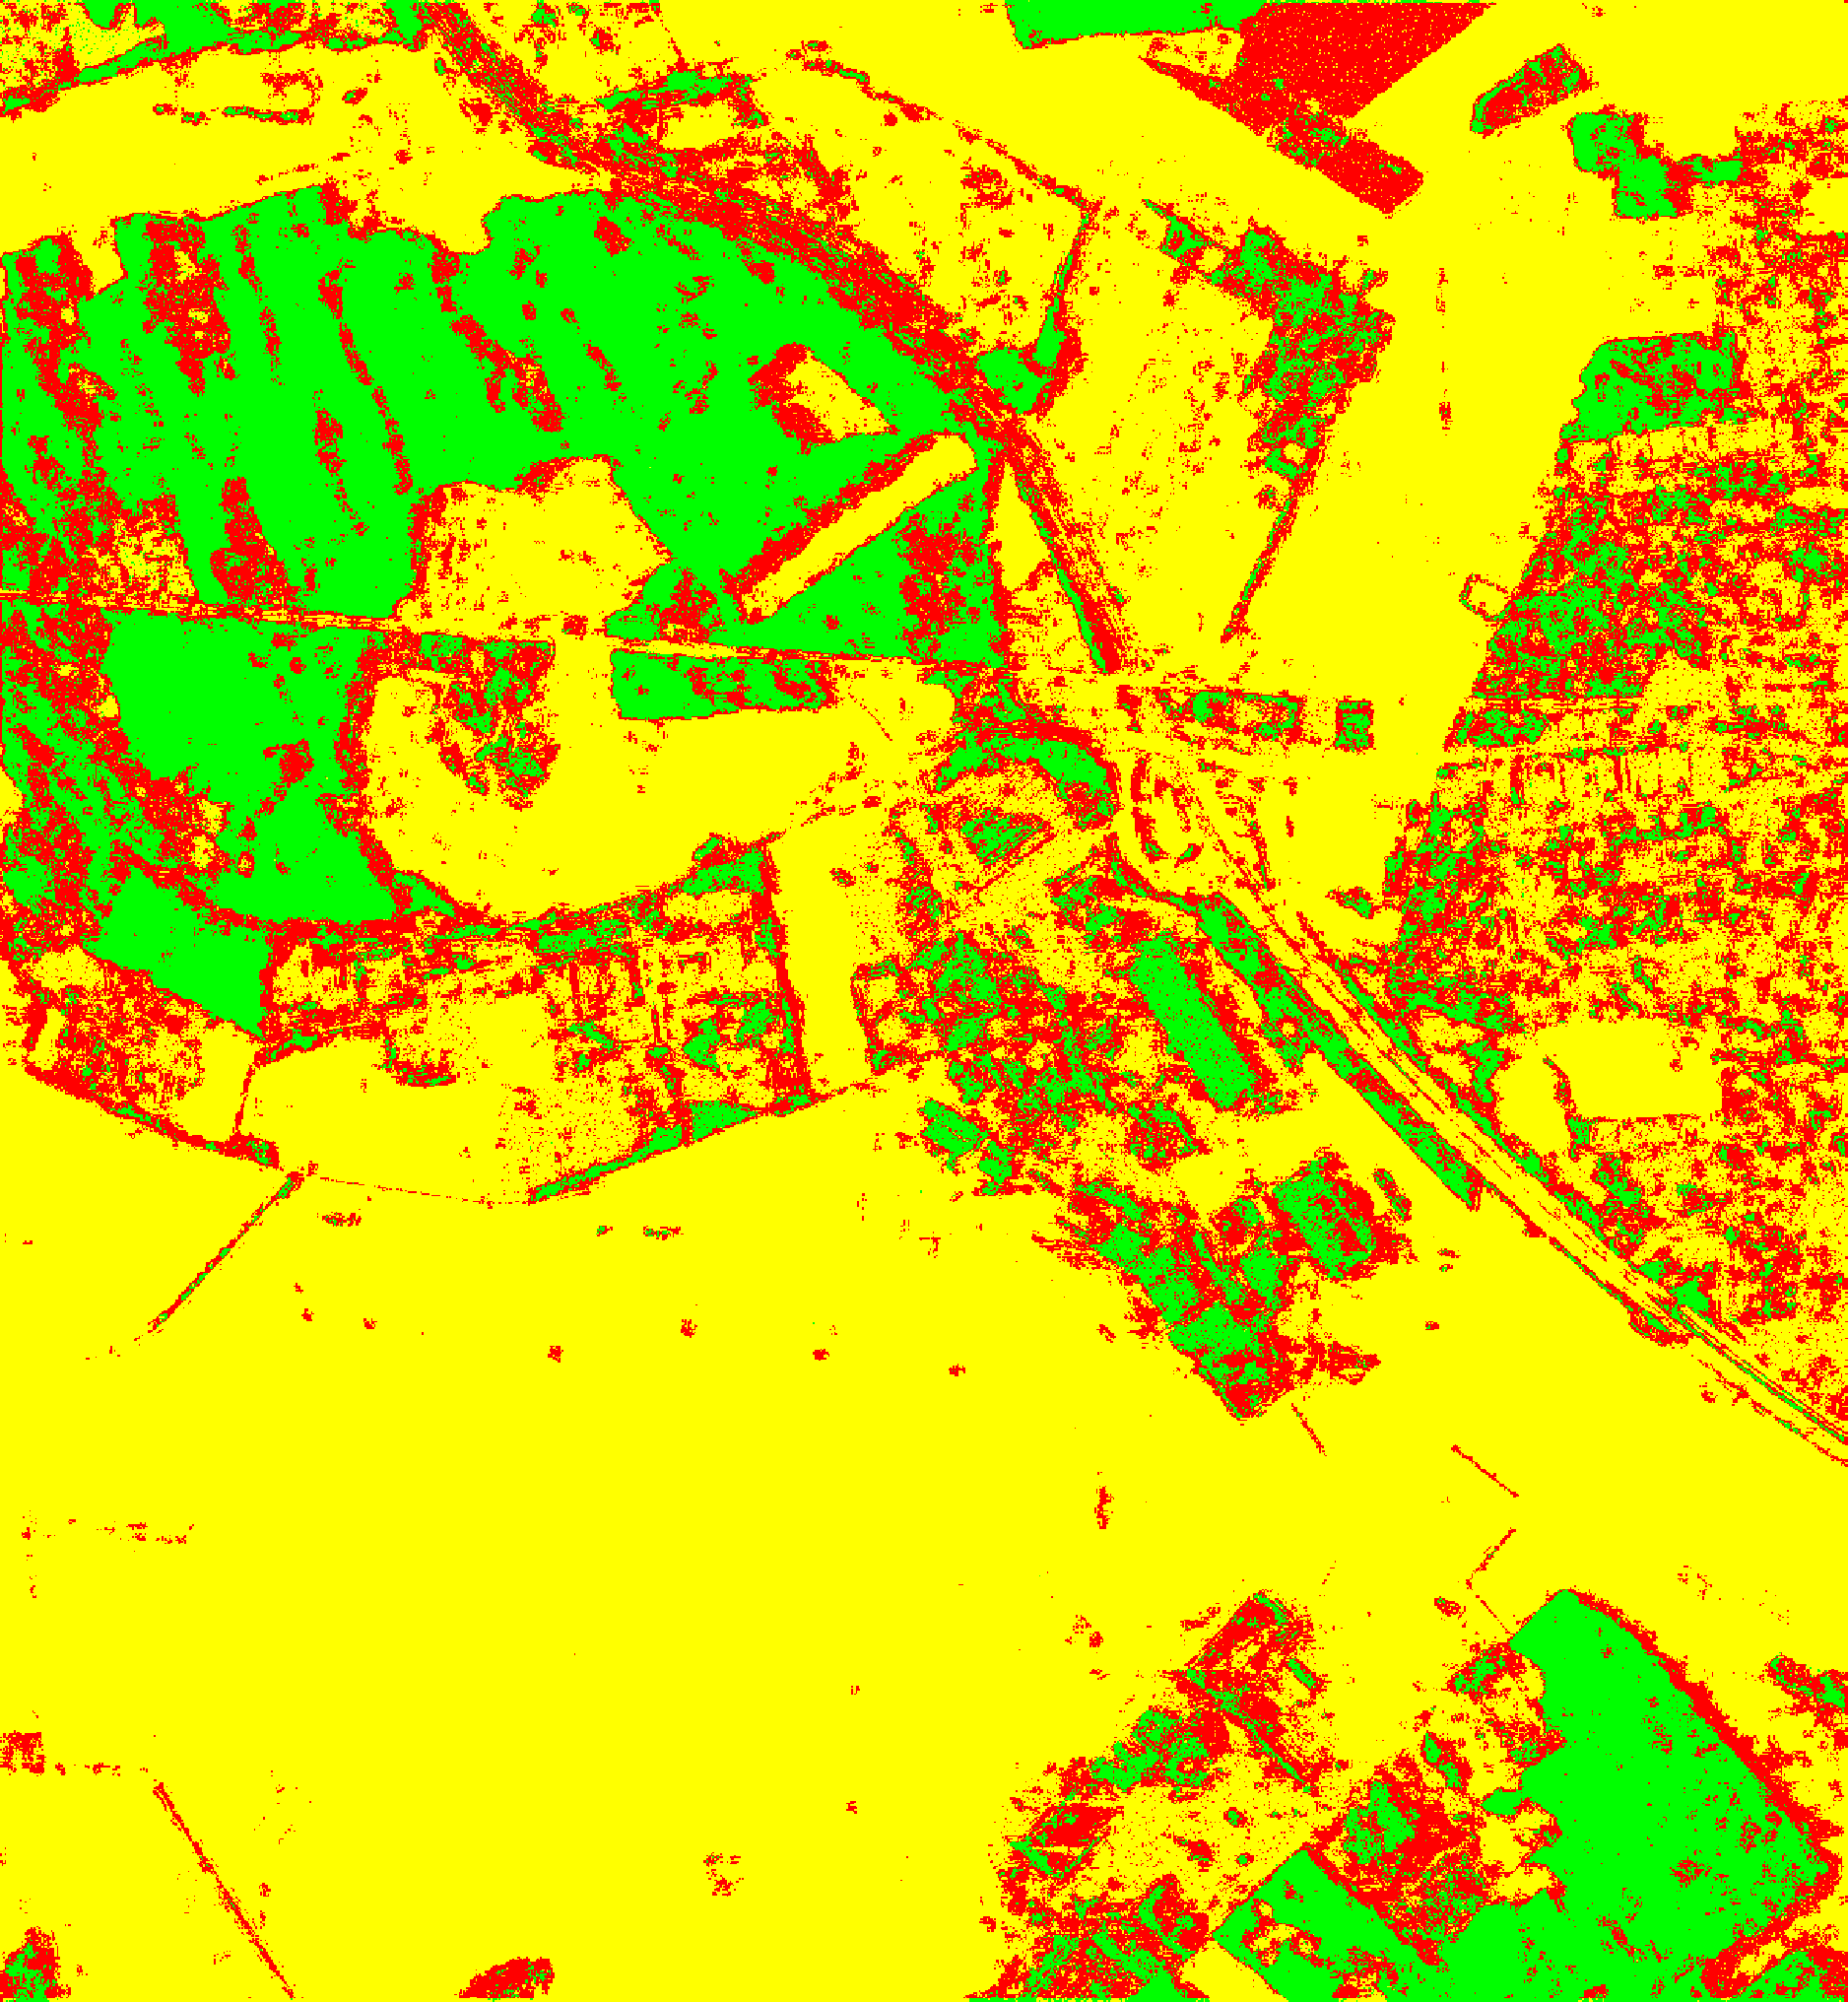
\includegraphics[width=4.04cm]{pic/chapter4/ober/SVM-10.png}
  }
  \subfloat[]{
    \label{fig:ober_CNN}
    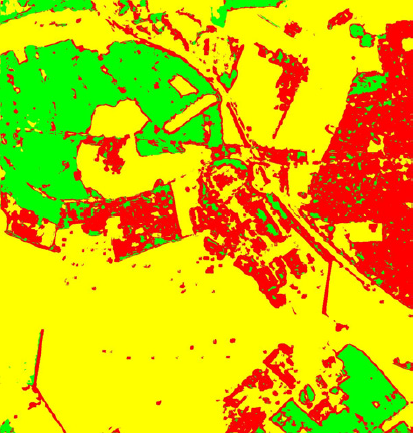
\includegraphics[width=4.04cm]{pic/chapter4/ober/CNN-10.png}
  }

  \subfloat[]{
    \label{fig:ober_RSL}
    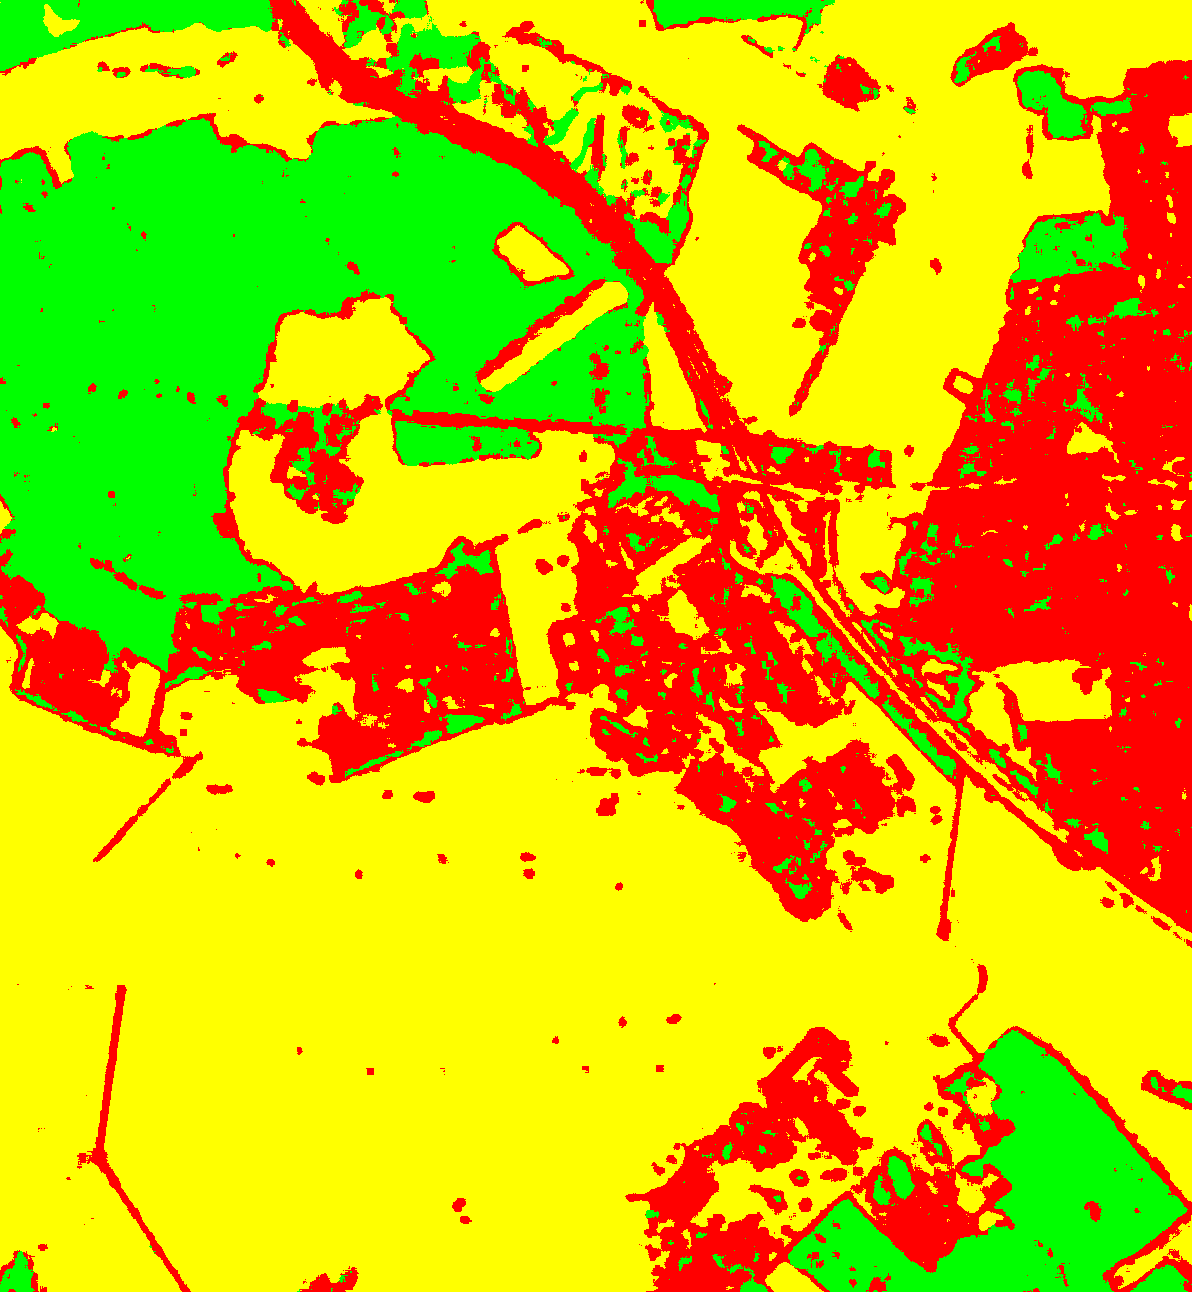
\includegraphics[width=4.04cm]{pic/chapter4/ober/RSL-10.png}
  }
  \subfloat[]{
    \label{fig:ober_BEL}
    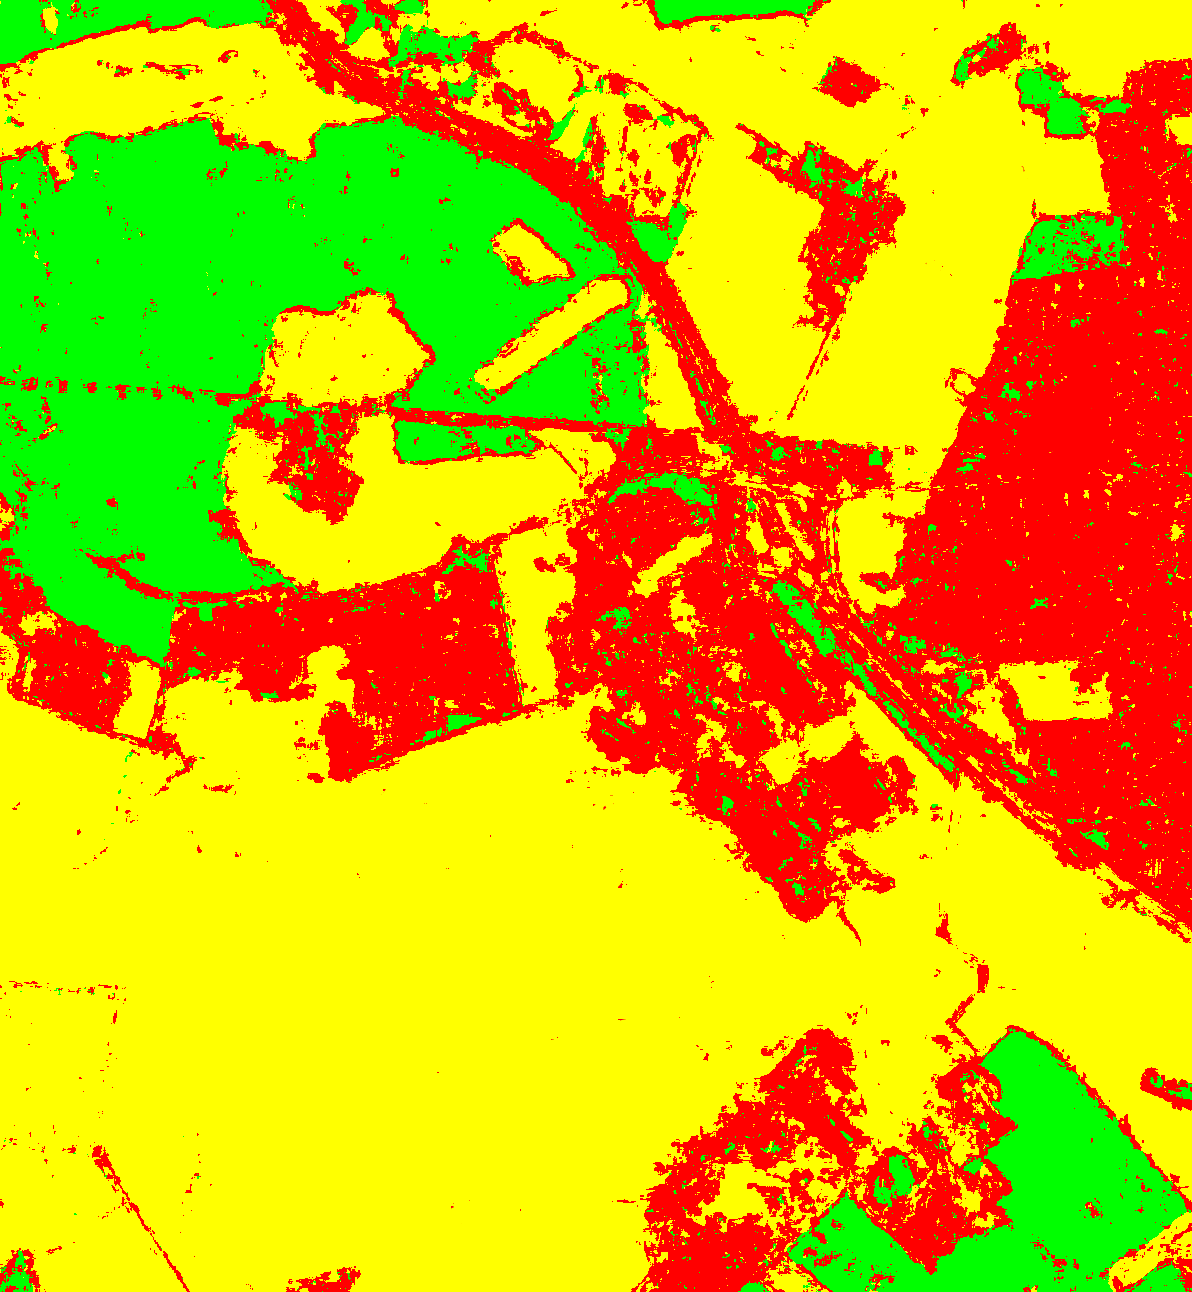
\includegraphics[width=4.04cm]{pic/chapter4/ober/BEL-10.png}
  }
  \subfloat[]{
    \label{fig:ober_BEL_DP}
    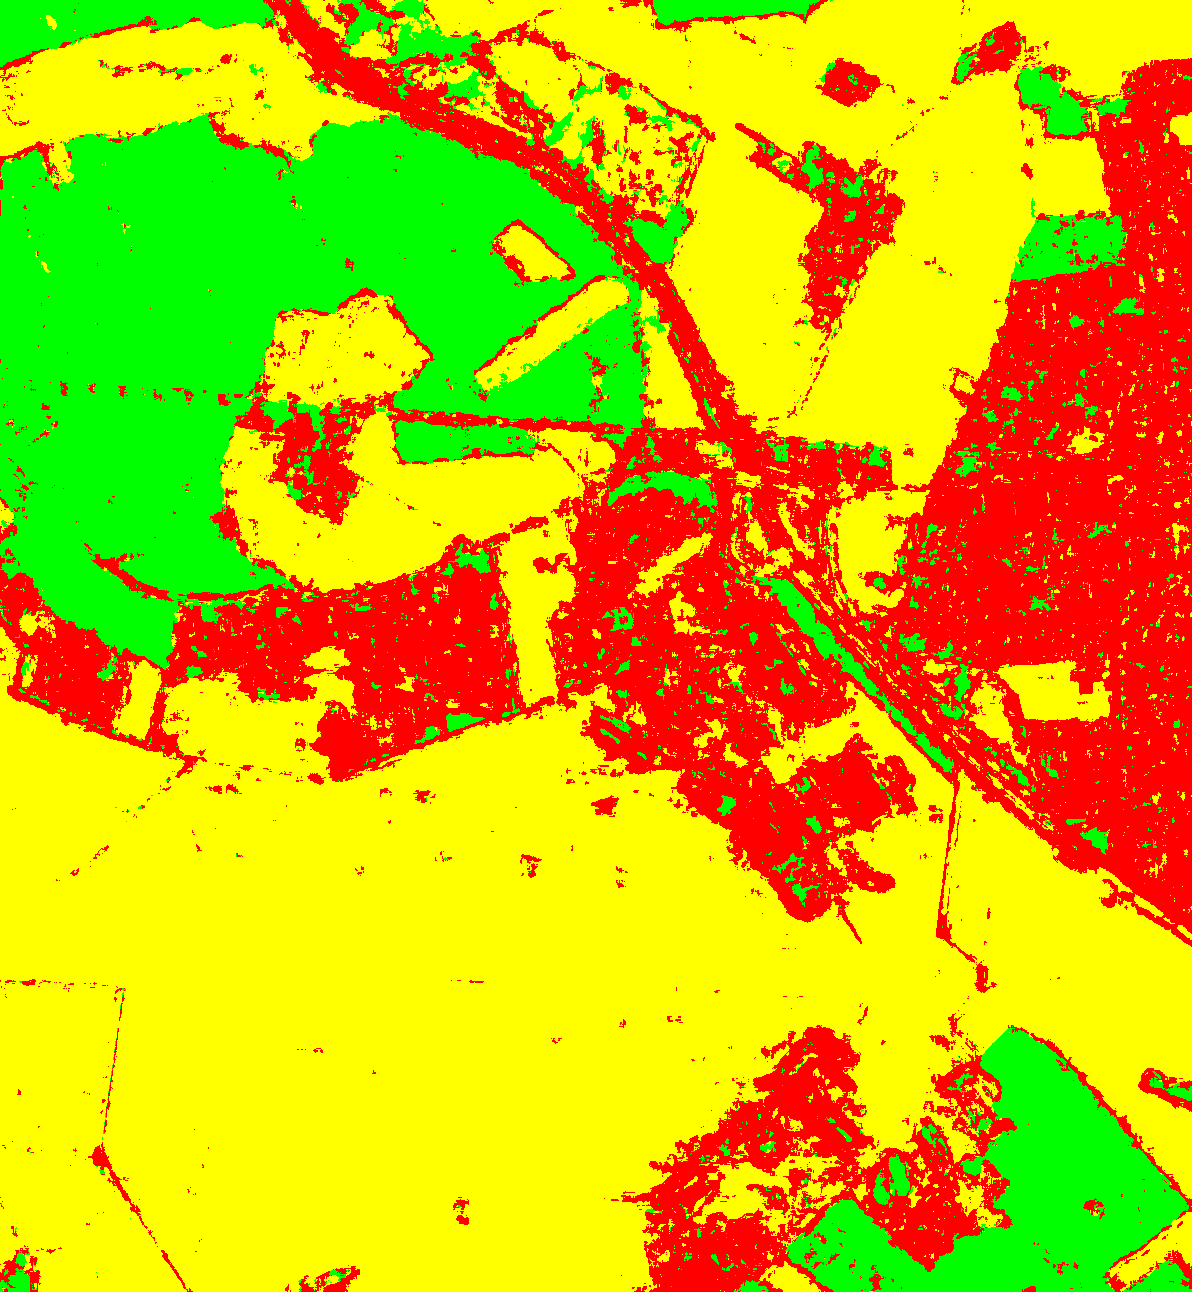
\includegraphics[width=4.04cm]{pic/chapter4/ober/BEL_DP-10.png}
  }

  \subfloat[]{
    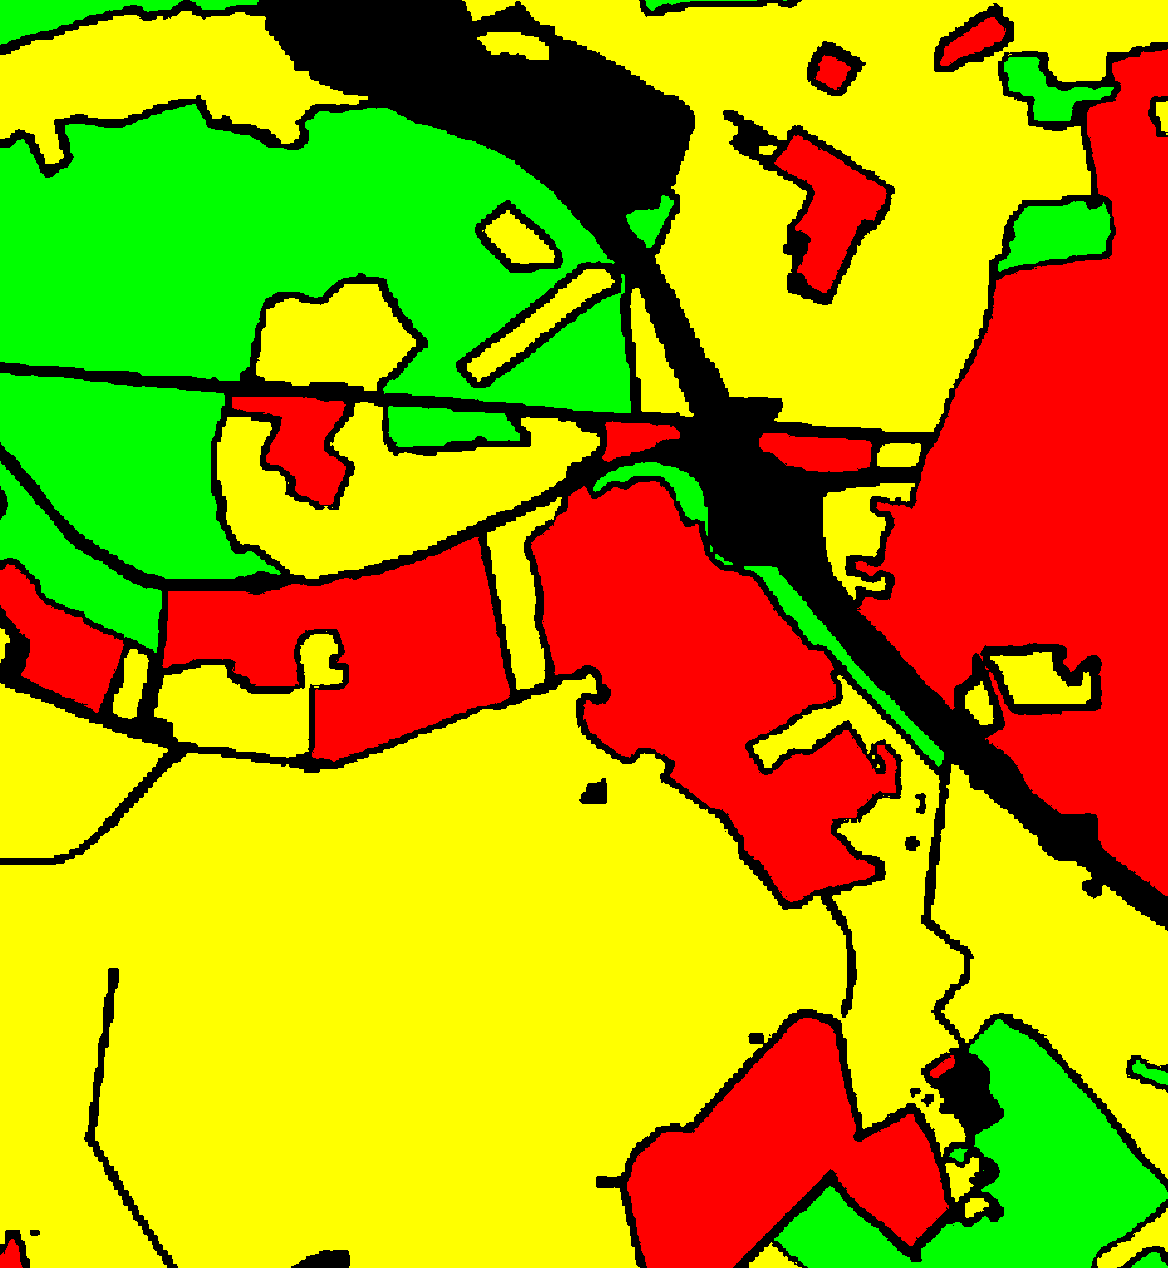
\includegraphics[width=4.04cm]{pic/chapter4/ober/gt.png}
  }
  \subfloat[]{
    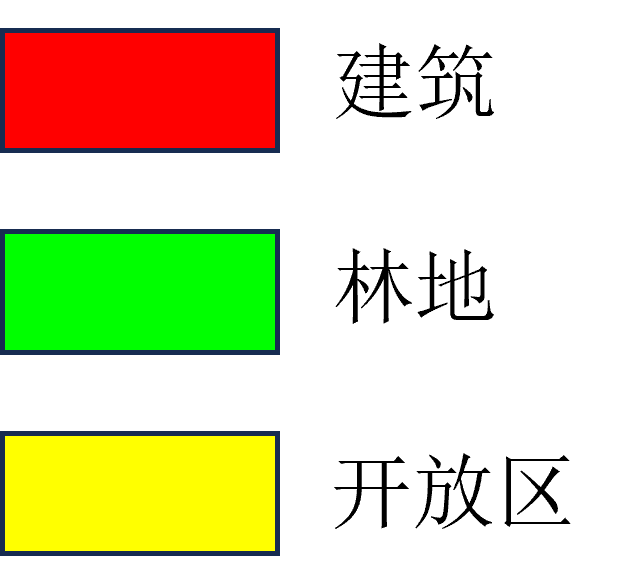
\includegraphics[width=2.04cm]{pic/chapter4/ober/label.png}
  }

  \caption{AIRSAR Flevoland地区数据对称标签噪声下分类可视化结果图。(a) SVM;(b)Wishart; (c) CNN; (d) RSL; (e) BEL; (f) BEL + DP; (g) 地面真值;(h) 颜色与类别对应关系}
  \label{fig:ober_res_random}
\end{figure}

表\ref{tab:ober_res_4}展示了不同实验方法在10\%比例对称标签噪声下的分类数值结果。其中,SVM与Wishart分类方法虽然在开放区域的分类准确率取得了不错的效果,分别为95.28\%和95.21\%,但是由于在建筑区域和林地区域分类效果均不理想,导致整体准确率、平均准确率、Kappa系数三相指标都较低,这是因为噪声标签信息对该两个分类方法的影响,学习到错误的分类规则。RSL方法在林地区域单向准确率取得了最高的分类准确率为95.16\%,相比于本章方法提高了3.94\%,这可能是因为林地区域散射特性差异大,极化信息提取器在该区域的提升性能不足,同时该区域训练样本充足,直接丢弃所有的可能为噪声的样本并未丢失关键的数据分布特征。RSL+DP方法在综合指标方面均取得了最高值,分别为94.55\%、93.52\%和90.66\%,相比于其他方法分别提升了4.76\%、5.6\%和1.23\%。综上所述,本章方法在噪声标签条件下的数据集中具有更优越的分类性能。

\begin{table}[ht!]
  \caption{ESAR Oberpfaffenhofen地区数据对称标签噪声下分类数值结果(\%)}
  \label{tab:ober_res_4}
  \begin{tabular}{cccccccc}
    \toprule[1.5bp]
    序号                        & 类别    & SVM   & Wishart & CNN   & RSL            & BEL            & BEL+DP         \\
    \midrule[0.75bp]
    1                         & 建筑    & 75.19 & 61.35   & 81.25 & 75.32          & 89.98          & \textbf{92.35} \\
    2                         & 林地    & 76.54 & 74.58   & 80.24 & \textbf{95.16} & 91.59          & 91.82          \\
    3                         & 开放区域  & 95.28 & 95.21   & 85.82 & 93.28          & 93.39          & \textbf{96.38} \\
    \midrule[0.75bp]
    \multicolumn{2}{c}{OA}    & 79.07 & 83.05 & 83.67   & 89.79 & 92.56          & \textbf{94.55}                  \\
    \multicolumn{2}{c}{AA}    & 82.33 & 77.04 & 82.44   & 87.92 & 91.65          & \textbf{93.52}                  \\
    \multicolumn{2}{c}{Kappa} & 77.25 & 70.45 & 79.14   & 89.43 & 89.68          & \textbf{90.66}                  \\
    \bottomrule[0.75bp]
  \end{tabular}
\end{table}

\subsubsection{非对称标签实验}
图\ref{fig:ober_noise_random}展示了10\%噪声比例下非对称标签噪声的噪声转移矩阵,每个类别正确标记的概率为90\%,10\%的标签噪声随机映射到另外的一个类别中。
\begin{figure}[ht!]
  \centering
  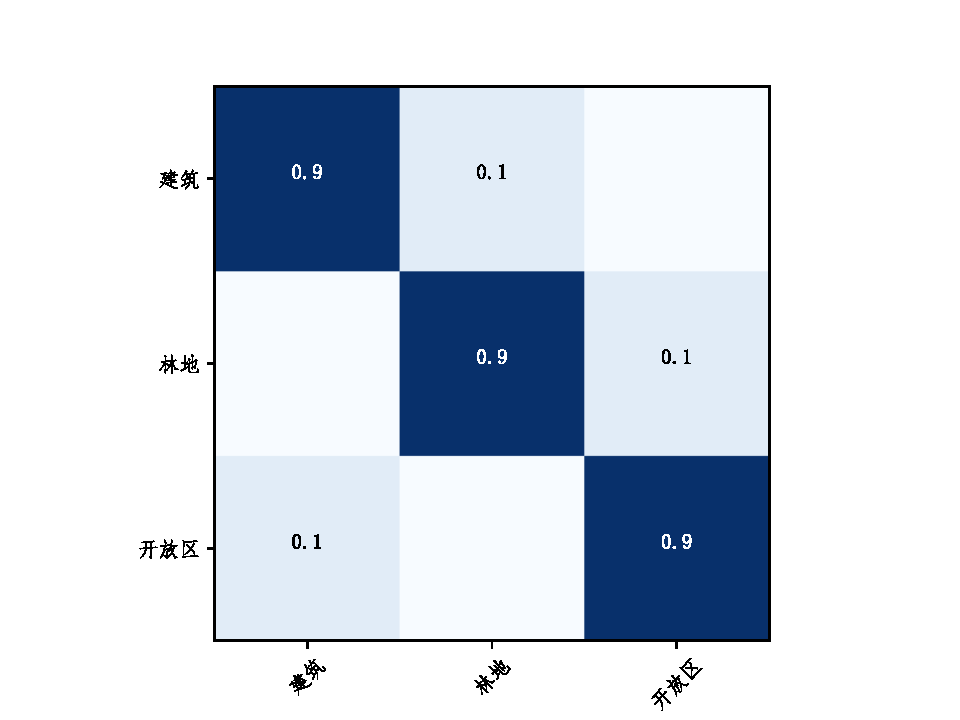
\includegraphics[width=10.04cm]{pic/chapter4/ober/noise_random.pdf}
  \caption{ESAR Oberpfaffenhofen数据10\%非对称噪声转移矩阵}
  \label{fig:ober_noise_random}
\end{figure}

图\ref{fig:fle_res_random}展示了10\%非对称标签噪声下不同分类方法的分类结果。图\ref{fig:ober_Wishart_random}与图\ref{fig:ober_SVM_random}展示的Wishart与SVM的分类结果,可以在林地、建筑区域都存在较多的错误区域,分类效果差。图\ref{fig:ober_CNN_random}为交叉熵损失下的CNN分类结果,可以看到受到标签噪声影响,开放区域错分为建筑、建筑区域错分为林地的情况存在较多。图\ref{fig:ober_RSL_random}为RSL方法的分类结果。。。。图\ref{fig:ober_BEL_random}与图\ref{fig:ober_BEL_DP_random}为BEL与BEL+DP方法的分类结果,可以看出在建筑物区域和林地区域的错分情况减少,分类结果更加平滑。因此,证明了本章方法的有效性与优越性。
\begin{figure}[ht!]
  \subfloat[]{
    \label{fig:ober_Wishart_random}
    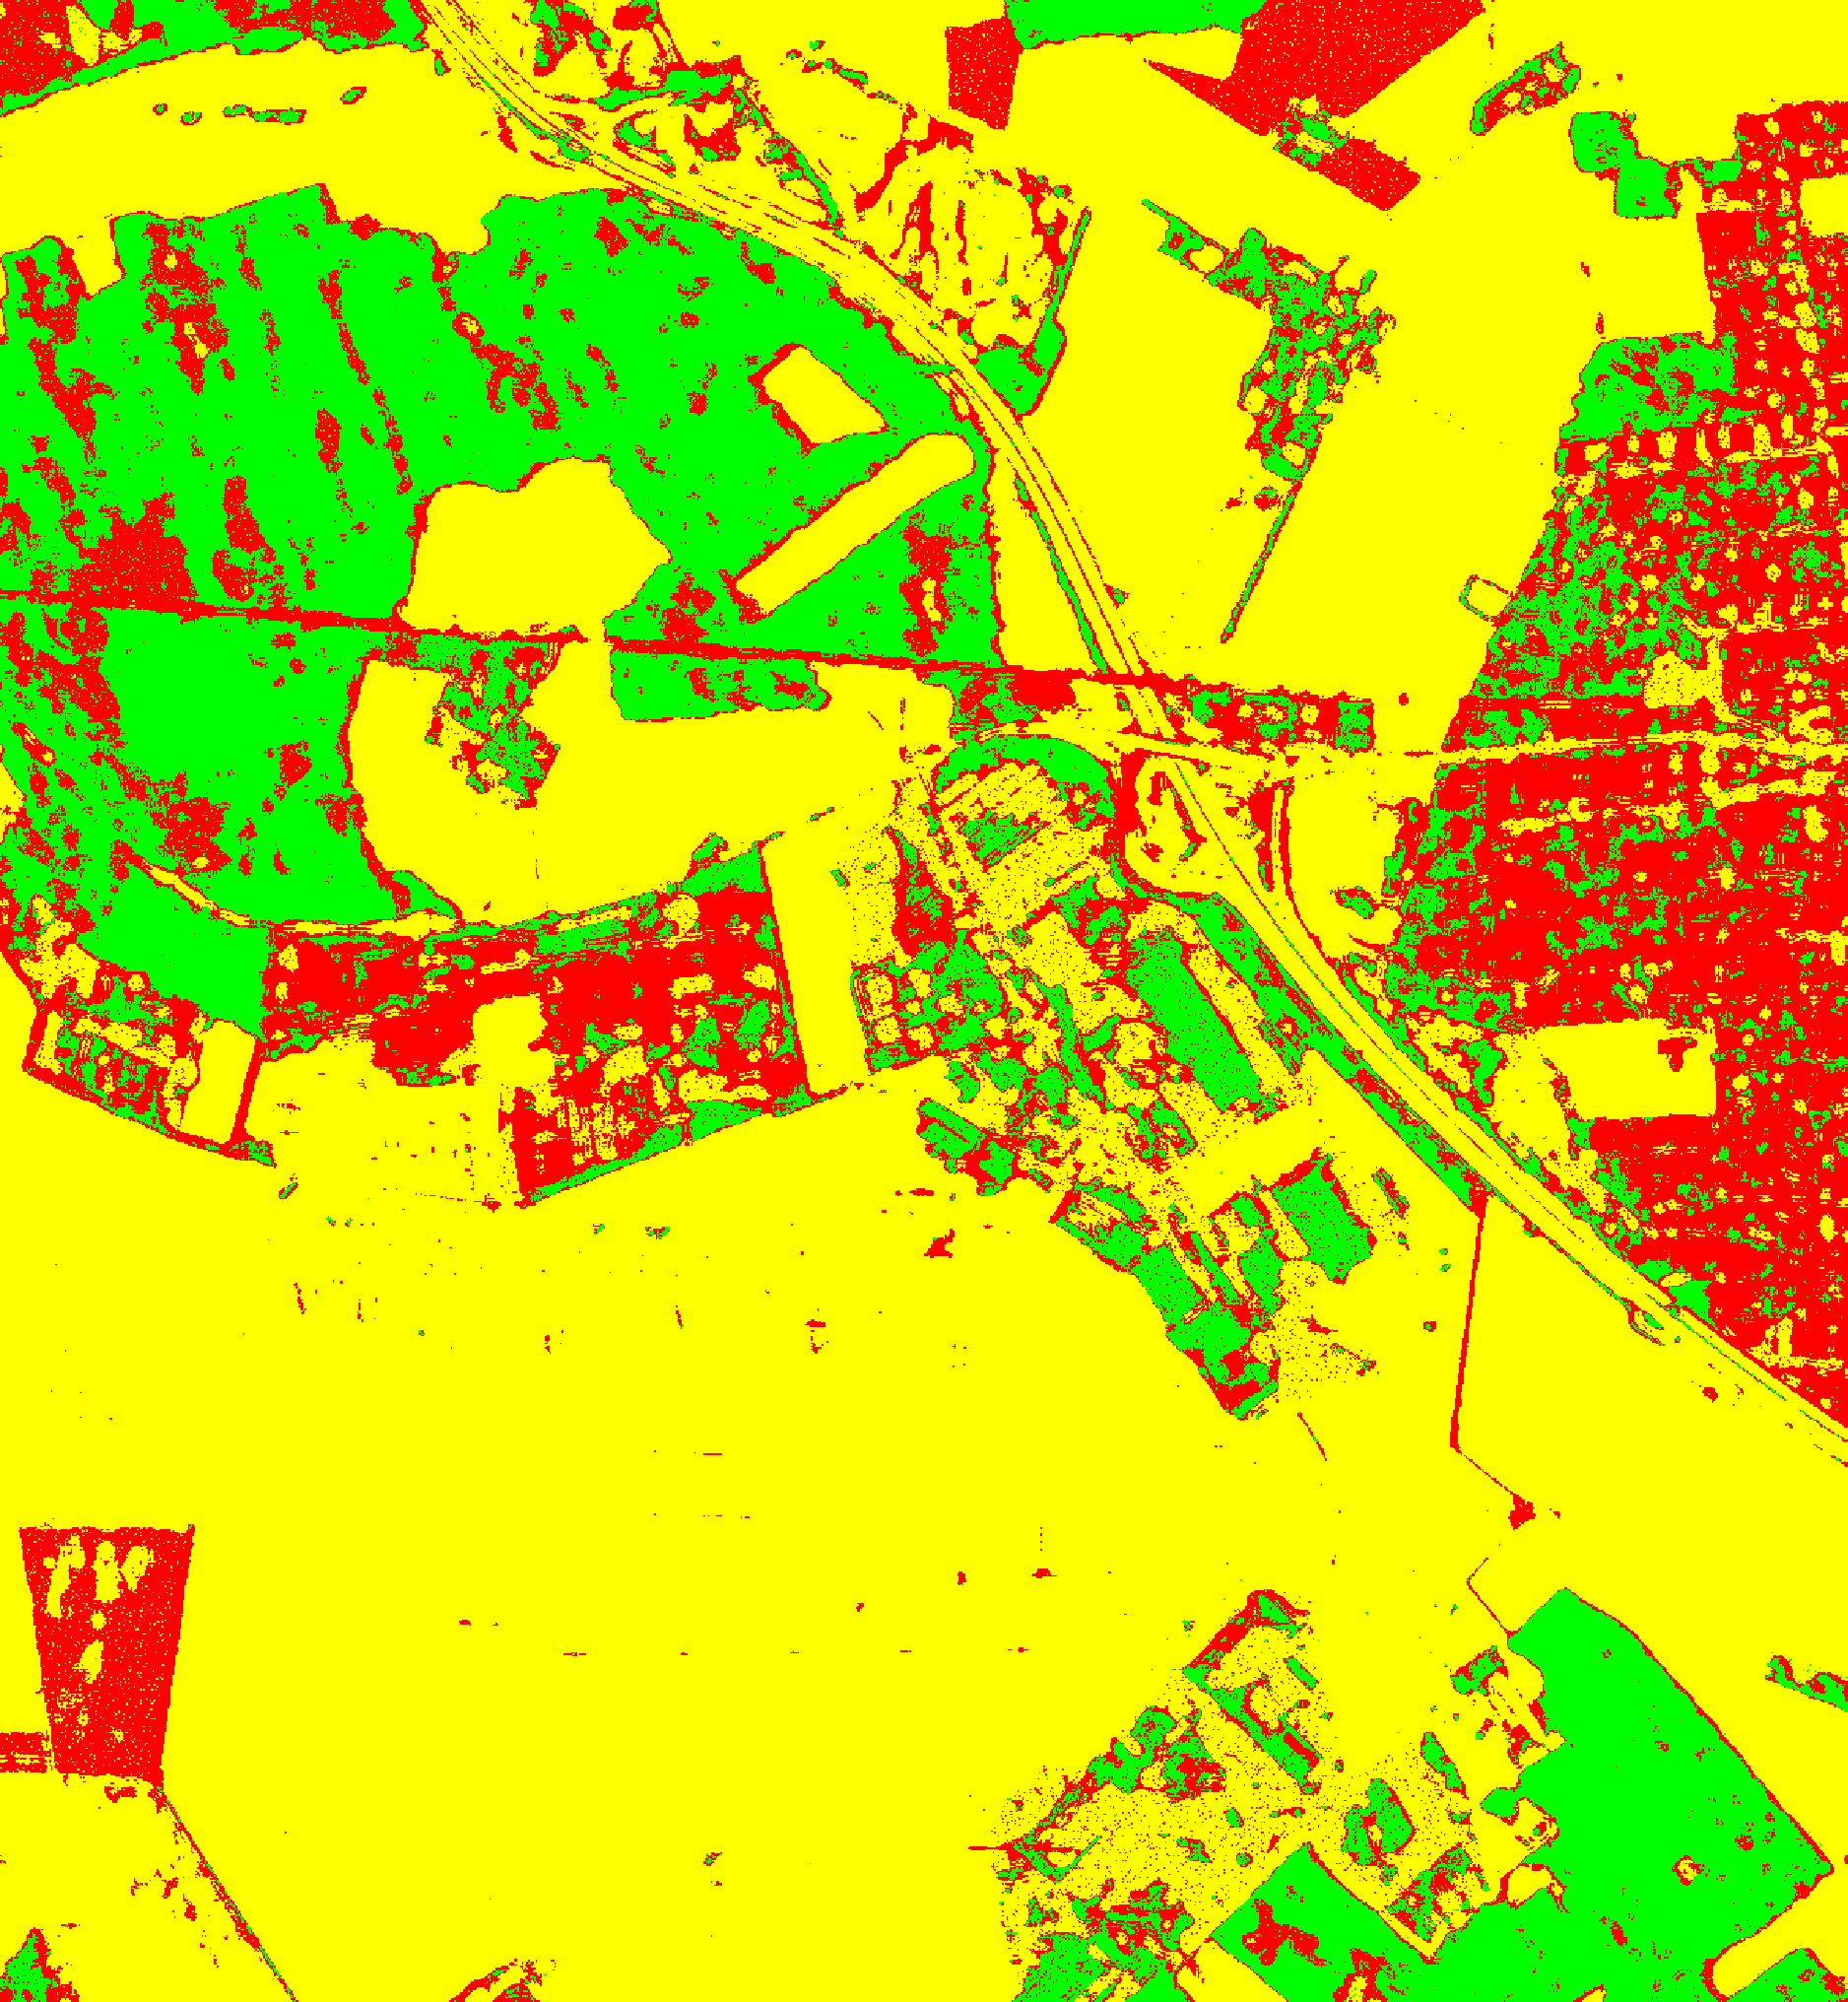
\includegraphics[width=4.04cm]{pic/chapter4/ober/Wishart-10.png}
  }
  \subfloat[]{
    \label{fig:ober_SVM_random}
    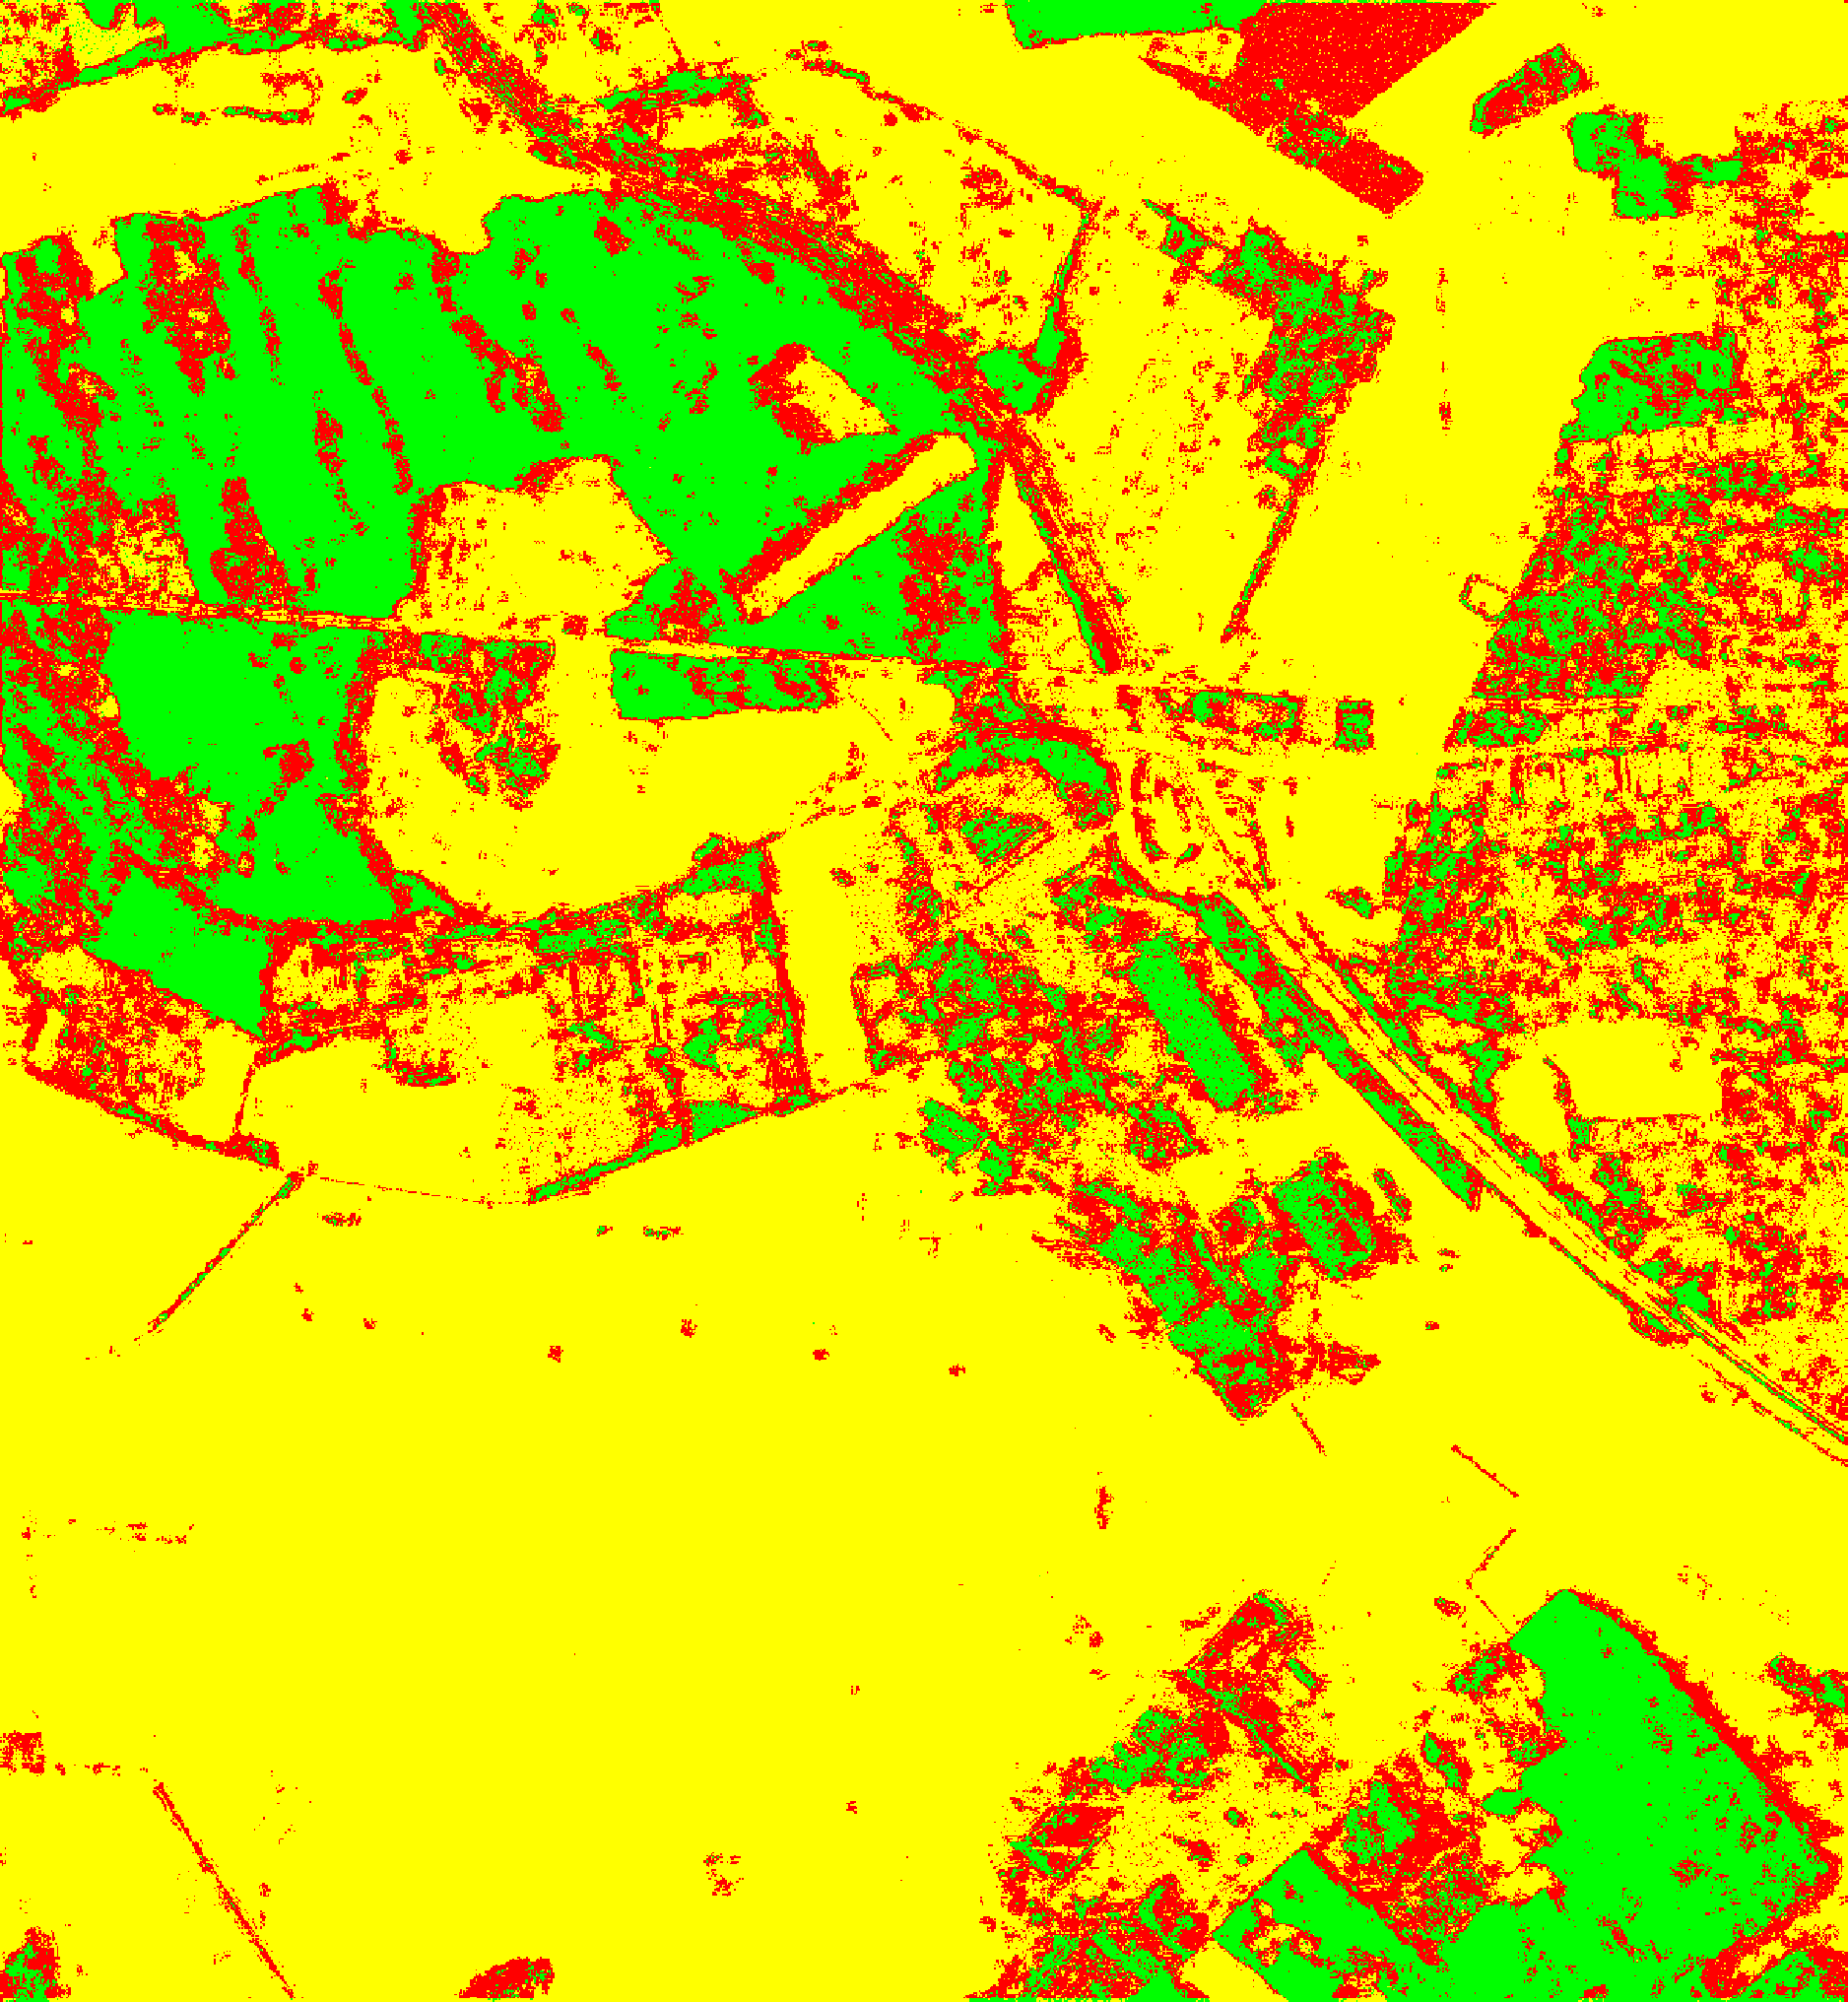
\includegraphics[width=4.04cm]{pic/chapter4/ober/SVM-10.png}
  }
  \subfloat[]{
    \label{fig:ober_CNN_random}
    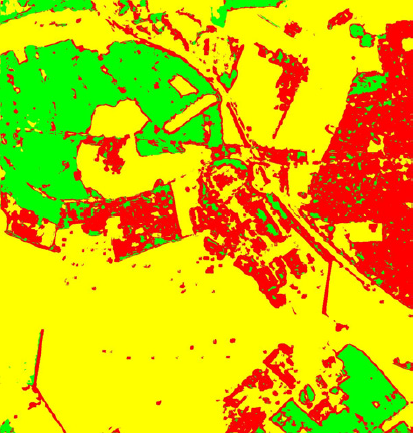
\includegraphics[width=4.04cm]{pic/chapter4/ober/CNN-10-random.png}
  }

  \subfloat[]{
    \label{fig:ober_RSL_random}
    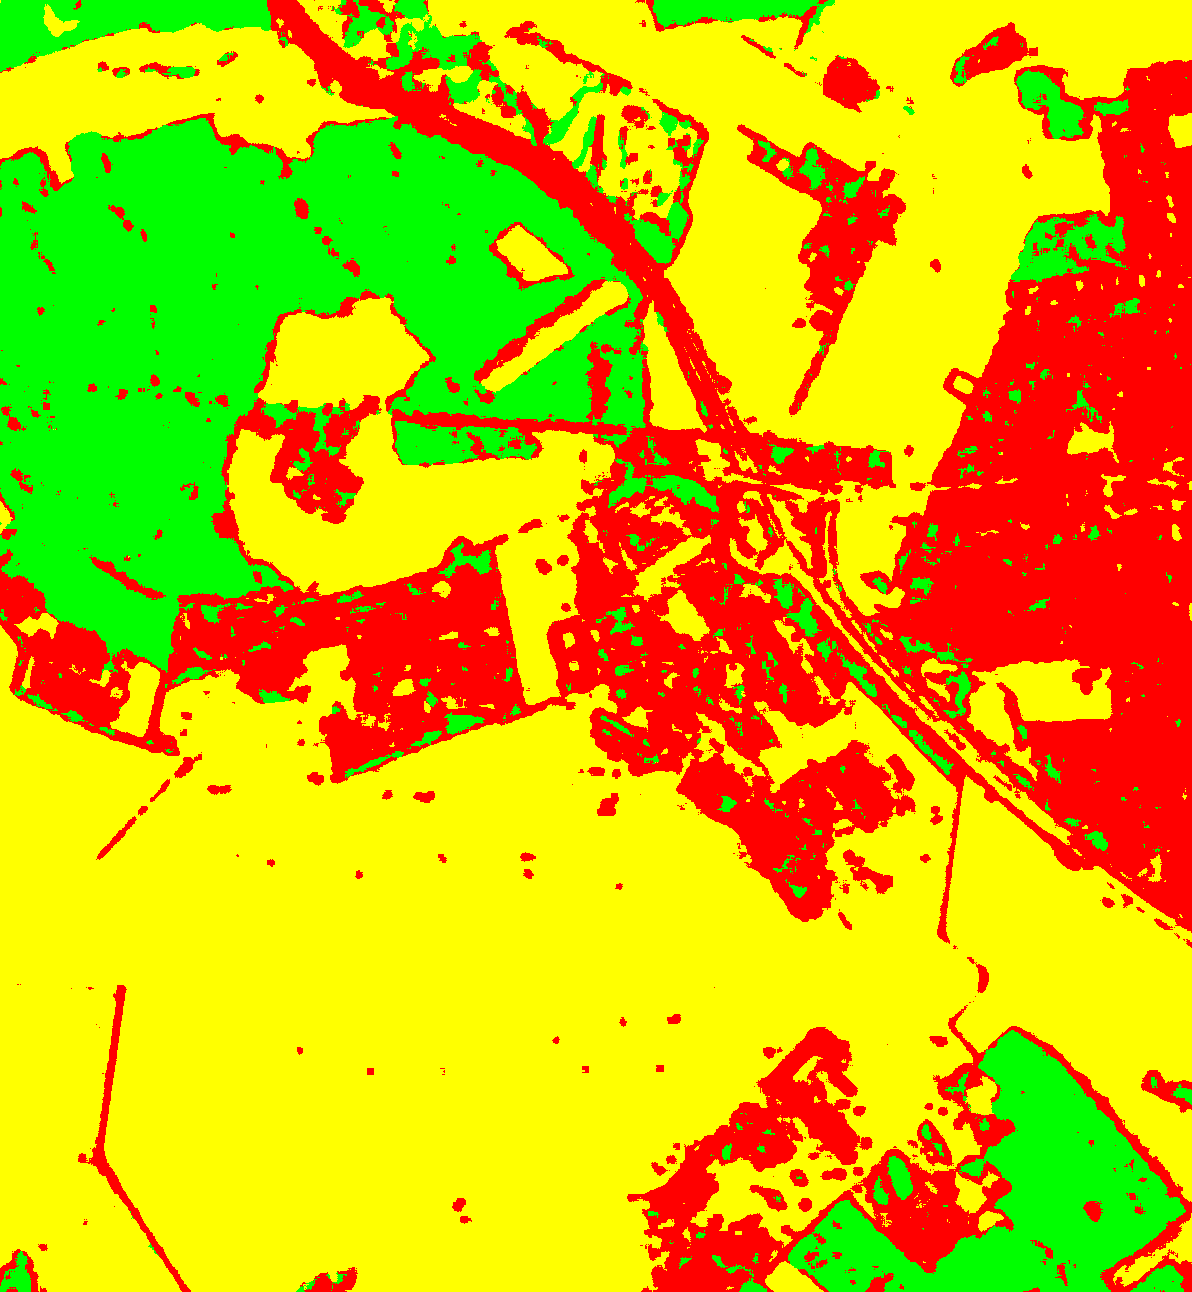
\includegraphics[width=4.04cm]{pic/chapter4/ober/RSL-10-random.png}
  }
  \subfloat[]{
    \label{fig:ober_BEL_random}
    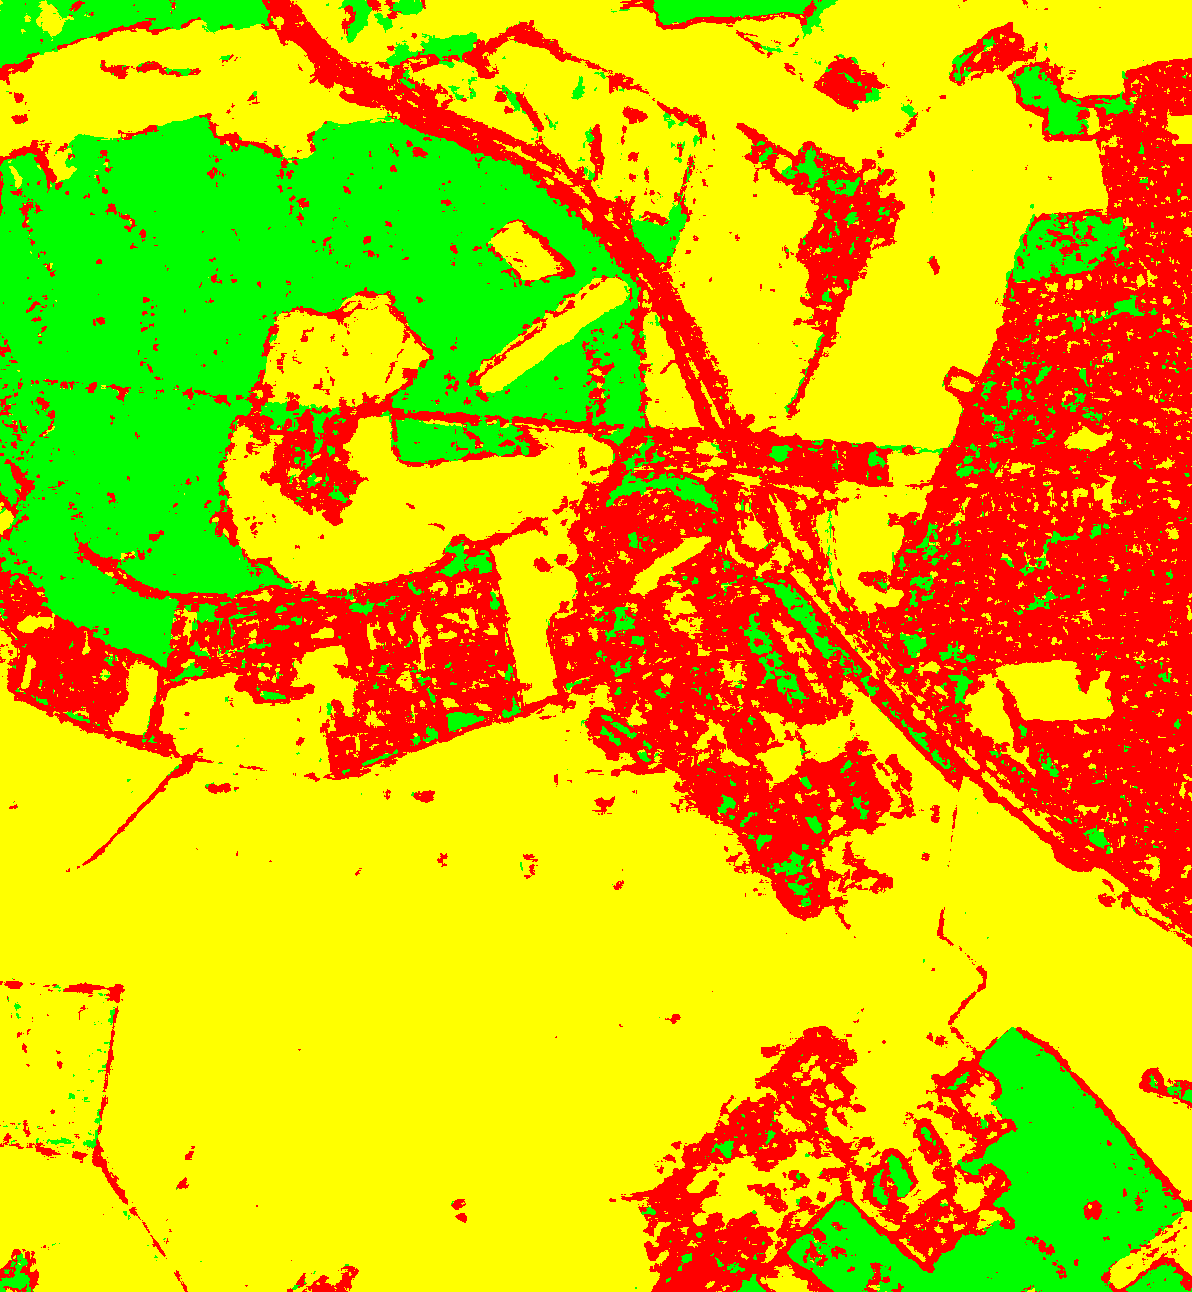
\includegraphics[width=4.04cm]{pic/chapter4/ober/BEL-10-random.png}
  }
  \subfloat[]{
    \label{fig:ober_BEL_DP_random}
    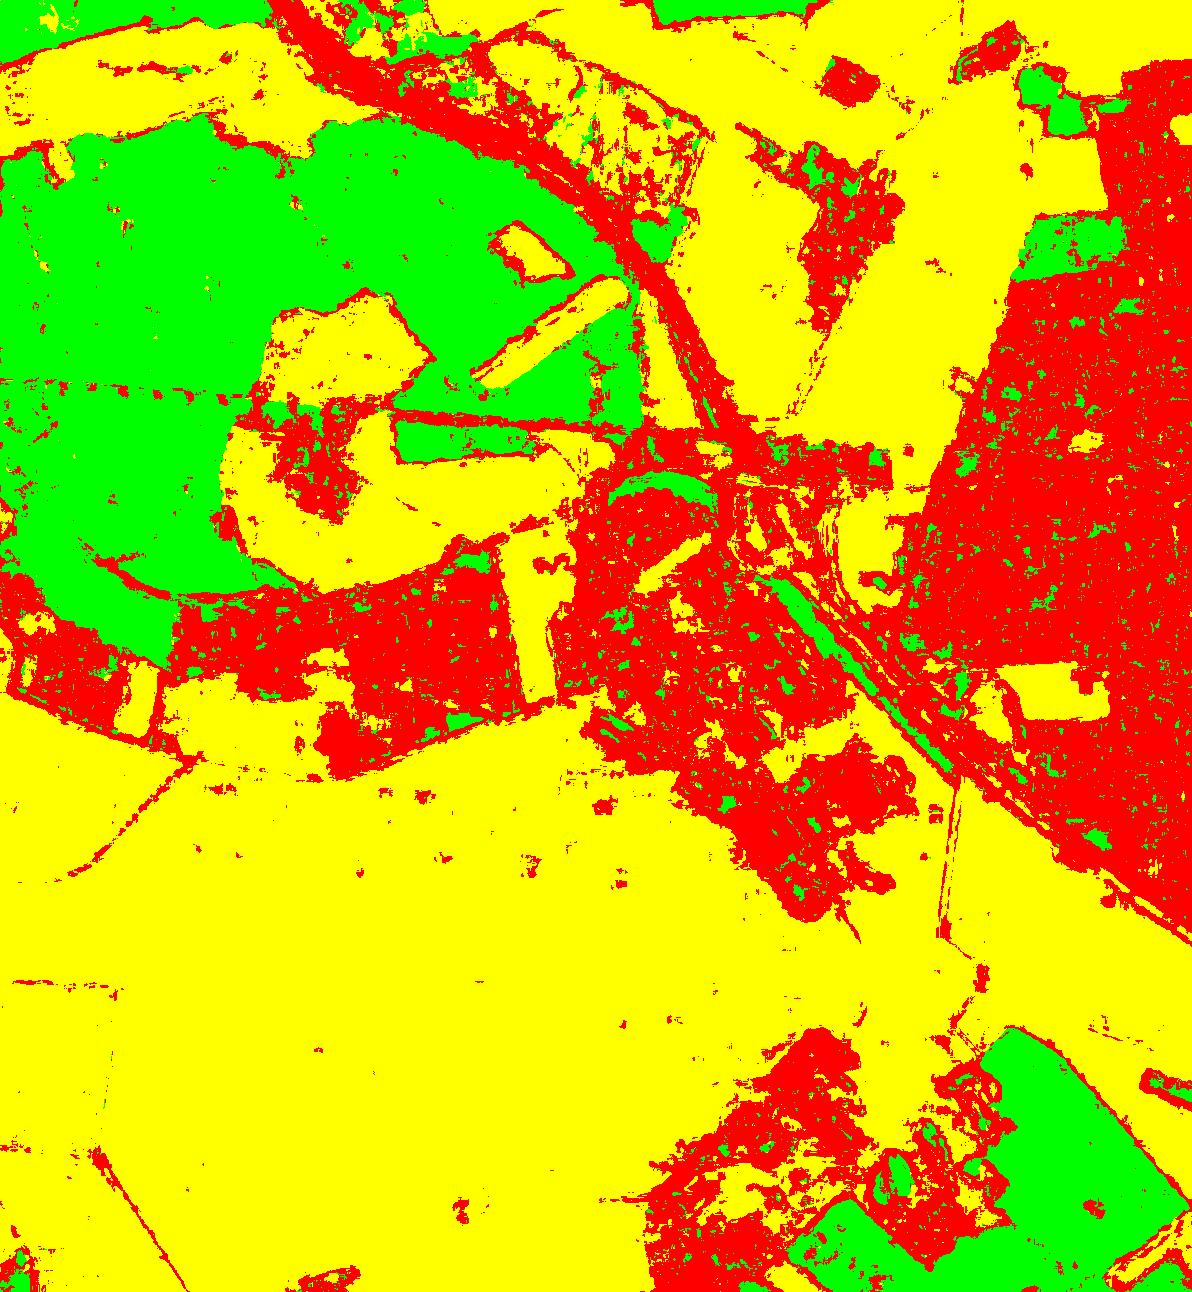
\includegraphics[width=4.04cm]{pic/chapter4/ober/BEL_DP-random.png}
  }

  \subfloat[]{
    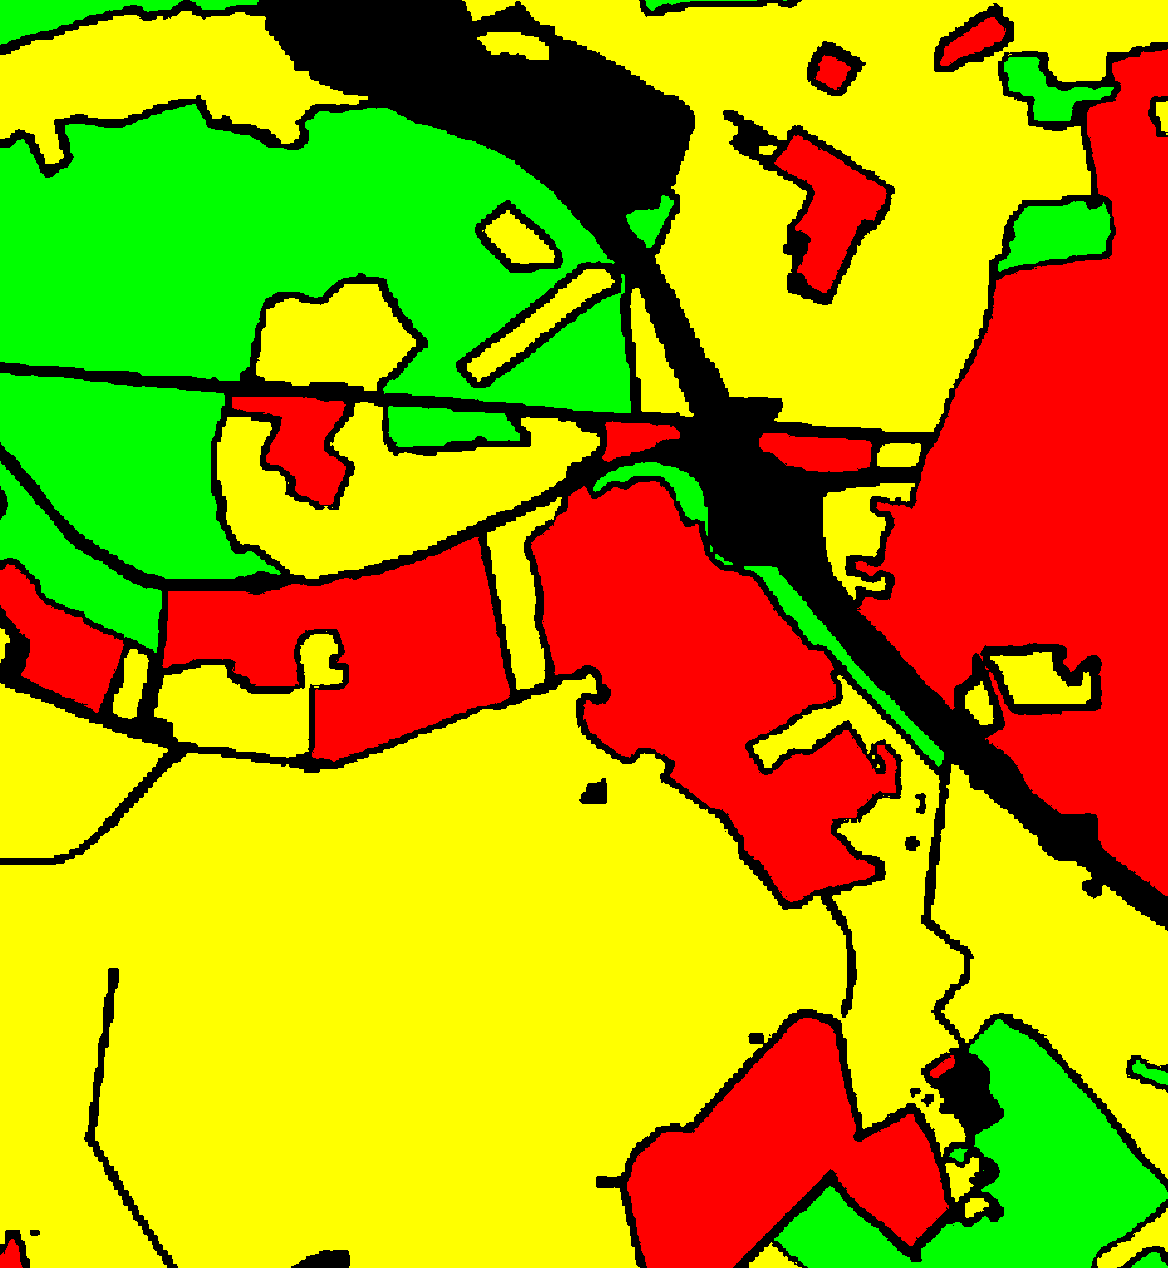
\includegraphics[width=4.04cm]{pic/chapter4/ober/gt.png}
  }
  \subfloat[]{
    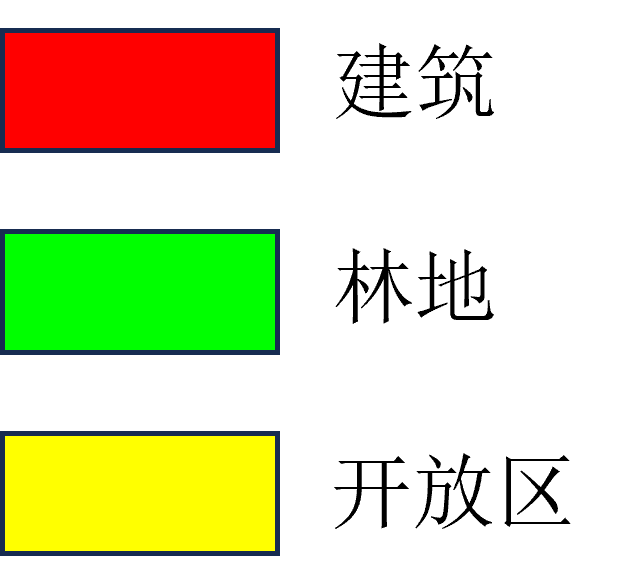
\includegraphics[width=2.04cm]{pic/chapter4/ober/label.png}
  }

  \caption{AIRSAR Flevoland地区数据非对称标签噪声下分类可视化结果图。(a) SVM;(b)Wishart; (c) CNN; (d) RSL; (e) BEL; (f) BEL + DP; (g) 地面真值;(h) 颜色与类别对应关系}
  \label{fig:fle_res_random}
\end{figure}

表\ref{tab:ober_res_random}展示了非对称标签噪声下的分类数值结果。SVM、Wishart以及CNN方法在建筑区域的分类准确率较低,导致总体准确率较低,分别为76.58\%,80.32\%,82.49\%,这是因为这三个方法均没有筛选错误样本的能力,学习错误的分类规则。本章方法除了林地区域,其他的分类指标均取得最高值,分类准确率均在90\%以上,且总体分类准确率达到94.32\%,较其他方法提升了2.74\%,这也证明了本章方法具备应对非对称标签噪声的鲁棒性,进一步证明本章方法的有效性。
\begin{table}[ht!]
  \caption{ESAR Oberpfaffenhofen地区数据非对称标签噪声下分类数值结果(\%)}
  \label{tab:ober_res_random}
  \begin{tabular}{cccccccc}
    \toprule[1.5bp]
    序号                        & 类别    & SVM   & Wishart & CNN   & RSL            & BEL            & BEL+DP         \\
    \midrule[0.75bp]
    1                         & 建筑    & 72.38 & 58.83   & 78.92 & 86.73          & 88.06          & \textbf{90.48} \\
    2                         & 林地    & 74.54 & 72.43   & 81.32 & \textbf{94.44} & 89.44          & 90.83          \\
    3                         & 开放区域  & 92.28 & 92.31   & 83.16 & 90.53          & 94.04          & \textbf{97.18} \\
    \midrule[0.75bp]
    \multicolumn{2}{c}{OA}    & 76.58 & 80.32 & 82.49   & 91.58 & 91.8           & \textbf{94.32}                  \\
    \multicolumn{2}{c}{AA}    & 79.73 & 74.52 & 81.13   & 90.56 & 90.51          & \textbf{92.83}                  \\
    \multicolumn{2}{c}{Kappa} & 74.71 & 68.93 & 77.32   & 86.97 & 87.88          & \textbf{90.31}                  \\
    \bottomrule[0.75bp]
  \end{tabular}
\end{table}

图\ref{fig:ober_noise}展示了各个对比方法在两种噪声类型下分类准确率随着噪声比例的变化情况。可以看出,分类准确率在两种类型标签噪声中随着噪声比例的变化趋势与AIRSAR Flevoland地区实验结果保持相同,均呈现下降趋势,且非对称噪声源下分类准确率普遍低于对称噪声源。在非对称标签噪声下,SVM、Wishart、CNN这三种方法由于未考虑噪声标签的错误信息,在噪声比例较高时分类规则明显被改变,导致分类准确率大幅度下降,从10\%的噪声比例至50\%分别下降了20.64\%、28.82\%和15.30\%。而考虑了标签噪声的RSL方法分类准确率下降了13.29\%,表现出对标签噪声具有一定的鲁棒性,但是在50\%噪声比例下准确率仅为76.5\%,也表现出了该方法的局限性。而BEL与BEL+DP方法分别下降了7.62\%和7.8\%,展现出对标签噪声的优越的鲁棒性能,同时在50\%噪声比例下依然保持在85\%左右及以上。在非对称标签噪声下,各个方法准确率出现大幅下降,SVM、Wishart、CNN的最差准确率均低于50\%,RSL与本章方法最差分类准确率也几乎相同,都在65\%左右,进一步表明非对称标签噪声对分类规则影响更大。结合以上数据,表明本章方法对不同类型标签噪声、不同噪声比例下,具有更加优越的噪声标签鲁棒性能。

\begin{figure}[ht!]
  \subfloat[]{
    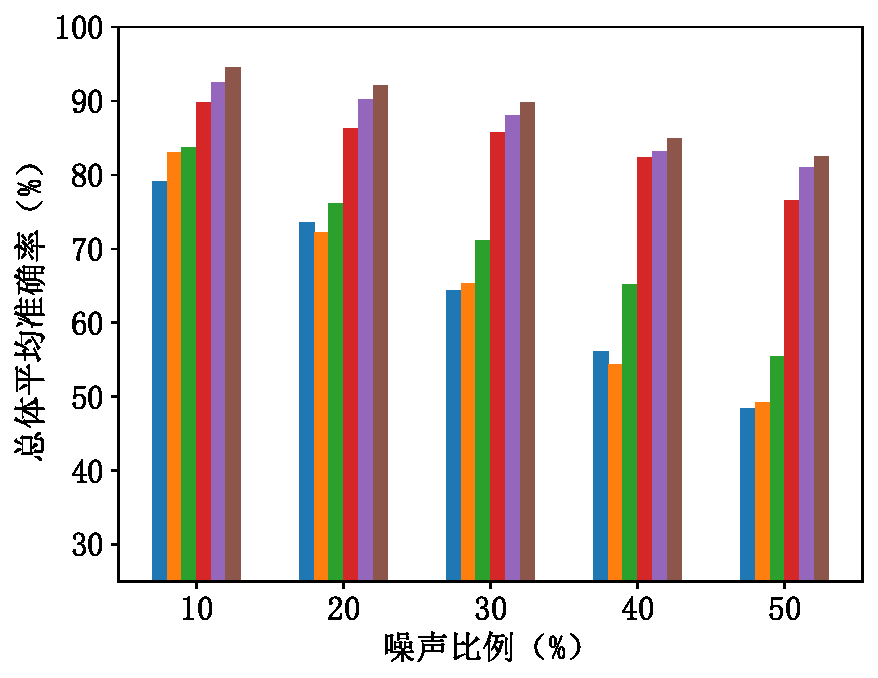
\includegraphics[width=6.24cm]{pic/chapter4/ober/noise_sy.pdf}
  }
  \subfloat[]{
    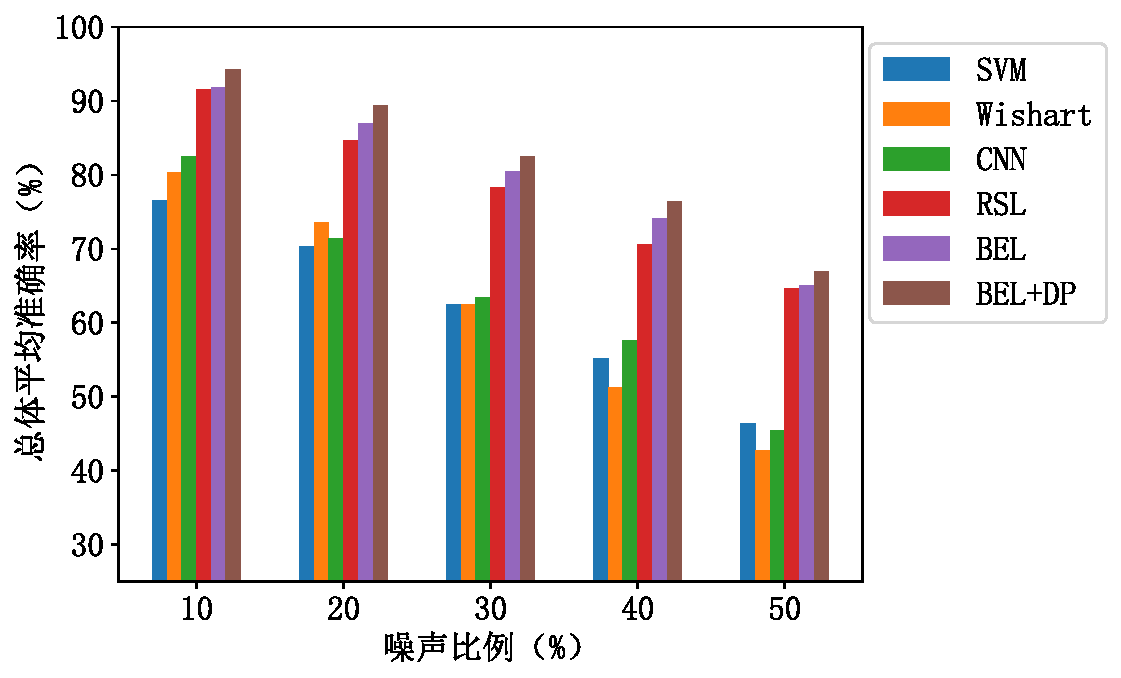
\includegraphics[width=8.04cm]{pic/chapter4/ober/noise_in.pdf}
  }
  \caption{ESAR Oberpfaffenhofen地区数据不同噪声比例下分类准确率结果。(a) 对称噪声源 (b) 非对称噪声源}
  \label{fig:ober_noise}
\end{figure}

\subsection{本章小结}
针对极化SAR图像中存在标签噪声污染问题,本章研究了基于混合模型和边界增强的鲁棒性极化SAR目标分类方法。首先介绍了有限混合模型,并分析了两种混合模型的优缺点。在此基础上,通过深度学习在包含标签噪声样本下训练损失分布存在差异,提出了基于混合模型的样本概率估计方法。同时,为了增强模型对边界信息的感知能力,充分利用边界样本信息,对极化SAR的Pauli伪彩图使用Sobel算子提取边界并膨胀,对膨胀边界内样本进行损失增强。最后,提出了动态的自学习损失函数,通过噪声样本概率动态调整模型预测与真值标签的依赖,实现模型的鲁棒性训练过程。最终,本章通过在两个真实极化SARS数据集,对两种噪声源进行模拟实验,验证本章方法的有效性与优越性。同时,还对不同噪声比例下各个方法的分类准确率进行了比较,进一步验证本章方法的有效性与优越性。